\addtocontents{toc}{\protect\clearpage\protect\noindent Table of Contents
(Continued)}
\addtocontents{toc}{\protect\medskip}
\addtocontents{toc}{\protect\flushright Page}

\chapter{Empirical Results}\label{empiric}

This chapter describes the results of a financial markets analysis of the {\em Challenger} accident. The first section describes the five companies studied. They are Morton Thiokol, the manufacturer of the solid rocket boosters that failed; Rockwell International and its subsidiary Rocketdyne, the manufacturer of the main orbiter and the shuttle's main engines, respectively; Martin Marietta, the manufacturer of the external tank; Lockheed, the firm that prepared the shuttle between missions; and Grumman, the firm that operated the ground control computers.

The next section discusses what we would hypothesize to happen after the explosion of the {\em Challenger}. That is, the null hypothesis that we wish to disprove is that due to the accident we would expect the shuttle operations to shut down, generating no revenue for the shuttle contractors.

The next section discusses what we actually found. The shuttle firms did experience losses, but Morton Thiokol experienced an approximately twelve percent decline value, and nearly four percent of the company's shares traded that day. Morton Thiokol experienced substantial negative returns.

\section{Company Data}

Five shuttle contractors are analyzed for the market's reaction to the shuttle accident. The firms are Morton Thiokol, Rockwell International, Lockheed, Grumman, and Martin Marietta. Lockheed controls the largest portion of the shuttle contract, some seventy five percent \cite{wsjfirms}. The next largest holders of shuttle business are Grumman and Morton Thiokol. Table~\ref{financial} contains financial data for the companies under study.

\begin{table}[h!]
\caption{Financial data for firms studied.}
\sffamily
\begin{tabular*}{6in}{l@{\extracolsep{.3ex}}rrrrr}
\hline\hline       
 & Morton & Rockwell & Martin &          &         \\
 & Thiokol & International & Marietta & Lockheed & Grumman \\
\hline
Shares Outstanding & & & & & \\
(millions, 1986) & 47.08 & 287.78 &  56.31 &  65.61 &  32.60 \\
 & & & & & \\
Sales & & & & & \\
(millions \$, 1985) & 1,832.30 & 11,338.00 & 4,410.10 & 9,535.00 & 3,048.50 \\
 & & & & & \\
Earnings Per & & & & & \\
Share (1985) & 2.44 &   1.96 &   3.05 &   6.10 &   2.65 \\
 & & & & & \\
Profit margin & & & & & \\
(1985) & 6.5 & 5.3 &   4.0 &   4.2 &   2.7  \\
 & & & & & \\
Long-term debt & & & & & \\
(millions \$, 1985) & 152.7 & 647.5 & 220.4 &  35.0 & 263.4 \\
 & & & & & \\
Market value & & & & & \\
(Jan. 27, 1986, & & & & & \\
millions \$) & 1,736.075 & 10,144.245 & 1,949.734 & 3,067.270 & 884.275 \\ \hline
\end{tabular*}
\label{financial}
\end{table}

From the table it can be seen that Morton is the smallest in terms of sales, but when viewed from a market-value perspective, they are twice Grumman's size and almost the same size as Martin Marietta. Lockheed has the least long term debt, followed by Morton Thiokol.

\subsection{Rockwell International}

Rockwell International built the space shuttle {\em Challenger}. Its subsidiary, Rocketdyne, built the shuttle's main engines. Rockwell provided spare parts and consulting on the shuttle, as they had built all that NASA was using at the time.

\subsection{Morton Thiokol}

Morton Thiokol was a well diversified company at the time of the accident. According to Value Line, thirty four percent of sales are specialty chemicals, forty seven percent are aerospace (this includes solid rocket motors, flares, and munitions), nineteen percent salt (Morton salt) \cite{vlmti486}. Value Line predicted in April, 1986, that Morton Thiokol would suffer five to ten cent decline per quarter in earnings \cite{vlmti486}. Value Line also states: ``As to any liability for the [shuttle] accident, indemnifications and insurance appear to provide full protection'' \cite{vlmti486}. Further, Value Line, states, ``the reduced [launch] schedule makes competition from a second booster rocket source unlikely, as does the required high cost and long development time'' \cite{vlmti486}. Thus, according to analysts at Value Line, Morton Thiokol would be expected to face lower returns only because of a loss of sales due to the accident.

\subsection{Lockheed}

Lockheed held the contract to prepare the space shuttle for launch. Lockheed controlled some seventy five percent of the shuttle contract \cite{wsjfirms}. They would thus be expected to be impacted by the shutdown of shuttle operations after the accident. Additionally, according to Value Line, Lockheed would also face a loss of revenue in satellite construction due to the space shuttle standstill \cite{vllock786}.

\subsection{Grumman}

Grumman operated the ground control computers at the time of the accident. They were after Lockheed in terms of revenue from the shuttle program. As with Lockheed, we would expect the firm to experience negative returns the day of the accident.

\subsection{Martin Marietta}

Martin Marietta manufactured the external tank. The external tank was implicated by the {\em New York Times} the day after the accident \cite{nytexternal}. The external tank was a continuing source of revenue for Martin Marietta.

\section{Results}

The null hypothesis that we used is that due to the accident, all of the firms under study should experience negative returns due to a loss of revenue from the space shuttle program standstill. The market would, according to the efficient markets theory, incorporate this new information into the prices of the firms in question. Analyzing the returns for the five firms under study shows that they all (except Grumman) received negative returns on the day of the accident. This is shown in Table~\ref{returns}. The day of the accident is marked.

%\begin{table}[htbp]

\begin{table}[h!]
\caption{Returns for market and five firms studied.}
\sffamily
\begin{tabular*}{6in}{r@{\extracolsep{.5ex}}rrrrrr}
\hline\hline       
       & Market & Morton & Rockwell & Martin &          &         \\
Date$\;$  & ({\footnotesize EWRETD}) & Thiokol & International & Marietta & Lockheed & Grumman \\
\hline
860124 &   0.008 &   0.010 &   0.000 &   0.038 &   0.019 &   0.009 \\
860127 &   0.002 &   0.010 &   0.000 &   0.011 &   0.003 &  -0.048 \\
$\bullet$860128 &   0.003 &  -0.119 &  -0.025 &  -0.032 &  -0.021 &   0.005 \\
860129 &  -0.006 &  -0.015 &   0.018 &  -0.011 &   0.011 &   0.009 \\
860130 &   0.003 &   0.008 &  -0.011 &   0.000 &   0.000 &  -0.014 \\
860131 &   0.007 &  -0.031 &   0.022 &   0.004 &  -0.003 &   0.014 \\
860203 &   0.005 &   0.032 &   0.028 &   0.023 &   0.005 &   0.023 \\
860204 &  -0.005 &   0.023 &   0.017 &   0.022 &   0.022 &   0.000 \\ \hline
\end{tabular*}
\label{returns}
\end{table}

Morton Thiokol was a different case. On the day of the accident, Morton Thiokol experienced a negative twelve percent return. This allows us to reject the null hypothesis that Morton Thiokol would experience a loss because of the shuttle program shutdown. Rather, it indicates that the market guessed that Morton Thiokol would experience more future losses than the other firms.

Shares traded data for Morton Thiokol is also skewed. The volume of shares that traded hands increased nearly ten times over the previous day, as shown in Table~\ref{volume}. The day of the accident is marked.

\begin{table}[h!]
\caption{Shares traded (volume) for firms studied.}
\sffamily
\begin{tabular*}{6in}{r@{\extracolsep{1em}}rrrrr}
\hline\hline       
       &  Morton & Rockwell & Martin &          &         \\
Date   &  Thiokol & International & Marietta & Lockheed & Grumman \\
\hline
860124 & 85,100 & 136,900 & 182,600 & 181,700 & 26,200 \\
860127 & 190,300 & 73,000 & 117,500 & 226,600 & 98,700 \\
$\bullet$860128 & 1,739,900 & 563,200 & 446,200 & 667,500 & 34,500 \\
860129 & 1,680,500 & 252,500 & 840,300 & 364,900 & 31,300 \\
860130 & 730,100 & 154,000 & 212,800 & 329,600 & 146,300 \\
860131 & 895,400 & 179,900 & 163,000 & 603,400 & 90,400 \\
860203 & 1,516,900 & 204,600 & 287,700 & 479,600 & 43,200 \\
860204 & 972,200 & 400,500 & 605,200 & 739,100 & 31,900 \\ \hline
\end{tabular*}
\label{volume}
\end{table}

Most firms experienced increases in volume on the day of the accident (except Grumman). Morton Thiokol's volume increased so nearly four percent of its total shares outstanding traded (although some shares traded more than once). Martin Marietta experienced a 1.5 percent turnover in shares outstanding, double the volume of the previous day. Recall that it appeared on the day of the accident that the external tank, manufactured by Martin Marietta, had caused the accident. Table~\ref{percenttraded} shows the percentage turnover of each firms stocks. The table was created using 1986 data on shares outstanding. The day of the accident is marked.

\begin{table}[h!]
\caption{Percent shares traded (volume/shars outstanding
$\times$ 100) for firms studied.}
\sffamily
\begin{tabular*}{6in}{r@{\extracolsep{1em}}rrrrr}
\hline\hline       
       &  Morton & Rockwell & Martin &          &         \\
Date   &  Thiokol & International & Marietta & Lockheed & Grumman \\
\hline
860124 &   0.18 &   0.05 &   0.32 &   0.28 &   0.08  \\
860127 &   0.40 &   0.03 &   0.21 &   0.35 &   0.30  \\
$\bullet$860128 &   3.70 &   0.20 &   0.79 &   1.02 &   0.11  \\
860129 &   3.57 &   0.09 &   1.49 &   0.56 &   0.10  \\
860130 &   1.55 &   0.05 &   0.38 &   0.50 &   0.45  \\
860131 &   1.90 &   0.06 &   0.29 &   0.92 &   0.28  \\
860203 &   3.22 &   0.07 &   0.51 &   0.73 &   0.13  \\
860204 &   2.07 &   0.14 &   1.07 &   1.13 &   0.10  \\ \hline
\end{tabular*}
\label{percenttraded}
\end{table}

Figure~\ref{thvol} shows graphically the increase in volume
for Morton Thiokol.

\begin{figure}[hp]
\begin{center}
%% GNUPLOT: LaTeX picture
\setlength{\unitlength}{0.240900pt}
\ifx\plotpoint\undefined\newsavebox{\plotpoint}\fi
\sbox{\plotpoint}{\rule[-0.175pt]{0.350pt}{0.350pt}}%
\begin{picture}(1500,900)(0,0)
%\tenrm
\put(264,158){\rule[-0.175pt]{282.335pt}{0.350pt}}
\put(264,158){\rule[-0.175pt]{282.335pt}{0.350pt}}
\put(264,158){\rule[-0.175pt]{4.818pt}{0.350pt}}
\put(242,158){\makebox(0,0)[r]{0}}
\put(1416,158){\rule[-0.175pt]{4.818pt}{0.350pt}}
\put(264,228){\rule[-0.175pt]{282.335pt}{0.350pt}}
\put(264,228){\rule[-0.175pt]{4.818pt}{0.350pt}}
\put(242,228){\makebox(0,0)[r]{200,000}}
\put(1416,228){\rule[-0.175pt]{4.818pt}{0.350pt}}
\put(264,298){\rule[-0.175pt]{282.335pt}{0.350pt}}
\put(264,298){\rule[-0.175pt]{4.818pt}{0.350pt}}
\put(242,298){\makebox(0,0)[r]{400,000}}
\put(1416,298){\rule[-0.175pt]{4.818pt}{0.350pt}}
\put(264,368){\rule[-0.175pt]{282.335pt}{0.350pt}}
\put(264,368){\rule[-0.175pt]{4.818pt}{0.350pt}}
\put(242,368){\makebox(0,0)[r]{600,000}}
\put(1416,368){\rule[-0.175pt]{4.818pt}{0.350pt}}
\put(264,438){\rule[-0.175pt]{282.335pt}{0.350pt}}
\put(264,438){\rule[-0.175pt]{4.818pt}{0.350pt}}
\put(242,438){\makebox(0,0)[r]{800,000}}
\put(1416,438){\rule[-0.175pt]{4.818pt}{0.350pt}}
\put(264,507){\rule[-0.175pt]{282.335pt}{0.350pt}}
\put(264,507){\rule[-0.175pt]{4.818pt}{0.350pt}}
\put(242,507){\makebox(0,0)[r]{1,000,000}}
\put(1416,507){\rule[-0.175pt]{4.818pt}{0.350pt}}
\put(264,577){\rule[-0.175pt]{282.335pt}{0.350pt}}
\put(264,577){\rule[-0.175pt]{4.818pt}{0.350pt}}
\put(242,577){\makebox(0,0)[r]{1,200,000}}
\put(1416,577){\rule[-0.175pt]{4.818pt}{0.350pt}}
\put(264,647){\rule[-0.175pt]{282.335pt}{0.350pt}}
\put(264,647){\rule[-0.175pt]{4.818pt}{0.350pt}}
\put(242,647){\makebox(0,0)[r]{1,400,000}}
\put(1416,647){\rule[-0.175pt]{4.818pt}{0.350pt}}
\put(264,717){\rule[-0.175pt]{282.335pt}{0.350pt}}
\put(264,717){\rule[-0.175pt]{4.818pt}{0.350pt}}
\put(242,717){\makebox(0,0)[r]{1,600,000}}
\put(1416,717){\rule[-0.175pt]{4.818pt}{0.350pt}}
\put(264,787){\rule[-0.175pt]{282.335pt}{0.350pt}}
\put(264,787){\rule[-0.175pt]{4.818pt}{0.350pt}}
\put(242,787){\makebox(0,0)[r]{1,800,000}}
\put(1416,787){\rule[-0.175pt]{4.818pt}{0.350pt}}
\put(695,158){\rule[-0.175pt]{0.350pt}{151.526pt}}
\put(695,158){\rule[-0.175pt]{0.350pt}{4.818pt}}
\put(695,113){\makebox(0,0){Challenger}}
\put(695,767){\rule[-0.175pt]{0.350pt}{4.818pt}}
\put(264,158){\rule[-0.175pt]{282.335pt}{0.350pt}}
\put(1436,158){\rule[-0.175pt]{0.350pt}{151.526pt}}
\put(264,787){\rule[-0.175pt]{282.335pt}{0.350pt}}
\put(850,832){\makebox(0,0){Morton Thiokol Volume}}
\put(264,158){\rule[-0.175pt]{0.350pt}{151.526pt}}
\put(264,175){\usebox{\plotpoint}}
\put(264,175){\usebox{\plotpoint}}
\put(265,176){\usebox{\plotpoint}}
\put(266,177){\usebox{\plotpoint}}
\put(267,178){\usebox{\plotpoint}}
\put(268,179){\usebox{\plotpoint}}
\put(269,180){\usebox{\plotpoint}}
\put(270,181){\usebox{\plotpoint}}
\put(271,182){\usebox{\plotpoint}}
\put(272,184){\usebox{\plotpoint}}
\put(273,185){\usebox{\plotpoint}}
\put(274,186){\usebox{\plotpoint}}
\put(275,187){\usebox{\plotpoint}}
\put(276,188){\usebox{\plotpoint}}
\put(277,189){\usebox{\plotpoint}}
\put(278,190){\usebox{\plotpoint}}
\put(279,191){\usebox{\plotpoint}}
\put(280,193){\usebox{\plotpoint}}
\put(281,194){\usebox{\plotpoint}}
\put(282,195){\usebox{\plotpoint}}
\put(283,196){\usebox{\plotpoint}}
\put(284,197){\usebox{\plotpoint}}
\put(285,198){\usebox{\plotpoint}}
\put(286,199){\usebox{\plotpoint}}
\put(287,200){\usebox{\plotpoint}}
\put(288,200){\usebox{\plotpoint}}
\put(289,199){\usebox{\plotpoint}}
\put(290,198){\usebox{\plotpoint}}
\put(291,197){\usebox{\plotpoint}}
\put(292,195){\usebox{\plotpoint}}
\put(293,194){\usebox{\plotpoint}}
\put(294,193){\usebox{\plotpoint}}
\put(295,192){\usebox{\plotpoint}}
\put(296,191){\usebox{\plotpoint}}
\put(297,189){\usebox{\plotpoint}}
\put(298,188){\usebox{\plotpoint}}
\put(299,187){\usebox{\plotpoint}}
\put(300,186){\usebox{\plotpoint}}
\put(301,185){\usebox{\plotpoint}}
\put(302,183){\usebox{\plotpoint}}
\put(303,182){\usebox{\plotpoint}}
\put(304,181){\usebox{\plotpoint}}
\put(305,180){\usebox{\plotpoint}}
\put(306,179){\usebox{\plotpoint}}
\put(307,177){\usebox{\plotpoint}}
\put(308,176){\usebox{\plotpoint}}
\put(309,175){\usebox{\plotpoint}}
\put(310,174){\usebox{\plotpoint}}
\put(311,173){\usebox{\plotpoint}}
\put(312,173){\usebox{\plotpoint}}
\put(312,173){\rule[-0.175pt]{0.350pt}{0.743pt}}
\put(313,176){\rule[-0.175pt]{0.350pt}{0.743pt}}
\put(314,179){\rule[-0.175pt]{0.350pt}{0.743pt}}
\put(315,182){\rule[-0.175pt]{0.350pt}{0.743pt}}
\put(316,185){\rule[-0.175pt]{0.350pt}{0.743pt}}
\put(317,188){\rule[-0.175pt]{0.350pt}{0.743pt}}
\put(318,191){\rule[-0.175pt]{0.350pt}{0.743pt}}
\put(319,194){\rule[-0.175pt]{0.350pt}{0.743pt}}
\put(320,197){\rule[-0.175pt]{0.350pt}{0.743pt}}
\put(321,200){\rule[-0.175pt]{0.350pt}{0.743pt}}
\put(322,203){\rule[-0.175pt]{0.350pt}{0.743pt}}
\put(323,206){\rule[-0.175pt]{0.350pt}{0.743pt}}
\put(324,209){\rule[-0.175pt]{0.350pt}{0.743pt}}
\put(325,213){\rule[-0.175pt]{0.350pt}{0.743pt}}
\put(326,216){\rule[-0.175pt]{0.350pt}{0.743pt}}
\put(327,219){\rule[-0.175pt]{0.350pt}{0.743pt}}
\put(328,222){\rule[-0.175pt]{0.350pt}{0.743pt}}
\put(329,225){\rule[-0.175pt]{0.350pt}{0.743pt}}
\put(330,228){\rule[-0.175pt]{0.350pt}{0.743pt}}
\put(331,231){\rule[-0.175pt]{0.350pt}{0.743pt}}
\put(332,234){\rule[-0.175pt]{0.350pt}{0.743pt}}
\put(333,237){\rule[-0.175pt]{0.350pt}{0.743pt}}
\put(334,240){\rule[-0.175pt]{0.350pt}{0.743pt}}
\put(335,243){\rule[-0.175pt]{0.350pt}{0.743pt}}
\put(336,246){\usebox{\plotpoint}}
\put(336,244){\rule[-0.175pt]{0.350pt}{0.562pt}}
\put(337,242){\rule[-0.175pt]{0.350pt}{0.562pt}}
\put(338,240){\rule[-0.175pt]{0.350pt}{0.562pt}}
\put(339,237){\rule[-0.175pt]{0.350pt}{0.562pt}}
\put(340,235){\rule[-0.175pt]{0.350pt}{0.562pt}}
\put(341,233){\rule[-0.175pt]{0.350pt}{0.562pt}}
\put(342,230){\rule[-0.175pt]{0.350pt}{0.562pt}}
\put(343,228){\rule[-0.175pt]{0.350pt}{0.562pt}}
\put(344,226){\rule[-0.175pt]{0.350pt}{0.562pt}}
\put(345,223){\rule[-0.175pt]{0.350pt}{0.562pt}}
\put(346,221){\rule[-0.175pt]{0.350pt}{0.562pt}}
\put(347,219){\rule[-0.175pt]{0.350pt}{0.562pt}}
\put(348,216){\rule[-0.175pt]{0.350pt}{0.562pt}}
\put(349,214){\rule[-0.175pt]{0.350pt}{0.562pt}}
\put(350,212){\rule[-0.175pt]{0.350pt}{0.562pt}}
\put(351,209){\rule[-0.175pt]{0.350pt}{0.562pt}}
\put(352,207){\rule[-0.175pt]{0.350pt}{0.562pt}}
\put(353,205){\rule[-0.175pt]{0.350pt}{0.562pt}}
\put(354,202){\rule[-0.175pt]{0.350pt}{0.562pt}}
\put(355,200){\rule[-0.175pt]{0.350pt}{0.562pt}}
\put(356,198){\rule[-0.175pt]{0.350pt}{0.562pt}}
\put(357,195){\rule[-0.175pt]{0.350pt}{0.562pt}}
\put(358,193){\rule[-0.175pt]{0.350pt}{0.562pt}}
\put(359,191){\rule[-0.175pt]{0.350pt}{0.562pt}}
\put(360,191){\usebox{\plotpoint}}
\put(360,191){\rule[-0.175pt]{1.156pt}{0.350pt}}
\put(364,192){\rule[-0.175pt]{1.156pt}{0.350pt}}
\put(369,193){\rule[-0.175pt]{1.156pt}{0.350pt}}
\put(374,194){\rule[-0.175pt]{1.156pt}{0.350pt}}
\put(379,195){\rule[-0.175pt]{1.156pt}{0.350pt}}
\put(383,196){\rule[-0.175pt]{0.385pt}{0.350pt}}
\put(385,197){\rule[-0.175pt]{0.385pt}{0.350pt}}
\put(387,198){\rule[-0.175pt]{0.385pt}{0.350pt}}
\put(388,199){\rule[-0.175pt]{0.385pt}{0.350pt}}
\put(390,200){\rule[-0.175pt]{0.385pt}{0.350pt}}
\put(392,201){\rule[-0.175pt]{0.385pt}{0.350pt}}
\put(393,202){\rule[-0.175pt]{0.385pt}{0.350pt}}
\put(395,203){\rule[-0.175pt]{0.385pt}{0.350pt}}
\put(396,204){\rule[-0.175pt]{0.385pt}{0.350pt}}
\put(398,205){\rule[-0.175pt]{0.385pt}{0.350pt}}
\put(400,206){\rule[-0.175pt]{0.385pt}{0.350pt}}
\put(401,207){\rule[-0.175pt]{0.385pt}{0.350pt}}
\put(403,208){\rule[-0.175pt]{0.385pt}{0.350pt}}
\put(404,209){\rule[-0.175pt]{0.385pt}{0.350pt}}
\put(406,210){\rule[-0.175pt]{0.385pt}{0.350pt}}
\put(408,209){\usebox{\plotpoint}}
\put(409,208){\usebox{\plotpoint}}
\put(410,207){\usebox{\plotpoint}}
\put(411,205){\usebox{\plotpoint}}
\put(412,204){\usebox{\plotpoint}}
\put(413,203){\usebox{\plotpoint}}
\put(414,201){\usebox{\plotpoint}}
\put(415,200){\usebox{\plotpoint}}
\put(416,199){\usebox{\plotpoint}}
\put(417,197){\usebox{\plotpoint}}
\put(418,196){\usebox{\plotpoint}}
\put(419,195){\usebox{\plotpoint}}
\put(420,194){\usebox{\plotpoint}}
\put(421,192){\usebox{\plotpoint}}
\put(422,191){\usebox{\plotpoint}}
\put(423,190){\usebox{\plotpoint}}
\put(424,188){\usebox{\plotpoint}}
\put(425,187){\usebox{\plotpoint}}
\put(426,186){\usebox{\plotpoint}}
\put(427,184){\usebox{\plotpoint}}
\put(428,183){\usebox{\plotpoint}}
\put(429,182){\usebox{\plotpoint}}
\put(430,181){\usebox{\plotpoint}}
\put(431,181){\rule[-0.175pt]{0.350pt}{0.361pt}}
\put(432,182){\rule[-0.175pt]{0.350pt}{0.361pt}}
\put(433,184){\rule[-0.175pt]{0.350pt}{0.361pt}}
\put(434,185){\rule[-0.175pt]{0.350pt}{0.361pt}}
\put(435,187){\rule[-0.175pt]{0.350pt}{0.361pt}}
\put(436,188){\rule[-0.175pt]{0.350pt}{0.361pt}}
\put(437,190){\rule[-0.175pt]{0.350pt}{0.361pt}}
\put(438,191){\rule[-0.175pt]{0.350pt}{0.361pt}}
\put(439,193){\rule[-0.175pt]{0.350pt}{0.361pt}}
\put(440,194){\rule[-0.175pt]{0.350pt}{0.361pt}}
\put(441,196){\rule[-0.175pt]{0.350pt}{0.361pt}}
\put(442,197){\rule[-0.175pt]{0.350pt}{0.361pt}}
\put(443,199){\rule[-0.175pt]{0.350pt}{0.361pt}}
\put(444,200){\rule[-0.175pt]{0.350pt}{0.361pt}}
\put(445,202){\rule[-0.175pt]{0.350pt}{0.361pt}}
\put(446,203){\rule[-0.175pt]{0.350pt}{0.361pt}}
\put(447,205){\rule[-0.175pt]{0.350pt}{0.361pt}}
\put(448,206){\rule[-0.175pt]{0.350pt}{0.361pt}}
\put(449,208){\rule[-0.175pt]{0.350pt}{0.361pt}}
\put(450,209){\rule[-0.175pt]{0.350pt}{0.361pt}}
\put(451,211){\rule[-0.175pt]{0.350pt}{0.361pt}}
\put(452,212){\rule[-0.175pt]{0.350pt}{0.361pt}}
\put(453,214){\rule[-0.175pt]{0.350pt}{0.361pt}}
\put(454,215){\rule[-0.175pt]{0.350pt}{0.361pt}}
\put(455,215){\rule[-0.175pt]{0.350pt}{0.361pt}}
\put(456,214){\rule[-0.175pt]{0.350pt}{0.361pt}}
\put(457,212){\rule[-0.175pt]{0.350pt}{0.361pt}}
\put(458,211){\rule[-0.175pt]{0.350pt}{0.361pt}}
\put(459,209){\rule[-0.175pt]{0.350pt}{0.361pt}}
\put(460,208){\rule[-0.175pt]{0.350pt}{0.361pt}}
\put(461,206){\rule[-0.175pt]{0.350pt}{0.361pt}}
\put(462,205){\rule[-0.175pt]{0.350pt}{0.361pt}}
\put(463,203){\rule[-0.175pt]{0.350pt}{0.361pt}}
\put(464,202){\rule[-0.175pt]{0.350pt}{0.361pt}}
\put(465,200){\rule[-0.175pt]{0.350pt}{0.361pt}}
\put(466,199){\rule[-0.175pt]{0.350pt}{0.361pt}}
\put(467,197){\rule[-0.175pt]{0.350pt}{0.361pt}}
\put(468,196){\rule[-0.175pt]{0.350pt}{0.361pt}}
\put(469,194){\rule[-0.175pt]{0.350pt}{0.361pt}}
\put(470,193){\rule[-0.175pt]{0.350pt}{0.361pt}}
\put(471,191){\rule[-0.175pt]{0.350pt}{0.361pt}}
\put(472,190){\rule[-0.175pt]{0.350pt}{0.361pt}}
\put(473,188){\rule[-0.175pt]{0.350pt}{0.361pt}}
\put(474,187){\rule[-0.175pt]{0.350pt}{0.361pt}}
\put(475,185){\rule[-0.175pt]{0.350pt}{0.361pt}}
\put(476,184){\rule[-0.175pt]{0.350pt}{0.361pt}}
\put(477,182){\rule[-0.175pt]{0.350pt}{0.361pt}}
\put(478,181){\rule[-0.175pt]{0.350pt}{0.361pt}}
\put(479,181){\usebox{\plotpoint}}
\put(480,182){\usebox{\plotpoint}}
\put(481,183){\usebox{\plotpoint}}
\put(482,184){\usebox{\plotpoint}}
\put(483,185){\usebox{\plotpoint}}
\put(484,186){\usebox{\plotpoint}}
\put(485,187){\usebox{\plotpoint}}
\put(486,188){\usebox{\plotpoint}}
\put(487,189){\usebox{\plotpoint}}
\put(488,190){\usebox{\plotpoint}}
\put(489,191){\usebox{\plotpoint}}
\put(490,192){\usebox{\plotpoint}}
\put(491,193){\usebox{\plotpoint}}
\put(492,195){\usebox{\plotpoint}}
\put(493,196){\usebox{\plotpoint}}
\put(494,197){\usebox{\plotpoint}}
\put(495,198){\usebox{\plotpoint}}
\put(496,199){\usebox{\plotpoint}}
\put(497,200){\usebox{\plotpoint}}
\put(498,201){\usebox{\plotpoint}}
\put(499,202){\usebox{\plotpoint}}
\put(500,203){\usebox{\plotpoint}}
\put(501,204){\usebox{\plotpoint}}
\put(502,205){\usebox{\plotpoint}}
\put(503,206){\usebox{\plotpoint}}
\put(503,207){\usebox{\plotpoint}}
\put(504,208){\usebox{\plotpoint}}
\put(505,209){\usebox{\plotpoint}}
\put(507,210){\usebox{\plotpoint}}
\put(508,211){\usebox{\plotpoint}}
\put(510,212){\usebox{\plotpoint}}
\put(511,213){\usebox{\plotpoint}}
\put(512,214){\usebox{\plotpoint}}
\put(514,215){\usebox{\plotpoint}}
\put(515,216){\usebox{\plotpoint}}
\put(517,217){\usebox{\plotpoint}}
\put(518,218){\usebox{\plotpoint}}
\put(519,219){\usebox{\plotpoint}}
\put(521,220){\usebox{\plotpoint}}
\put(522,221){\usebox{\plotpoint}}
\put(524,222){\usebox{\plotpoint}}
\put(525,223){\usebox{\plotpoint}}
\put(526,224){\usebox{\plotpoint}}
\put(527,221){\rule[-0.175pt]{0.350pt}{0.532pt}}
\put(528,219){\rule[-0.175pt]{0.350pt}{0.532pt}}
\put(529,217){\rule[-0.175pt]{0.350pt}{0.532pt}}
\put(530,215){\rule[-0.175pt]{0.350pt}{0.532pt}}
\put(531,212){\rule[-0.175pt]{0.350pt}{0.532pt}}
\put(532,210){\rule[-0.175pt]{0.350pt}{0.532pt}}
\put(533,208){\rule[-0.175pt]{0.350pt}{0.532pt}}
\put(534,206){\rule[-0.175pt]{0.350pt}{0.532pt}}
\put(535,204){\rule[-0.175pt]{0.350pt}{0.532pt}}
\put(536,201){\rule[-0.175pt]{0.350pt}{0.532pt}}
\put(537,199){\rule[-0.175pt]{0.350pt}{0.532pt}}
\put(538,197){\rule[-0.175pt]{0.350pt}{0.532pt}}
\put(539,195){\rule[-0.175pt]{0.350pt}{0.532pt}}
\put(540,193){\rule[-0.175pt]{0.350pt}{0.532pt}}
\put(541,190){\rule[-0.175pt]{0.350pt}{0.532pt}}
\put(542,188){\rule[-0.175pt]{0.350pt}{0.532pt}}
\put(543,186){\rule[-0.175pt]{0.350pt}{0.532pt}}
\put(544,184){\rule[-0.175pt]{0.350pt}{0.532pt}}
\put(545,182){\rule[-0.175pt]{0.350pt}{0.532pt}}
\put(546,179){\rule[-0.175pt]{0.350pt}{0.532pt}}
\put(547,177){\rule[-0.175pt]{0.350pt}{0.532pt}}
\put(548,175){\rule[-0.175pt]{0.350pt}{0.532pt}}
\put(549,173){\rule[-0.175pt]{0.350pt}{0.532pt}}
\put(550,171){\rule[-0.175pt]{0.350pt}{0.532pt}}
\put(551,171){\usebox{\plotpoint}}
\put(551,171){\usebox{\plotpoint}}
\put(552,172){\usebox{\plotpoint}}
\put(553,173){\usebox{\plotpoint}}
\put(554,174){\usebox{\plotpoint}}
\put(555,175){\usebox{\plotpoint}}
\put(557,176){\usebox{\plotpoint}}
\put(558,177){\usebox{\plotpoint}}
\put(559,178){\usebox{\plotpoint}}
\put(560,179){\usebox{\plotpoint}}
\put(561,180){\usebox{\plotpoint}}
\put(563,181){\usebox{\plotpoint}}
\put(564,182){\usebox{\plotpoint}}
\put(565,183){\usebox{\plotpoint}}
\put(566,184){\usebox{\plotpoint}}
\put(567,185){\usebox{\plotpoint}}
\put(569,186){\usebox{\plotpoint}}
\put(570,187){\usebox{\plotpoint}}
\put(571,188){\usebox{\plotpoint}}
\put(572,189){\usebox{\plotpoint}}
\put(573,190){\usebox{\plotpoint}}
\put(575,191){\rule[-0.175pt]{0.482pt}{0.350pt}}
\put(577,190){\rule[-0.175pt]{0.482pt}{0.350pt}}
\put(579,189){\rule[-0.175pt]{0.482pt}{0.350pt}}
\put(581,188){\rule[-0.175pt]{0.482pt}{0.350pt}}
\put(583,187){\rule[-0.175pt]{0.482pt}{0.350pt}}
\put(585,186){\rule[-0.175pt]{0.482pt}{0.350pt}}
\put(587,185){\rule[-0.175pt]{0.482pt}{0.350pt}}
\put(589,184){\rule[-0.175pt]{0.482pt}{0.350pt}}
\put(591,183){\rule[-0.175pt]{0.482pt}{0.350pt}}
\put(593,182){\rule[-0.175pt]{0.482pt}{0.350pt}}
\put(595,181){\rule[-0.175pt]{0.482pt}{0.350pt}}
\put(597,180){\rule[-0.175pt]{0.482pt}{0.350pt}}
\put(599,179){\rule[-0.175pt]{0.385pt}{0.350pt}}
\put(600,180){\rule[-0.175pt]{0.385pt}{0.350pt}}
\put(602,181){\rule[-0.175pt]{0.385pt}{0.350pt}}
\put(603,182){\rule[-0.175pt]{0.385pt}{0.350pt}}
\put(605,183){\rule[-0.175pt]{0.385pt}{0.350pt}}
\put(606,184){\rule[-0.175pt]{0.385pt}{0.350pt}}
\put(608,185){\rule[-0.175pt]{0.385pt}{0.350pt}}
\put(610,186){\rule[-0.175pt]{0.385pt}{0.350pt}}
\put(611,187){\rule[-0.175pt]{0.385pt}{0.350pt}}
\put(613,188){\rule[-0.175pt]{0.385pt}{0.350pt}}
\put(614,189){\rule[-0.175pt]{0.385pt}{0.350pt}}
\put(616,190){\rule[-0.175pt]{0.385pt}{0.350pt}}
\put(618,191){\rule[-0.175pt]{0.385pt}{0.350pt}}
\put(619,192){\rule[-0.175pt]{0.385pt}{0.350pt}}
\put(621,193){\rule[-0.175pt]{0.385pt}{0.350pt}}
\put(622,194){\rule[-0.175pt]{0.964pt}{0.350pt}}
\put(627,193){\rule[-0.175pt]{0.964pt}{0.350pt}}
\put(631,192){\rule[-0.175pt]{0.964pt}{0.350pt}}
\put(635,191){\rule[-0.175pt]{0.964pt}{0.350pt}}
\put(639,190){\rule[-0.175pt]{0.964pt}{0.350pt}}
\put(643,189){\rule[-0.175pt]{0.964pt}{0.350pt}}
\put(647,188){\rule[-0.175pt]{0.350pt}{0.361pt}}
\put(648,189){\rule[-0.175pt]{0.350pt}{0.361pt}}
\put(649,191){\rule[-0.175pt]{0.350pt}{0.361pt}}
\put(650,192){\rule[-0.175pt]{0.350pt}{0.361pt}}
\put(651,194){\rule[-0.175pt]{0.350pt}{0.361pt}}
\put(652,195){\rule[-0.175pt]{0.350pt}{0.361pt}}
\put(653,197){\rule[-0.175pt]{0.350pt}{0.361pt}}
\put(654,198){\rule[-0.175pt]{0.350pt}{0.361pt}}
\put(655,200){\rule[-0.175pt]{0.350pt}{0.361pt}}
\put(656,201){\rule[-0.175pt]{0.350pt}{0.361pt}}
\put(657,203){\rule[-0.175pt]{0.350pt}{0.361pt}}
\put(658,204){\rule[-0.175pt]{0.350pt}{0.361pt}}
\put(659,206){\rule[-0.175pt]{0.350pt}{0.361pt}}
\put(660,207){\rule[-0.175pt]{0.350pt}{0.361pt}}
\put(661,209){\rule[-0.175pt]{0.350pt}{0.361pt}}
\put(662,210){\rule[-0.175pt]{0.350pt}{0.361pt}}
\put(663,212){\rule[-0.175pt]{0.350pt}{0.361pt}}
\put(664,213){\rule[-0.175pt]{0.350pt}{0.361pt}}
\put(665,215){\rule[-0.175pt]{0.350pt}{0.361pt}}
\put(666,216){\rule[-0.175pt]{0.350pt}{0.361pt}}
\put(667,218){\rule[-0.175pt]{0.350pt}{0.361pt}}
\put(668,219){\rule[-0.175pt]{0.350pt}{0.361pt}}
\put(669,221){\rule[-0.175pt]{0.350pt}{0.361pt}}
\put(670,222){\rule[-0.175pt]{0.350pt}{0.361pt}}
\put(671,224){\rule[-0.175pt]{0.350pt}{5.440pt}}
\put(672,246){\rule[-0.175pt]{0.350pt}{5.440pt}}
\put(673,269){\rule[-0.175pt]{0.350pt}{5.440pt}}
\put(674,291){\rule[-0.175pt]{0.350pt}{5.440pt}}
\put(675,314){\rule[-0.175pt]{0.350pt}{5.440pt}}
\put(676,336){\rule[-0.175pt]{0.350pt}{5.440pt}}
\put(677,359){\rule[-0.175pt]{0.350pt}{5.440pt}}
\put(678,382){\rule[-0.175pt]{0.350pt}{5.440pt}}
\put(679,404){\rule[-0.175pt]{0.350pt}{5.440pt}}
\put(680,427){\rule[-0.175pt]{0.350pt}{5.440pt}}
\put(681,449){\rule[-0.175pt]{0.350pt}{5.440pt}}
\put(682,472){\rule[-0.175pt]{0.350pt}{5.440pt}}
\put(683,495){\rule[-0.175pt]{0.350pt}{5.440pt}}
\put(684,517){\rule[-0.175pt]{0.350pt}{5.440pt}}
\put(685,540){\rule[-0.175pt]{0.350pt}{5.440pt}}
\put(686,562){\rule[-0.175pt]{0.350pt}{5.440pt}}
\put(687,585){\rule[-0.175pt]{0.350pt}{5.440pt}}
\put(688,607){\rule[-0.175pt]{0.350pt}{5.440pt}}
\put(689,630){\rule[-0.175pt]{0.350pt}{5.440pt}}
\put(690,653){\rule[-0.175pt]{0.350pt}{5.440pt}}
\put(691,675){\rule[-0.175pt]{0.350pt}{5.440pt}}
\put(692,698){\rule[-0.175pt]{0.350pt}{5.440pt}}
\put(693,720){\rule[-0.175pt]{0.350pt}{5.440pt}}
\put(694,743){\rule[-0.175pt]{0.350pt}{5.440pt}}
\put(695,765){\usebox{\plotpoint}}
\put(695,766){\usebox{\plotpoint}}
\put(696,765){\usebox{\plotpoint}}
\put(697,764){\usebox{\plotpoint}}
\put(698,763){\usebox{\plotpoint}}
\put(699,762){\usebox{\plotpoint}}
\put(700,761){\usebox{\plotpoint}}
\put(701,760){\usebox{\plotpoint}}
\put(702,759){\usebox{\plotpoint}}
\put(703,758){\usebox{\plotpoint}}
\put(704,757){\usebox{\plotpoint}}
\put(705,756){\usebox{\plotpoint}}
\put(707,755){\usebox{\plotpoint}}
\put(708,754){\usebox{\plotpoint}}
\put(709,753){\usebox{\plotpoint}}
\put(710,752){\usebox{\plotpoint}}
\put(711,751){\usebox{\plotpoint}}
\put(712,750){\usebox{\plotpoint}}
\put(713,749){\usebox{\plotpoint}}
\put(714,748){\usebox{\plotpoint}}
\put(715,747){\usebox{\plotpoint}}
\put(716,746){\usebox{\plotpoint}}
\put(717,745){\usebox{\plotpoint}}
\put(718,731){\rule[-0.175pt]{0.350pt}{3.332pt}}
\put(719,717){\rule[-0.175pt]{0.350pt}{3.332pt}}
\put(720,703){\rule[-0.175pt]{0.350pt}{3.332pt}}
\put(721,689){\rule[-0.175pt]{0.350pt}{3.332pt}}
\put(722,675){\rule[-0.175pt]{0.350pt}{3.332pt}}
\put(723,662){\rule[-0.175pt]{0.350pt}{3.332pt}}
\put(724,648){\rule[-0.175pt]{0.350pt}{3.332pt}}
\put(725,634){\rule[-0.175pt]{0.350pt}{3.332pt}}
\put(726,620){\rule[-0.175pt]{0.350pt}{3.332pt}}
\put(727,606){\rule[-0.175pt]{0.350pt}{3.332pt}}
\put(728,592){\rule[-0.175pt]{0.350pt}{3.332pt}}
\put(729,579){\rule[-0.175pt]{0.350pt}{3.332pt}}
\put(730,565){\rule[-0.175pt]{0.350pt}{3.332pt}}
\put(731,551){\rule[-0.175pt]{0.350pt}{3.332pt}}
\put(732,537){\rule[-0.175pt]{0.350pt}{3.332pt}}
\put(733,523){\rule[-0.175pt]{0.350pt}{3.332pt}}
\put(734,509){\rule[-0.175pt]{0.350pt}{3.332pt}}
\put(735,496){\rule[-0.175pt]{0.350pt}{3.332pt}}
\put(736,482){\rule[-0.175pt]{0.350pt}{3.332pt}}
\put(737,468){\rule[-0.175pt]{0.350pt}{3.332pt}}
\put(738,454){\rule[-0.175pt]{0.350pt}{3.332pt}}
\put(739,440){\rule[-0.175pt]{0.350pt}{3.332pt}}
\put(740,426){\rule[-0.175pt]{0.350pt}{3.332pt}}
\put(741,413){\rule[-0.175pt]{0.350pt}{3.332pt}}
\put(742,413){\usebox{\plotpoint}}
\put(742,413){\rule[-0.175pt]{0.350pt}{0.582pt}}
\put(743,415){\rule[-0.175pt]{0.350pt}{0.582pt}}
\put(744,417){\rule[-0.175pt]{0.350pt}{0.582pt}}
\put(745,420){\rule[-0.175pt]{0.350pt}{0.582pt}}
\put(746,422){\rule[-0.175pt]{0.350pt}{0.582pt}}
\put(747,425){\rule[-0.175pt]{0.350pt}{0.582pt}}
\put(748,427){\rule[-0.175pt]{0.350pt}{0.582pt}}
\put(749,429){\rule[-0.175pt]{0.350pt}{0.582pt}}
\put(750,432){\rule[-0.175pt]{0.350pt}{0.582pt}}
\put(751,434){\rule[-0.175pt]{0.350pt}{0.582pt}}
\put(752,437){\rule[-0.175pt]{0.350pt}{0.582pt}}
\put(753,439){\rule[-0.175pt]{0.350pt}{0.582pt}}
\put(754,441){\rule[-0.175pt]{0.350pt}{0.582pt}}
\put(755,444){\rule[-0.175pt]{0.350pt}{0.582pt}}
\put(756,446){\rule[-0.175pt]{0.350pt}{0.582pt}}
\put(757,449){\rule[-0.175pt]{0.350pt}{0.582pt}}
\put(758,451){\rule[-0.175pt]{0.350pt}{0.582pt}}
\put(759,454){\rule[-0.175pt]{0.350pt}{0.582pt}}
\put(760,456){\rule[-0.175pt]{0.350pt}{0.582pt}}
\put(761,458){\rule[-0.175pt]{0.350pt}{0.582pt}}
\put(762,461){\rule[-0.175pt]{0.350pt}{0.582pt}}
\put(763,463){\rule[-0.175pt]{0.350pt}{0.582pt}}
\put(764,466){\rule[-0.175pt]{0.350pt}{0.582pt}}
\put(765,468){\rule[-0.175pt]{0.350pt}{0.582pt}}
\put(766,470){\rule[-0.175pt]{0.350pt}{2.178pt}}
\put(767,480){\rule[-0.175pt]{0.350pt}{2.178pt}}
\put(768,489){\rule[-0.175pt]{0.350pt}{2.178pt}}
\put(769,498){\rule[-0.175pt]{0.350pt}{2.178pt}}
\put(770,507){\rule[-0.175pt]{0.350pt}{2.178pt}}
\put(771,516){\rule[-0.175pt]{0.350pt}{2.178pt}}
\put(772,525){\rule[-0.175pt]{0.350pt}{2.178pt}}
\put(773,534){\rule[-0.175pt]{0.350pt}{2.178pt}}
\put(774,543){\rule[-0.175pt]{0.350pt}{2.178pt}}
\put(775,552){\rule[-0.175pt]{0.350pt}{2.178pt}}
\put(776,561){\rule[-0.175pt]{0.350pt}{2.178pt}}
\put(777,570){\rule[-0.175pt]{0.350pt}{2.178pt}}
\put(778,579){\rule[-0.175pt]{0.350pt}{2.178pt}}
\put(779,588){\rule[-0.175pt]{0.350pt}{2.178pt}}
\put(780,597){\rule[-0.175pt]{0.350pt}{2.178pt}}
\put(781,606){\rule[-0.175pt]{0.350pt}{2.178pt}}
\put(782,615){\rule[-0.175pt]{0.350pt}{2.178pt}}
\put(783,624){\rule[-0.175pt]{0.350pt}{2.178pt}}
\put(784,633){\rule[-0.175pt]{0.350pt}{2.178pt}}
\put(785,642){\rule[-0.175pt]{0.350pt}{2.178pt}}
\put(786,651){\rule[-0.175pt]{0.350pt}{2.178pt}}
\put(787,660){\rule[-0.175pt]{0.350pt}{2.178pt}}
\put(788,669){\rule[-0.175pt]{0.350pt}{2.178pt}}
\put(789,678){\rule[-0.175pt]{0.350pt}{2.178pt}}
\put(790,680){\rule[-0.175pt]{0.350pt}{1.907pt}}
\put(791,672){\rule[-0.175pt]{0.350pt}{1.907pt}}
\put(792,664){\rule[-0.175pt]{0.350pt}{1.907pt}}
\put(793,656){\rule[-0.175pt]{0.350pt}{1.907pt}}
\put(794,648){\rule[-0.175pt]{0.350pt}{1.907pt}}
\put(795,640){\rule[-0.175pt]{0.350pt}{1.907pt}}
\put(796,632){\rule[-0.175pt]{0.350pt}{1.907pt}}
\put(797,624){\rule[-0.175pt]{0.350pt}{1.907pt}}
\put(798,616){\rule[-0.175pt]{0.350pt}{1.907pt}}
\put(799,608){\rule[-0.175pt]{0.350pt}{1.907pt}}
\put(800,600){\rule[-0.175pt]{0.350pt}{1.907pt}}
\put(801,592){\rule[-0.175pt]{0.350pt}{1.907pt}}
\put(802,585){\rule[-0.175pt]{0.350pt}{1.907pt}}
\put(803,577){\rule[-0.175pt]{0.350pt}{1.907pt}}
\put(804,569){\rule[-0.175pt]{0.350pt}{1.907pt}}
\put(805,561){\rule[-0.175pt]{0.350pt}{1.907pt}}
\put(806,553){\rule[-0.175pt]{0.350pt}{1.907pt}}
\put(807,545){\rule[-0.175pt]{0.350pt}{1.907pt}}
\put(808,537){\rule[-0.175pt]{0.350pt}{1.907pt}}
\put(809,529){\rule[-0.175pt]{0.350pt}{1.907pt}}
\put(810,521){\rule[-0.175pt]{0.350pt}{1.907pt}}
\put(811,513){\rule[-0.175pt]{0.350pt}{1.907pt}}
\put(812,505){\rule[-0.175pt]{0.350pt}{1.907pt}}
\put(813,498){\rule[-0.175pt]{0.350pt}{1.907pt}}
\put(814,496){\usebox{\plotpoint}}
\put(815,495){\usebox{\plotpoint}}
\put(816,493){\usebox{\plotpoint}}
\put(817,492){\usebox{\plotpoint}}
\put(818,491){\usebox{\plotpoint}}
\put(819,489){\usebox{\plotpoint}}
\put(820,488){\usebox{\plotpoint}}
\put(821,487){\usebox{\plotpoint}}
\put(822,485){\usebox{\plotpoint}}
\put(823,484){\usebox{\plotpoint}}
\put(824,482){\usebox{\plotpoint}}
\put(825,481){\usebox{\plotpoint}}
\put(826,480){\usebox{\plotpoint}}
\put(827,478){\usebox{\plotpoint}}
\put(828,477){\usebox{\plotpoint}}
\put(829,476){\usebox{\plotpoint}}
\put(830,474){\usebox{\plotpoint}}
\put(831,473){\usebox{\plotpoint}}
\put(832,471){\usebox{\plotpoint}}
\put(833,470){\usebox{\plotpoint}}
\put(834,469){\usebox{\plotpoint}}
\put(835,467){\usebox{\plotpoint}}
\put(836,466){\usebox{\plotpoint}}
\put(837,465){\usebox{\plotpoint}}
\put(838,458){\rule[-0.175pt]{0.350pt}{1.556pt}}
\put(839,452){\rule[-0.175pt]{0.350pt}{1.556pt}}
\put(840,445){\rule[-0.175pt]{0.350pt}{1.556pt}}
\put(841,439){\rule[-0.175pt]{0.350pt}{1.556pt}}
\put(842,432){\rule[-0.175pt]{0.350pt}{1.556pt}}
\put(843,426){\rule[-0.175pt]{0.350pt}{1.556pt}}
\put(844,419){\rule[-0.175pt]{0.350pt}{1.556pt}}
\put(845,413){\rule[-0.175pt]{0.350pt}{1.556pt}}
\put(846,406){\rule[-0.175pt]{0.350pt}{1.556pt}}
\put(847,400){\rule[-0.175pt]{0.350pt}{1.556pt}}
\put(848,393){\rule[-0.175pt]{0.350pt}{1.556pt}}
\put(849,387){\rule[-0.175pt]{0.350pt}{1.556pt}}
\put(850,381){\rule[-0.175pt]{0.350pt}{1.556pt}}
\put(851,374){\rule[-0.175pt]{0.350pt}{1.556pt}}
\put(852,368){\rule[-0.175pt]{0.350pt}{1.556pt}}
\put(853,361){\rule[-0.175pt]{0.350pt}{1.556pt}}
\put(854,355){\rule[-0.175pt]{0.350pt}{1.556pt}}
\put(855,348){\rule[-0.175pt]{0.350pt}{1.556pt}}
\put(856,342){\rule[-0.175pt]{0.350pt}{1.556pt}}
\put(857,335){\rule[-0.175pt]{0.350pt}{1.556pt}}
\put(858,329){\rule[-0.175pt]{0.350pt}{1.556pt}}
\put(859,322){\rule[-0.175pt]{0.350pt}{1.556pt}}
\put(860,316){\rule[-0.175pt]{0.350pt}{1.556pt}}
\put(861,310){\rule[-0.175pt]{0.350pt}{1.556pt}}
\put(862,310){\rule[-0.175pt]{0.350pt}{0.391pt}}
\put(863,311){\rule[-0.175pt]{0.350pt}{0.391pt}}
\put(864,313){\rule[-0.175pt]{0.350pt}{0.391pt}}
\put(865,314){\rule[-0.175pt]{0.350pt}{0.391pt}}
\put(866,316){\rule[-0.175pt]{0.350pt}{0.391pt}}
\put(867,318){\rule[-0.175pt]{0.350pt}{0.391pt}}
\put(868,319){\rule[-0.175pt]{0.350pt}{0.391pt}}
\put(869,321){\rule[-0.175pt]{0.350pt}{0.391pt}}
\put(870,323){\rule[-0.175pt]{0.350pt}{0.391pt}}
\put(871,324){\rule[-0.175pt]{0.350pt}{0.391pt}}
\put(872,326){\rule[-0.175pt]{0.350pt}{0.391pt}}
\put(873,327){\rule[-0.175pt]{0.350pt}{0.391pt}}
\put(874,329){\rule[-0.175pt]{0.350pt}{0.391pt}}
\put(875,331){\rule[-0.175pt]{0.350pt}{0.391pt}}
\put(876,332){\rule[-0.175pt]{0.350pt}{0.391pt}}
\put(877,334){\rule[-0.175pt]{0.350pt}{0.391pt}}
\put(878,336){\rule[-0.175pt]{0.350pt}{0.391pt}}
\put(879,337){\rule[-0.175pt]{0.350pt}{0.391pt}}
\put(880,339){\rule[-0.175pt]{0.350pt}{0.391pt}}
\put(881,340){\rule[-0.175pt]{0.350pt}{0.391pt}}
\put(882,342){\rule[-0.175pt]{0.350pt}{0.391pt}}
\put(883,344){\rule[-0.175pt]{0.350pt}{0.391pt}}
\put(884,345){\rule[-0.175pt]{0.350pt}{0.391pt}}
\put(885,347){\rule[-0.175pt]{0.350pt}{0.391pt}}
\put(886,346){\rule[-0.175pt]{0.350pt}{0.572pt}}
\put(887,344){\rule[-0.175pt]{0.350pt}{0.572pt}}
\put(888,341){\rule[-0.175pt]{0.350pt}{0.572pt}}
\put(889,339){\rule[-0.175pt]{0.350pt}{0.572pt}}
\put(890,337){\rule[-0.175pt]{0.350pt}{0.572pt}}
\put(891,334){\rule[-0.175pt]{0.350pt}{0.572pt}}
\put(892,332){\rule[-0.175pt]{0.350pt}{0.572pt}}
\put(893,330){\rule[-0.175pt]{0.350pt}{0.572pt}}
\put(894,327){\rule[-0.175pt]{0.350pt}{0.572pt}}
\put(895,325){\rule[-0.175pt]{0.350pt}{0.572pt}}
\put(896,322){\rule[-0.175pt]{0.350pt}{0.572pt}}
\put(897,320){\rule[-0.175pt]{0.350pt}{0.572pt}}
\put(898,318){\rule[-0.175pt]{0.350pt}{0.572pt}}
\put(899,315){\rule[-0.175pt]{0.350pt}{0.572pt}}
\put(900,313){\rule[-0.175pt]{0.350pt}{0.572pt}}
\put(901,311){\rule[-0.175pt]{0.350pt}{0.572pt}}
\put(902,308){\rule[-0.175pt]{0.350pt}{0.572pt}}
\put(903,306){\rule[-0.175pt]{0.350pt}{0.572pt}}
\put(904,303){\rule[-0.175pt]{0.350pt}{0.572pt}}
\put(905,301){\rule[-0.175pt]{0.350pt}{0.572pt}}
\put(906,299){\rule[-0.175pt]{0.350pt}{0.572pt}}
\put(907,296){\rule[-0.175pt]{0.350pt}{0.572pt}}
\put(908,294){\rule[-0.175pt]{0.350pt}{0.572pt}}
\put(909,292){\rule[-0.175pt]{0.350pt}{0.572pt}}
\put(910,290){\rule[-0.175pt]{0.350pt}{0.462pt}}
\put(911,288){\rule[-0.175pt]{0.350pt}{0.462pt}}
\put(912,286){\rule[-0.175pt]{0.350pt}{0.462pt}}
\put(913,284){\rule[-0.175pt]{0.350pt}{0.462pt}}
\put(914,282){\rule[-0.175pt]{0.350pt}{0.462pt}}
\put(915,280){\rule[-0.175pt]{0.350pt}{0.462pt}}
\put(916,278){\rule[-0.175pt]{0.350pt}{0.462pt}}
\put(917,276){\rule[-0.175pt]{0.350pt}{0.462pt}}
\put(918,274){\rule[-0.175pt]{0.350pt}{0.462pt}}
\put(919,272){\rule[-0.175pt]{0.350pt}{0.462pt}}
\put(920,270){\rule[-0.175pt]{0.350pt}{0.462pt}}
\put(921,269){\rule[-0.175pt]{0.350pt}{0.462pt}}
\put(922,267){\rule[-0.175pt]{0.350pt}{0.462pt}}
\put(923,265){\rule[-0.175pt]{0.350pt}{0.462pt}}
\put(924,263){\rule[-0.175pt]{0.350pt}{0.462pt}}
\put(925,261){\rule[-0.175pt]{0.350pt}{0.462pt}}
\put(926,259){\rule[-0.175pt]{0.350pt}{0.462pt}}
\put(927,257){\rule[-0.175pt]{0.350pt}{0.462pt}}
\put(928,255){\rule[-0.175pt]{0.350pt}{0.462pt}}
\put(929,253){\rule[-0.175pt]{0.350pt}{0.462pt}}
\put(930,251){\rule[-0.175pt]{0.350pt}{0.462pt}}
\put(931,249){\rule[-0.175pt]{0.350pt}{0.462pt}}
\put(932,247){\rule[-0.175pt]{0.350pt}{0.462pt}}
\put(933,246){\rule[-0.175pt]{0.350pt}{0.462pt}}
\put(934,246){\usebox{\plotpoint}}
\put(934,246){\rule[-0.175pt]{2.891pt}{0.350pt}}
\put(946,247){\rule[-0.175pt]{2.891pt}{0.350pt}}
\put(958,248){\rule[-0.175pt]{0.350pt}{0.733pt}}
\put(959,251){\rule[-0.175pt]{0.350pt}{0.733pt}}
\put(960,254){\rule[-0.175pt]{0.350pt}{0.733pt}}
\put(961,257){\rule[-0.175pt]{0.350pt}{0.733pt}}
\put(962,260){\rule[-0.175pt]{0.350pt}{0.733pt}}
\put(963,263){\rule[-0.175pt]{0.350pt}{0.733pt}}
\put(964,266){\rule[-0.175pt]{0.350pt}{0.733pt}}
\put(965,269){\rule[-0.175pt]{0.350pt}{0.733pt}}
\put(966,272){\rule[-0.175pt]{0.350pt}{0.733pt}}
\put(967,275){\rule[-0.175pt]{0.350pt}{0.733pt}}
\put(968,278){\rule[-0.175pt]{0.350pt}{0.733pt}}
\put(969,281){\rule[-0.175pt]{0.350pt}{0.733pt}}
\put(970,284){\rule[-0.175pt]{0.350pt}{0.733pt}}
\put(971,287){\rule[-0.175pt]{0.350pt}{0.733pt}}
\put(972,290){\rule[-0.175pt]{0.350pt}{0.733pt}}
\put(973,293){\rule[-0.175pt]{0.350pt}{0.733pt}}
\put(974,296){\rule[-0.175pt]{0.350pt}{0.733pt}}
\put(975,299){\rule[-0.175pt]{0.350pt}{0.733pt}}
\put(976,302){\rule[-0.175pt]{0.350pt}{0.733pt}}
\put(977,305){\rule[-0.175pt]{0.350pt}{0.733pt}}
\put(978,308){\rule[-0.175pt]{0.350pt}{0.733pt}}
\put(979,311){\rule[-0.175pt]{0.350pt}{0.733pt}}
\put(980,314){\rule[-0.175pt]{0.350pt}{0.733pt}}
\put(981,317){\rule[-0.175pt]{0.350pt}{0.733pt}}
\put(982,320){\usebox{\plotpoint}}
\put(982,317){\rule[-0.175pt]{0.350pt}{0.848pt}}
\put(983,313){\rule[-0.175pt]{0.350pt}{0.848pt}}
\put(984,310){\rule[-0.175pt]{0.350pt}{0.848pt}}
\put(985,306){\rule[-0.175pt]{0.350pt}{0.848pt}}
\put(986,303){\rule[-0.175pt]{0.350pt}{0.848pt}}
\put(987,299){\rule[-0.175pt]{0.350pt}{0.848pt}}
\put(988,296){\rule[-0.175pt]{0.350pt}{0.848pt}}
\put(989,292){\rule[-0.175pt]{0.350pt}{0.848pt}}
\put(990,289){\rule[-0.175pt]{0.350pt}{0.848pt}}
\put(991,285){\rule[-0.175pt]{0.350pt}{0.848pt}}
\put(992,282){\rule[-0.175pt]{0.350pt}{0.848pt}}
\put(993,278){\rule[-0.175pt]{0.350pt}{0.848pt}}
\put(994,275){\rule[-0.175pt]{0.350pt}{0.848pt}}
\put(995,271){\rule[-0.175pt]{0.350pt}{0.848pt}}
\put(996,268){\rule[-0.175pt]{0.350pt}{0.848pt}}
\put(997,264){\rule[-0.175pt]{0.350pt}{0.848pt}}
\put(998,261){\rule[-0.175pt]{0.350pt}{0.848pt}}
\put(999,257){\rule[-0.175pt]{0.350pt}{0.848pt}}
\put(1000,254){\rule[-0.175pt]{0.350pt}{0.848pt}}
\put(1001,250){\rule[-0.175pt]{0.350pt}{0.848pt}}
\put(1002,247){\rule[-0.175pt]{0.350pt}{0.848pt}}
\put(1003,243){\rule[-0.175pt]{0.350pt}{0.848pt}}
\put(1004,240){\rule[-0.175pt]{0.350pt}{0.848pt}}
\put(1005,240){\usebox{\plotpoint}}
\put(1005,240){\usebox{\plotpoint}}
\put(1006,241){\usebox{\plotpoint}}
\put(1007,242){\usebox{\plotpoint}}
\put(1008,243){\usebox{\plotpoint}}
\put(1009,244){\usebox{\plotpoint}}
\put(1010,245){\usebox{\plotpoint}}
\put(1011,246){\usebox{\plotpoint}}
\put(1012,247){\usebox{\plotpoint}}
\put(1013,248){\usebox{\plotpoint}}
\put(1014,249){\usebox{\plotpoint}}
\put(1015,250){\usebox{\plotpoint}}
\put(1016,251){\usebox{\plotpoint}}
\put(1017,252){\usebox{\plotpoint}}
\put(1018,253){\usebox{\plotpoint}}
\put(1019,254){\usebox{\plotpoint}}
\put(1020,255){\usebox{\plotpoint}}
\put(1021,256){\usebox{\plotpoint}}
\put(1022,257){\usebox{\plotpoint}}
\put(1023,258){\usebox{\plotpoint}}
\put(1024,259){\usebox{\plotpoint}}
\put(1025,260){\usebox{\plotpoint}}
\put(1026,261){\usebox{\plotpoint}}
\put(1027,262){\usebox{\plotpoint}}
\put(1028,263){\usebox{\plotpoint}}
\put(1029,263){\rule[-0.175pt]{0.350pt}{0.622pt}}
\put(1030,265){\rule[-0.175pt]{0.350pt}{0.622pt}}
\put(1031,268){\rule[-0.175pt]{0.350pt}{0.622pt}}
\put(1032,270){\rule[-0.175pt]{0.350pt}{0.622pt}}
\put(1033,273){\rule[-0.175pt]{0.350pt}{0.622pt}}
\put(1034,275){\rule[-0.175pt]{0.350pt}{0.622pt}}
\put(1035,278){\rule[-0.175pt]{0.350pt}{0.622pt}}
\put(1036,281){\rule[-0.175pt]{0.350pt}{0.622pt}}
\put(1037,283){\rule[-0.175pt]{0.350pt}{0.622pt}}
\put(1038,286){\rule[-0.175pt]{0.350pt}{0.622pt}}
\put(1039,288){\rule[-0.175pt]{0.350pt}{0.622pt}}
\put(1040,291){\rule[-0.175pt]{0.350pt}{0.622pt}}
\put(1041,294){\rule[-0.175pt]{0.350pt}{0.622pt}}
\put(1042,296){\rule[-0.175pt]{0.350pt}{0.622pt}}
\put(1043,299){\rule[-0.175pt]{0.350pt}{0.622pt}}
\put(1044,301){\rule[-0.175pt]{0.350pt}{0.622pt}}
\put(1045,304){\rule[-0.175pt]{0.350pt}{0.622pt}}
\put(1046,306){\rule[-0.175pt]{0.350pt}{0.622pt}}
\put(1047,309){\rule[-0.175pt]{0.350pt}{0.622pt}}
\put(1048,312){\rule[-0.175pt]{0.350pt}{0.622pt}}
\put(1049,314){\rule[-0.175pt]{0.350pt}{0.622pt}}
\put(1050,317){\rule[-0.175pt]{0.350pt}{0.622pt}}
\put(1051,319){\rule[-0.175pt]{0.350pt}{0.622pt}}
\put(1052,322){\rule[-0.175pt]{0.350pt}{0.622pt}}
\put(1053,325){\usebox{\plotpoint}}
\put(1054,326){\usebox{\plotpoint}}
\put(1055,327){\usebox{\plotpoint}}
\put(1056,329){\usebox{\plotpoint}}
\put(1057,330){\usebox{\plotpoint}}
\put(1058,332){\usebox{\plotpoint}}
\put(1059,333){\usebox{\plotpoint}}
\put(1060,334){\usebox{\plotpoint}}
\put(1061,336){\usebox{\plotpoint}}
\put(1062,337){\usebox{\plotpoint}}
\put(1063,339){\usebox{\plotpoint}}
\put(1064,340){\usebox{\plotpoint}}
\put(1065,341){\usebox{\plotpoint}}
\put(1066,343){\usebox{\plotpoint}}
\put(1067,344){\usebox{\plotpoint}}
\put(1068,346){\usebox{\plotpoint}}
\put(1069,347){\usebox{\plotpoint}}
\put(1070,349){\usebox{\plotpoint}}
\put(1071,350){\usebox{\plotpoint}}
\put(1072,351){\usebox{\plotpoint}}
\put(1073,353){\usebox{\plotpoint}}
\put(1074,354){\usebox{\plotpoint}}
\put(1075,356){\usebox{\plotpoint}}
\put(1076,357){\usebox{\plotpoint}}
\put(1077,358){\usebox{\plotpoint}}
\put(1077,356){\rule[-0.175pt]{0.350pt}{0.512pt}}
\put(1078,354){\rule[-0.175pt]{0.350pt}{0.512pt}}
\put(1079,352){\rule[-0.175pt]{0.350pt}{0.512pt}}
\put(1080,350){\rule[-0.175pt]{0.350pt}{0.512pt}}
\put(1081,348){\rule[-0.175pt]{0.350pt}{0.512pt}}
\put(1082,346){\rule[-0.175pt]{0.350pt}{0.512pt}}
\put(1083,344){\rule[-0.175pt]{0.350pt}{0.512pt}}
\put(1084,342){\rule[-0.175pt]{0.350pt}{0.512pt}}
\put(1085,339){\rule[-0.175pt]{0.350pt}{0.512pt}}
\put(1086,337){\rule[-0.175pt]{0.350pt}{0.512pt}}
\put(1087,335){\rule[-0.175pt]{0.350pt}{0.512pt}}
\put(1088,333){\rule[-0.175pt]{0.350pt}{0.512pt}}
\put(1089,331){\rule[-0.175pt]{0.350pt}{0.512pt}}
\put(1090,329){\rule[-0.175pt]{0.350pt}{0.512pt}}
\put(1091,327){\rule[-0.175pt]{0.350pt}{0.512pt}}
\put(1092,325){\rule[-0.175pt]{0.350pt}{0.512pt}}
\put(1093,322){\rule[-0.175pt]{0.350pt}{0.512pt}}
\put(1094,320){\rule[-0.175pt]{0.350pt}{0.512pt}}
\put(1095,318){\rule[-0.175pt]{0.350pt}{0.512pt}}
\put(1096,316){\rule[-0.175pt]{0.350pt}{0.512pt}}
\put(1097,314){\rule[-0.175pt]{0.350pt}{0.512pt}}
\put(1098,312){\rule[-0.175pt]{0.350pt}{0.512pt}}
\put(1099,310){\rule[-0.175pt]{0.350pt}{0.512pt}}
\put(1100,308){\rule[-0.175pt]{0.350pt}{0.512pt}}
\put(1101,308){\rule[-0.175pt]{0.350pt}{1.044pt}}
\put(1102,312){\rule[-0.175pt]{0.350pt}{1.044pt}}
\put(1103,316){\rule[-0.175pt]{0.350pt}{1.044pt}}
\put(1104,321){\rule[-0.175pt]{0.350pt}{1.044pt}}
\put(1105,325){\rule[-0.175pt]{0.350pt}{1.044pt}}
\put(1106,329){\rule[-0.175pt]{0.350pt}{1.044pt}}
\put(1107,334){\rule[-0.175pt]{0.350pt}{1.044pt}}
\put(1108,338){\rule[-0.175pt]{0.350pt}{1.044pt}}
\put(1109,342){\rule[-0.175pt]{0.350pt}{1.044pt}}
\put(1110,347){\rule[-0.175pt]{0.350pt}{1.044pt}}
\put(1111,351){\rule[-0.175pt]{0.350pt}{1.044pt}}
\put(1112,355){\rule[-0.175pt]{0.350pt}{1.044pt}}
\put(1113,360){\rule[-0.175pt]{0.350pt}{1.044pt}}
\put(1114,364){\rule[-0.175pt]{0.350pt}{1.044pt}}
\put(1115,368){\rule[-0.175pt]{0.350pt}{1.044pt}}
\put(1116,373){\rule[-0.175pt]{0.350pt}{1.044pt}}
\put(1117,377){\rule[-0.175pt]{0.350pt}{1.044pt}}
\put(1118,381){\rule[-0.175pt]{0.350pt}{1.044pt}}
\put(1119,386){\rule[-0.175pt]{0.350pt}{1.044pt}}
\put(1120,390){\rule[-0.175pt]{0.350pt}{1.044pt}}
\put(1121,394){\rule[-0.175pt]{0.350pt}{1.044pt}}
\put(1122,399){\rule[-0.175pt]{0.350pt}{1.044pt}}
\put(1123,403){\rule[-0.175pt]{0.350pt}{1.044pt}}
\put(1124,407){\rule[-0.175pt]{0.350pt}{1.044pt}}
\put(1125,409){\rule[-0.175pt]{0.350pt}{0.572pt}}
\put(1126,407){\rule[-0.175pt]{0.350pt}{0.572pt}}
\put(1127,404){\rule[-0.175pt]{0.350pt}{0.572pt}}
\put(1128,402){\rule[-0.175pt]{0.350pt}{0.572pt}}
\put(1129,400){\rule[-0.175pt]{0.350pt}{0.572pt}}
\put(1130,397){\rule[-0.175pt]{0.350pt}{0.572pt}}
\put(1131,395){\rule[-0.175pt]{0.350pt}{0.572pt}}
\put(1132,393){\rule[-0.175pt]{0.350pt}{0.572pt}}
\put(1133,390){\rule[-0.175pt]{0.350pt}{0.572pt}}
\put(1134,388){\rule[-0.175pt]{0.350pt}{0.572pt}}
\put(1135,385){\rule[-0.175pt]{0.350pt}{0.572pt}}
\put(1136,383){\rule[-0.175pt]{0.350pt}{0.572pt}}
\put(1137,381){\rule[-0.175pt]{0.350pt}{0.572pt}}
\put(1138,378){\rule[-0.175pt]{0.350pt}{0.572pt}}
\put(1139,376){\rule[-0.175pt]{0.350pt}{0.572pt}}
\put(1140,374){\rule[-0.175pt]{0.350pt}{0.572pt}}
\put(1141,371){\rule[-0.175pt]{0.350pt}{0.572pt}}
\put(1142,369){\rule[-0.175pt]{0.350pt}{0.572pt}}
\put(1143,366){\rule[-0.175pt]{0.350pt}{0.572pt}}
\put(1144,364){\rule[-0.175pt]{0.350pt}{0.572pt}}
\put(1145,362){\rule[-0.175pt]{0.350pt}{0.572pt}}
\put(1146,359){\rule[-0.175pt]{0.350pt}{0.572pt}}
\put(1147,357){\rule[-0.175pt]{0.350pt}{0.572pt}}
\put(1148,355){\rule[-0.175pt]{0.350pt}{0.572pt}}
\put(1149,353){\rule[-0.175pt]{0.350pt}{0.472pt}}
\put(1150,351){\rule[-0.175pt]{0.350pt}{0.472pt}}
\put(1151,349){\rule[-0.175pt]{0.350pt}{0.472pt}}
\put(1152,347){\rule[-0.175pt]{0.350pt}{0.472pt}}
\put(1153,345){\rule[-0.175pt]{0.350pt}{0.472pt}}
\put(1154,343){\rule[-0.175pt]{0.350pt}{0.472pt}}
\put(1155,341){\rule[-0.175pt]{0.350pt}{0.472pt}}
\put(1156,339){\rule[-0.175pt]{0.350pt}{0.472pt}}
\put(1157,337){\rule[-0.175pt]{0.350pt}{0.472pt}}
\put(1158,335){\rule[-0.175pt]{0.350pt}{0.472pt}}
\put(1159,333){\rule[-0.175pt]{0.350pt}{0.472pt}}
\put(1160,331){\rule[-0.175pt]{0.350pt}{0.472pt}}
\put(1161,329){\rule[-0.175pt]{0.350pt}{0.472pt}}
\put(1162,327){\rule[-0.175pt]{0.350pt}{0.472pt}}
\put(1163,325){\rule[-0.175pt]{0.350pt}{0.472pt}}
\put(1164,323){\rule[-0.175pt]{0.350pt}{0.472pt}}
\put(1165,321){\rule[-0.175pt]{0.350pt}{0.472pt}}
\put(1166,319){\rule[-0.175pt]{0.350pt}{0.472pt}}
\put(1167,317){\rule[-0.175pt]{0.350pt}{0.472pt}}
\put(1168,315){\rule[-0.175pt]{0.350pt}{0.472pt}}
\put(1169,313){\rule[-0.175pt]{0.350pt}{0.472pt}}
\put(1170,311){\rule[-0.175pt]{0.350pt}{0.472pt}}
\put(1171,309){\rule[-0.175pt]{0.350pt}{0.472pt}}
\put(1172,308){\rule[-0.175pt]{0.350pt}{0.472pt}}
\put(1173,305){\rule[-0.175pt]{0.350pt}{0.492pt}}
\put(1174,303){\rule[-0.175pt]{0.350pt}{0.492pt}}
\put(1175,301){\rule[-0.175pt]{0.350pt}{0.492pt}}
\put(1176,299){\rule[-0.175pt]{0.350pt}{0.492pt}}
\put(1177,297){\rule[-0.175pt]{0.350pt}{0.492pt}}
\put(1178,295){\rule[-0.175pt]{0.350pt}{0.492pt}}
\put(1179,293){\rule[-0.175pt]{0.350pt}{0.492pt}}
\put(1180,291){\rule[-0.175pt]{0.350pt}{0.492pt}}
\put(1181,289){\rule[-0.175pt]{0.350pt}{0.492pt}}
\put(1182,287){\rule[-0.175pt]{0.350pt}{0.492pt}}
\put(1183,285){\rule[-0.175pt]{0.350pt}{0.492pt}}
\put(1184,283){\rule[-0.175pt]{0.350pt}{0.492pt}}
\put(1185,281){\rule[-0.175pt]{0.350pt}{0.492pt}}
\put(1186,279){\rule[-0.175pt]{0.350pt}{0.492pt}}
\put(1187,277){\rule[-0.175pt]{0.350pt}{0.492pt}}
\put(1188,275){\rule[-0.175pt]{0.350pt}{0.492pt}}
\put(1189,273){\rule[-0.175pt]{0.350pt}{0.492pt}}
\put(1190,271){\rule[-0.175pt]{0.350pt}{0.492pt}}
\put(1191,269){\rule[-0.175pt]{0.350pt}{0.492pt}}
\put(1192,267){\rule[-0.175pt]{0.350pt}{0.492pt}}
\put(1193,265){\rule[-0.175pt]{0.350pt}{0.492pt}}
\put(1194,263){\rule[-0.175pt]{0.350pt}{0.492pt}}
\put(1195,261){\rule[-0.175pt]{0.350pt}{0.492pt}}
\put(1196,259){\rule[-0.175pt]{0.350pt}{0.492pt}}
\put(1197,259){\usebox{\plotpoint}}
\put(1197,259){\rule[-0.175pt]{0.350pt}{0.492pt}}
\put(1198,261){\rule[-0.175pt]{0.350pt}{0.492pt}}
\put(1199,263){\rule[-0.175pt]{0.350pt}{0.492pt}}
\put(1200,265){\rule[-0.175pt]{0.350pt}{0.492pt}}
\put(1201,267){\rule[-0.175pt]{0.350pt}{0.492pt}}
\put(1202,269){\rule[-0.175pt]{0.350pt}{0.492pt}}
\put(1203,271){\rule[-0.175pt]{0.350pt}{0.492pt}}
\put(1204,273){\rule[-0.175pt]{0.350pt}{0.492pt}}
\put(1205,275){\rule[-0.175pt]{0.350pt}{0.492pt}}
\put(1206,277){\rule[-0.175pt]{0.350pt}{0.492pt}}
\put(1207,279){\rule[-0.175pt]{0.350pt}{0.492pt}}
\put(1208,281){\rule[-0.175pt]{0.350pt}{0.492pt}}
\put(1209,283){\rule[-0.175pt]{0.350pt}{0.492pt}}
\put(1210,285){\rule[-0.175pt]{0.350pt}{0.492pt}}
\put(1211,287){\rule[-0.175pt]{0.350pt}{0.492pt}}
\put(1212,289){\rule[-0.175pt]{0.350pt}{0.492pt}}
\put(1213,291){\rule[-0.175pt]{0.350pt}{0.492pt}}
\put(1214,293){\rule[-0.175pt]{0.350pt}{0.492pt}}
\put(1215,295){\rule[-0.175pt]{0.350pt}{0.492pt}}
\put(1216,297){\rule[-0.175pt]{0.350pt}{0.492pt}}
\put(1217,299){\rule[-0.175pt]{0.350pt}{0.492pt}}
\put(1218,301){\rule[-0.175pt]{0.350pt}{0.492pt}}
\put(1219,303){\rule[-0.175pt]{0.350pt}{0.492pt}}
\put(1220,305){\rule[-0.175pt]{0.350pt}{0.492pt}}
\put(1221,307){\usebox{\plotpoint}}
\put(1221,305){\rule[-0.175pt]{0.350pt}{0.492pt}}
\put(1222,303){\rule[-0.175pt]{0.350pt}{0.492pt}}
\put(1223,301){\rule[-0.175pt]{0.350pt}{0.492pt}}
\put(1224,299){\rule[-0.175pt]{0.350pt}{0.492pt}}
\put(1225,297){\rule[-0.175pt]{0.350pt}{0.492pt}}
\put(1226,295){\rule[-0.175pt]{0.350pt}{0.492pt}}
\put(1227,293){\rule[-0.175pt]{0.350pt}{0.492pt}}
\put(1228,291){\rule[-0.175pt]{0.350pt}{0.492pt}}
\put(1229,289){\rule[-0.175pt]{0.350pt}{0.492pt}}
\put(1230,287){\rule[-0.175pt]{0.350pt}{0.492pt}}
\put(1231,285){\rule[-0.175pt]{0.350pt}{0.492pt}}
\put(1232,283){\rule[-0.175pt]{0.350pt}{0.492pt}}
\put(1233,281){\rule[-0.175pt]{0.350pt}{0.492pt}}
\put(1234,279){\rule[-0.175pt]{0.350pt}{0.492pt}}
\put(1235,277){\rule[-0.175pt]{0.350pt}{0.492pt}}
\put(1236,275){\rule[-0.175pt]{0.350pt}{0.492pt}}
\put(1237,273){\rule[-0.175pt]{0.350pt}{0.492pt}}
\put(1238,271){\rule[-0.175pt]{0.350pt}{0.492pt}}
\put(1239,269){\rule[-0.175pt]{0.350pt}{0.492pt}}
\put(1240,267){\rule[-0.175pt]{0.350pt}{0.492pt}}
\put(1241,265){\rule[-0.175pt]{0.350pt}{0.492pt}}
\put(1242,263){\rule[-0.175pt]{0.350pt}{0.492pt}}
\put(1243,261){\rule[-0.175pt]{0.350pt}{0.492pt}}
\put(1244,259){\rule[-0.175pt]{0.350pt}{0.492pt}}
\put(1245,259){\usebox{\plotpoint}}
\put(1245,259){\rule[-0.175pt]{5.782pt}{0.350pt}}
\put(1269,258){\rule[-0.175pt]{0.350pt}{0.408pt}}
\put(1270,256){\rule[-0.175pt]{0.350pt}{0.408pt}}
\put(1271,254){\rule[-0.175pt]{0.350pt}{0.408pt}}
\put(1272,253){\rule[-0.175pt]{0.350pt}{0.408pt}}
\put(1273,251){\rule[-0.175pt]{0.350pt}{0.408pt}}
\put(1274,249){\rule[-0.175pt]{0.350pt}{0.408pt}}
\put(1275,248){\rule[-0.175pt]{0.350pt}{0.408pt}}
\put(1276,246){\rule[-0.175pt]{0.350pt}{0.408pt}}
\put(1277,244){\rule[-0.175pt]{0.350pt}{0.408pt}}
\put(1278,243){\rule[-0.175pt]{0.350pt}{0.408pt}}
\put(1279,241){\rule[-0.175pt]{0.350pt}{0.408pt}}
\put(1280,239){\rule[-0.175pt]{0.350pt}{0.408pt}}
\put(1281,237){\rule[-0.175pt]{0.350pt}{0.408pt}}
\put(1282,236){\rule[-0.175pt]{0.350pt}{0.408pt}}
\put(1283,234){\rule[-0.175pt]{0.350pt}{0.408pt}}
\put(1284,232){\rule[-0.175pt]{0.350pt}{0.408pt}}
\put(1285,231){\rule[-0.175pt]{0.350pt}{0.408pt}}
\put(1286,229){\rule[-0.175pt]{0.350pt}{0.408pt}}
\put(1287,227){\rule[-0.175pt]{0.350pt}{0.408pt}}
\put(1288,226){\rule[-0.175pt]{0.350pt}{0.408pt}}
\put(1289,224){\rule[-0.175pt]{0.350pt}{0.408pt}}
\put(1290,222){\rule[-0.175pt]{0.350pt}{0.408pt}}
\put(1291,221){\rule[-0.175pt]{0.350pt}{0.408pt}}
\put(1292,221){\usebox{\plotpoint}}
\put(1292,221){\rule[-0.175pt]{1.927pt}{0.350pt}}
\put(1300,220){\rule[-0.175pt]{1.927pt}{0.350pt}}
\put(1308,219){\rule[-0.175pt]{1.927pt}{0.350pt}}
\put(1316,218){\usebox{\plotpoint}}
\put(1317,219){\usebox{\plotpoint}}
\put(1318,220){\usebox{\plotpoint}}
\put(1320,221){\usebox{\plotpoint}}
\put(1321,222){\usebox{\plotpoint}}
\put(1323,223){\usebox{\plotpoint}}
\put(1324,224){\usebox{\plotpoint}}
\put(1325,225){\usebox{\plotpoint}}
\put(1327,226){\usebox{\plotpoint}}
\put(1328,227){\usebox{\plotpoint}}
\put(1330,228){\usebox{\plotpoint}}
\put(1331,229){\usebox{\plotpoint}}
\put(1332,230){\usebox{\plotpoint}}
\put(1334,231){\usebox{\plotpoint}}
\put(1335,232){\usebox{\plotpoint}}
\put(1337,233){\usebox{\plotpoint}}
\put(1338,234){\usebox{\plotpoint}}
\put(1339,235){\rule[-0.175pt]{0.526pt}{0.350pt}}
\put(1342,236){\rule[-0.175pt]{0.526pt}{0.350pt}}
\put(1344,237){\rule[-0.175pt]{0.526pt}{0.350pt}}
\put(1346,238){\rule[-0.175pt]{0.526pt}{0.350pt}}
\put(1348,239){\rule[-0.175pt]{0.526pt}{0.350pt}}
\put(1350,240){\rule[-0.175pt]{0.526pt}{0.350pt}}
\put(1353,241){\rule[-0.175pt]{0.526pt}{0.350pt}}
\put(1355,242){\rule[-0.175pt]{0.526pt}{0.350pt}}
\put(1357,243){\rule[-0.175pt]{0.526pt}{0.350pt}}
\put(1359,244){\rule[-0.175pt]{0.526pt}{0.350pt}}
\put(1361,245){\rule[-0.175pt]{0.526pt}{0.350pt}}
\put(1363,246){\usebox{\plotpoint}}
\put(1364,246){\rule[-0.175pt]{0.350pt}{0.522pt}}
\put(1365,248){\rule[-0.175pt]{0.350pt}{0.522pt}}
\put(1366,250){\rule[-0.175pt]{0.350pt}{0.522pt}}
\put(1367,252){\rule[-0.175pt]{0.350pt}{0.522pt}}
\put(1368,254){\rule[-0.175pt]{0.350pt}{0.522pt}}
\put(1369,256){\rule[-0.175pt]{0.350pt}{0.522pt}}
\put(1370,259){\rule[-0.175pt]{0.350pt}{0.522pt}}
\put(1371,261){\rule[-0.175pt]{0.350pt}{0.522pt}}
\put(1372,263){\rule[-0.175pt]{0.350pt}{0.522pt}}
\put(1373,265){\rule[-0.175pt]{0.350pt}{0.522pt}}
\put(1374,267){\rule[-0.175pt]{0.350pt}{0.522pt}}
\put(1375,269){\rule[-0.175pt]{0.350pt}{0.522pt}}
\put(1376,271){\rule[-0.175pt]{0.350pt}{0.522pt}}
\put(1377,274){\rule[-0.175pt]{0.350pt}{0.522pt}}
\put(1378,276){\rule[-0.175pt]{0.350pt}{0.522pt}}
\put(1379,278){\rule[-0.175pt]{0.350pt}{0.522pt}}
\put(1380,280){\rule[-0.175pt]{0.350pt}{0.522pt}}
\put(1381,282){\rule[-0.175pt]{0.350pt}{0.522pt}}
\put(1382,284){\rule[-0.175pt]{0.350pt}{0.522pt}}
\put(1383,287){\rule[-0.175pt]{0.350pt}{0.522pt}}
\put(1384,289){\rule[-0.175pt]{0.350pt}{0.522pt}}
\put(1385,291){\rule[-0.175pt]{0.350pt}{0.522pt}}
\put(1386,293){\rule[-0.175pt]{0.350pt}{0.522pt}}
\put(1387,295){\rule[-0.175pt]{0.350pt}{0.522pt}}
\put(1388,297){\rule[-0.175pt]{0.350pt}{0.502pt}}
\put(1389,300){\rule[-0.175pt]{0.350pt}{0.502pt}}
\put(1390,302){\rule[-0.175pt]{0.350pt}{0.502pt}}
\put(1391,304){\rule[-0.175pt]{0.350pt}{0.502pt}}
\put(1392,306){\rule[-0.175pt]{0.350pt}{0.502pt}}
\put(1393,308){\rule[-0.175pt]{0.350pt}{0.502pt}}
\put(1394,310){\rule[-0.175pt]{0.350pt}{0.502pt}}
\put(1395,312){\rule[-0.175pt]{0.350pt}{0.502pt}}
\put(1396,314){\rule[-0.175pt]{0.350pt}{0.502pt}}
\put(1397,316){\rule[-0.175pt]{0.350pt}{0.502pt}}
\put(1398,318){\rule[-0.175pt]{0.350pt}{0.502pt}}
\put(1399,320){\rule[-0.175pt]{0.350pt}{0.502pt}}
\put(1400,323){\rule[-0.175pt]{0.350pt}{0.502pt}}
\put(1401,325){\rule[-0.175pt]{0.350pt}{0.502pt}}
\put(1402,327){\rule[-0.175pt]{0.350pt}{0.502pt}}
\put(1403,329){\rule[-0.175pt]{0.350pt}{0.502pt}}
\put(1404,331){\rule[-0.175pt]{0.350pt}{0.502pt}}
\put(1405,333){\rule[-0.175pt]{0.350pt}{0.502pt}}
\put(1406,335){\rule[-0.175pt]{0.350pt}{0.502pt}}
\put(1407,337){\rule[-0.175pt]{0.350pt}{0.502pt}}
\put(1408,339){\rule[-0.175pt]{0.350pt}{0.502pt}}
\put(1409,341){\rule[-0.175pt]{0.350pt}{0.502pt}}
\put(1410,343){\rule[-0.175pt]{0.350pt}{0.502pt}}
\put(1411,345){\rule[-0.175pt]{0.350pt}{0.502pt}}
\put(1412,343){\rule[-0.175pt]{0.350pt}{1.044pt}}
\put(1413,339){\rule[-0.175pt]{0.350pt}{1.044pt}}
\put(1414,334){\rule[-0.175pt]{0.350pt}{1.044pt}}
\put(1415,330){\rule[-0.175pt]{0.350pt}{1.044pt}}
\put(1416,326){\rule[-0.175pt]{0.350pt}{1.044pt}}
\put(1417,321){\rule[-0.175pt]{0.350pt}{1.044pt}}
\put(1418,317){\rule[-0.175pt]{0.350pt}{1.044pt}}
\put(1419,313){\rule[-0.175pt]{0.350pt}{1.044pt}}
\put(1420,308){\rule[-0.175pt]{0.350pt}{1.044pt}}
\put(1421,304){\rule[-0.175pt]{0.350pt}{1.044pt}}
\put(1422,300){\rule[-0.175pt]{0.350pt}{1.044pt}}
\put(1423,295){\rule[-0.175pt]{0.350pt}{1.044pt}}
\put(1424,291){\rule[-0.175pt]{0.350pt}{1.044pt}}
\put(1425,287){\rule[-0.175pt]{0.350pt}{1.044pt}}
\put(1426,282){\rule[-0.175pt]{0.350pt}{1.044pt}}
\put(1427,278){\rule[-0.175pt]{0.350pt}{1.044pt}}
\put(1428,274){\rule[-0.175pt]{0.350pt}{1.044pt}}
\put(1429,269){\rule[-0.175pt]{0.350pt}{1.044pt}}
\put(1430,265){\rule[-0.175pt]{0.350pt}{1.044pt}}
\put(1431,261){\rule[-0.175pt]{0.350pt}{1.044pt}}
\put(1432,256){\rule[-0.175pt]{0.350pt}{1.044pt}}
\put(1433,252){\rule[-0.175pt]{0.350pt}{1.044pt}}
\put(1434,248){\rule[-0.175pt]{0.350pt}{1.044pt}}
\put(1435,244){\rule[-0.175pt]{0.350pt}{1.044pt}}
\end{picture}

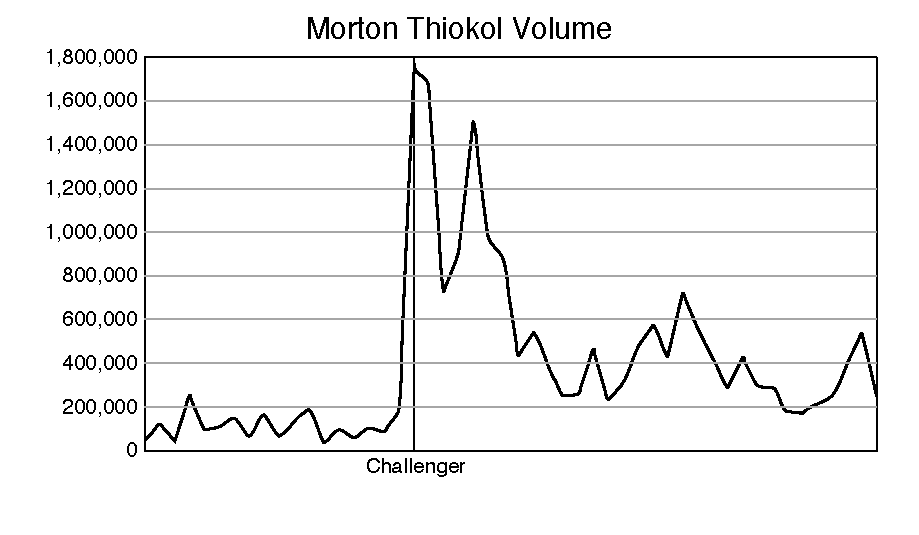
\includegraphics{thvol-final}
\end{center}
\caption{Morton Thiokol volume for 50 days from January 2,
1986 to March 13, 1986.}
\label{thvol}
\end{figure}


Another indication of the market's belief that Morton Thiokol would experience larger than normal losses (than the other shuttle firms) is the loss in value of the firm on the day of the accident. Morton Thiokol lost about \$206 million in market value on the day of the accident, shown graphically in Figure~\ref{thval}.

\begin{figure}[hp]
\begin{center}
%% GNUPLOT: LaTeX picture
\setlength{\unitlength}{0.240900pt}
\ifx\plotpoint\undefined\newsavebox{\plotpoint}\fi
\sbox{\plotpoint}{\rule[-0.175pt]{0.350pt}{0.350pt}}%
\begin{picture}(1500,900)(0,0)
\tenrm
\put(264,158){\rule[-0.175pt]{282.335pt}{0.350pt}}
\put(264,158){\rule[-0.175pt]{4.818pt}{0.350pt}}
\put(242,158){\makebox(0,0)[r]{1,300,000}}
\put(1416,158){\rule[-0.175pt]{4.818pt}{0.350pt}}
\put(264,237){\rule[-0.175pt]{282.335pt}{0.350pt}}
\put(264,237){\rule[-0.175pt]{4.818pt}{0.350pt}}
\put(242,237){\makebox(0,0)[r]{1,400,000}}
\put(1416,237){\rule[-0.175pt]{4.818pt}{0.350pt}}
\put(264,315){\rule[-0.175pt]{282.335pt}{0.350pt}}
\put(264,315){\rule[-0.175pt]{4.818pt}{0.350pt}}
\put(242,315){\makebox(0,0)[r]{1,500,000}}
\put(1416,315){\rule[-0.175pt]{4.818pt}{0.350pt}}
\put(264,394){\rule[-0.175pt]{282.335pt}{0.350pt}}
\put(264,394){\rule[-0.175pt]{4.818pt}{0.350pt}}
\put(242,394){\makebox(0,0)[r]{1,600,000}}
\put(1416,394){\rule[-0.175pt]{4.818pt}{0.350pt}}
\put(264,472){\rule[-0.175pt]{282.335pt}{0.350pt}}
\put(264,472){\rule[-0.175pt]{4.818pt}{0.350pt}}
\put(242,472){\makebox(0,0)[r]{1,700,000}}
\put(1416,472){\rule[-0.175pt]{4.818pt}{0.350pt}}
\put(264,551){\rule[-0.175pt]{282.335pt}{0.350pt}}
\put(264,551){\rule[-0.175pt]{4.818pt}{0.350pt}}
\put(242,551){\makebox(0,0)[r]{1,800,000}}
\put(1416,551){\rule[-0.175pt]{4.818pt}{0.350pt}}
\put(264,630){\rule[-0.175pt]{282.335pt}{0.350pt}}
\put(264,630){\rule[-0.175pt]{4.818pt}{0.350pt}}
\put(242,630){\makebox(0,0)[r]{1,900,000}}
\put(1416,630){\rule[-0.175pt]{4.818pt}{0.350pt}}
\put(264,708){\rule[-0.175pt]{282.335pt}{0.350pt}}
\put(264,708){\rule[-0.175pt]{4.818pt}{0.350pt}}
\put(242,708){\makebox(0,0)[r]{2,000,000}}
\put(1416,708){\rule[-0.175pt]{4.818pt}{0.350pt}}
\put(264,787){\rule[-0.175pt]{282.335pt}{0.350pt}}
\put(264,787){\rule[-0.175pt]{4.818pt}{0.350pt}}
\put(242,787){\makebox(0,0)[r]{2,100,000}}
\put(1416,787){\rule[-0.175pt]{4.818pt}{0.350pt}}
\put(264,158){\rule[-0.175pt]{0.350pt}{151.526pt}}
\put(264,158){\rule[-0.175pt]{0.350pt}{4.818pt}}
\put(264,113){\makebox(0,0){1985}}
\put(264,767){\rule[-0.175pt]{0.350pt}{4.818pt}}
\put(891,158){\rule[-0.175pt]{0.350pt}{151.526pt}}
\put(891,158){\rule[-0.175pt]{0.350pt}{4.818pt}}
\put(891,113){\makebox(0,0){Challenger}}
\put(891,767){\rule[-0.175pt]{0.350pt}{4.818pt}}
\put(1436,158){\rule[-0.175pt]{0.350pt}{151.526pt}}
\put(1436,158){\rule[-0.175pt]{0.350pt}{4.818pt}}
\put(1436,113){\makebox(0,0){1987}}
\put(1436,767){\rule[-0.175pt]{0.350pt}{4.818pt}}
\put(264,158){\rule[-0.175pt]{282.335pt}{0.350pt}}
\put(1436,158){\rule[-0.175pt]{0.350pt}{151.526pt}}
\put(264,787){\rule[-0.175pt]{282.335pt}{0.350pt}}
\put(850,832){\makebox(0,0){Market Value of Morton Thiokol, 1985-1987 (thousand
\$)}}
\put(264,158){\rule[-0.175pt]{0.350pt}{151.526pt}}
\put(264,196){\usebox{\plotpoint}}
\put(264,196){\rule[-0.175pt]{0.350pt}{1.204pt}}
\put(265,201){\rule[-0.175pt]{0.350pt}{1.204pt}}
\put(266,194){\rule[-0.175pt]{0.350pt}{2.730pt}}
\put(267,183){\rule[-0.175pt]{0.350pt}{2.730pt}}
\put(268,172){\rule[-0.175pt]{0.350pt}{2.730pt}}
\put(269,172){\usebox{\plotpoint}}
\put(269,172){\rule[-0.175pt]{0.350pt}{0.602pt}}
\put(270,174){\rule[-0.175pt]{0.350pt}{0.602pt}}
\put(271,177){\rule[-0.175pt]{0.350pt}{3.493pt}}
\put(272,191){\rule[-0.175pt]{0.350pt}{3.493pt}}
\put(273,202){\rule[-0.175pt]{0.350pt}{0.803pt}}
\put(274,199){\rule[-0.175pt]{0.350pt}{0.803pt}}
\put(275,196){\rule[-0.175pt]{0.350pt}{0.803pt}}
\put(276,196){\usebox{\plotpoint}}
\put(276,196){\rule[-0.175pt]{0.350pt}{6.022pt}}
\put(277,221){\rule[-0.175pt]{0.350pt}{6.022pt}}
\put(278,243){\rule[-0.175pt]{0.350pt}{0.602pt}}
\put(279,241){\rule[-0.175pt]{0.350pt}{0.602pt}}
\put(280,241){\rule[-0.175pt]{0.350pt}{1.204pt}}
\put(281,246){\rule[-0.175pt]{0.350pt}{1.204pt}}
\put(282,251){\rule[-0.175pt]{0.350pt}{1.204pt}}
\put(283,246){\rule[-0.175pt]{0.350pt}{2.409pt}}
\put(284,236){\rule[-0.175pt]{0.350pt}{2.409pt}}
\put(285,236){\rule[-0.175pt]{0.350pt}{4.818pt}}
\put(286,256){\rule[-0.175pt]{0.350pt}{4.818pt}}
\put(287,271){\rule[-0.175pt]{0.350pt}{1.204pt}}
\put(288,266){\rule[-0.175pt]{0.350pt}{1.204pt}}
\put(289,261){\rule[-0.175pt]{0.350pt}{1.204pt}}
\put(290,253){\rule[-0.175pt]{0.350pt}{1.807pt}}
\put(291,246){\rule[-0.175pt]{0.350pt}{1.807pt}}
\put(292,246){\rule[-0.175pt]{0.350pt}{4.818pt}}
\put(293,266){\rule[-0.175pt]{0.350pt}{4.818pt}}
\put(294,286){\rule[-0.175pt]{0.350pt}{2.289pt}}
\put(295,295){\rule[-0.175pt]{0.350pt}{2.289pt}}
\put(296,305){\rule[-0.175pt]{0.350pt}{2.810pt}}
\put(297,316){\rule[-0.175pt]{0.350pt}{2.810pt}}
\put(298,328){\rule[-0.175pt]{0.350pt}{2.810pt}}
\put(299,339){\usebox{\plotpoint}}
\put(299,330){\rule[-0.175pt]{0.350pt}{2.409pt}}
\put(300,320){\rule[-0.175pt]{0.350pt}{2.409pt}}
\put(301,317){\rule[-0.175pt]{0.350pt}{0.602pt}}
\put(302,315){\rule[-0.175pt]{0.350pt}{0.602pt}}
\put(303,315){\rule[-0.175pt]{0.350pt}{0.803pt}}
\put(304,318){\rule[-0.175pt]{0.350pt}{0.803pt}}
\put(305,321){\rule[-0.175pt]{0.350pt}{0.803pt}}
\put(306,325){\rule[-0.175pt]{0.482pt}{0.350pt}}
\put(308,312){\rule[-0.175pt]{0.350pt}{3.011pt}}
\put(309,300){\rule[-0.175pt]{0.350pt}{3.011pt}}
\put(310,300){\rule[-0.175pt]{0.350pt}{0.401pt}}
\put(311,301){\rule[-0.175pt]{0.350pt}{0.401pt}}
\put(312,303){\rule[-0.175pt]{0.350pt}{0.401pt}}
\put(313,304){\rule[-0.175pt]{0.350pt}{1.205pt}}
\put(314,310){\rule[-0.175pt]{0.350pt}{1.204pt}}
\put(315,315){\rule[-0.175pt]{1.204pt}{0.350pt}}
\put(320,312){\rule[-0.175pt]{0.350pt}{0.602pt}}
\put(321,310){\rule[-0.175pt]{0.350pt}{0.602pt}}
\put(322,300){\rule[-0.175pt]{0.350pt}{2.409pt}}
\put(323,290){\rule[-0.175pt]{0.350pt}{2.409pt}}
\put(324,283){\rule[-0.175pt]{0.350pt}{1.526pt}}
\put(325,277){\rule[-0.175pt]{0.350pt}{1.526pt}}
\put(326,271){\rule[-0.175pt]{0.350pt}{1.526pt}}
\put(327,271){\rule[-0.175pt]{0.350pt}{0.482pt}}
\put(328,273){\rule[-0.175pt]{0.350pt}{0.482pt}}
\put(329,275){\rule[-0.175pt]{0.350pt}{1.807pt}}
\put(330,282){\rule[-0.175pt]{0.350pt}{1.807pt}}
\put(331,290){\rule[-0.175pt]{0.350pt}{2.008pt}}
\put(332,298){\rule[-0.175pt]{0.350pt}{2.008pt}}
\put(333,306){\rule[-0.175pt]{0.350pt}{2.007pt}}
\put(334,315){\rule[-0.175pt]{0.482pt}{0.350pt}}
\put(336,297){\rule[-0.175pt]{0.350pt}{4.216pt}}
\put(337,280){\rule[-0.175pt]{0.350pt}{4.216pt}}
\put(338,280){\rule[-0.175pt]{0.350pt}{2.409pt}}
\put(339,290){\rule[-0.175pt]{0.350pt}{2.409pt}}
\put(340,300){\rule[-0.175pt]{0.350pt}{2.409pt}}
\put(341,310){\rule[-0.175pt]{0.350pt}{1.204pt}}
\put(342,315){\rule[-0.175pt]{0.350pt}{1.204pt}}
\put(343,317){\rule[-0.175pt]{0.350pt}{0.602pt}}
\put(344,315){\rule[-0.175pt]{0.350pt}{0.602pt}}
\put(345,311){\rule[-0.175pt]{0.350pt}{0.803pt}}
\put(346,308){\rule[-0.175pt]{0.350pt}{0.803pt}}
\put(347,305){\rule[-0.175pt]{0.350pt}{0.803pt}}
\put(348,305){\rule[-0.175pt]{0.350pt}{1.204pt}}
\put(349,310){\rule[-0.175pt]{0.350pt}{1.204pt}}
\put(350,315){\rule[-0.175pt]{0.350pt}{1.204pt}}
\put(351,320){\rule[-0.175pt]{0.350pt}{1.204pt}}
\put(352,320){\rule[-0.175pt]{0.350pt}{1.204pt}}
\put(353,315){\rule[-0.175pt]{0.350pt}{1.204pt}}
\put(354,310){\rule[-0.175pt]{0.350pt}{1.204pt}}
\put(355,310){\rule[-0.175pt]{0.350pt}{1.807pt}}
\put(356,317){\rule[-0.175pt]{0.350pt}{1.807pt}}
\put(357,325){\rule[-0.175pt]{0.350pt}{3.613pt}}
\put(358,340){\rule[-0.175pt]{0.350pt}{3.613pt}}
\put(359,335){\rule[-0.175pt]{0.350pt}{4.818pt}}
\put(360,315){\rule[-0.175pt]{0.350pt}{4.818pt}}
\put(361,308){\rule[-0.175pt]{0.350pt}{1.606pt}}
\put(362,301){\rule[-0.175pt]{0.350pt}{1.606pt}}
\put(363,295){\rule[-0.175pt]{0.350pt}{1.606pt}}
\put(364,295){\usebox{\plotpoint}}
\put(364,295){\rule[-0.175pt]{0.350pt}{0.602pt}}
\put(365,297){\rule[-0.175pt]{0.350pt}{0.602pt}}
\put(366,300){\rule[-0.175pt]{0.350pt}{1.807pt}}
\put(367,307){\rule[-0.175pt]{0.350pt}{1.807pt}}
\put(368,313){\rule[-0.175pt]{0.350pt}{0.401pt}}
\put(369,311){\rule[-0.175pt]{0.350pt}{0.401pt}}
\put(370,310){\rule[-0.175pt]{0.350pt}{0.401pt}}
\put(371,310){\usebox{\plotpoint}}
\put(371,310){\rule[-0.175pt]{0.350pt}{1.807pt}}
\put(372,317){\rule[-0.175pt]{0.350pt}{1.807pt}}
\put(373,325){\rule[-0.175pt]{0.350pt}{1.807pt}}
\put(374,332){\rule[-0.175pt]{0.350pt}{1.807pt}}
\put(375,340){\rule[-0.175pt]{0.350pt}{0.401pt}}
\put(376,341){\rule[-0.175pt]{0.350pt}{0.401pt}}
\put(377,343){\rule[-0.175pt]{0.350pt}{0.401pt}}
\put(378,344){\usebox{\plotpoint}}
\put(378,335){\rule[-0.175pt]{0.350pt}{2.409pt}}
\put(379,325){\rule[-0.175pt]{0.350pt}{2.409pt}}
\put(380,320){\rule[-0.175pt]{0.350pt}{1.204pt}}
\put(381,315){\rule[-0.175pt]{0.350pt}{1.204pt}}
\put(382,315){\rule[-0.175pt]{0.723pt}{0.350pt}}
\put(385,315){\rule[-0.175pt]{0.350pt}{3.011pt}}
\put(386,327){\rule[-0.175pt]{0.350pt}{3.011pt}}
\put(387,330){\rule[-0.175pt]{0.350pt}{2.409pt}}
\put(388,320){\rule[-0.175pt]{0.350pt}{2.409pt}}
\put(389,320){\rule[-0.175pt]{0.350pt}{0.803pt}}
\put(390,323){\rule[-0.175pt]{0.350pt}{0.803pt}}
\put(391,326){\rule[-0.175pt]{0.350pt}{0.803pt}}
\put(392,325){\rule[-0.175pt]{0.350pt}{1.204pt}}
\put(393,320){\rule[-0.175pt]{0.350pt}{1.204pt}}
\put(394,312){\rule[-0.175pt]{0.350pt}{1.807pt}}
\put(395,305){\rule[-0.175pt]{0.350pt}{1.807pt}}
\put(396,305){\rule[-0.175pt]{0.350pt}{0.401pt}}
\put(397,306){\rule[-0.175pt]{0.350pt}{0.401pt}}
\put(398,308){\rule[-0.175pt]{0.350pt}{0.401pt}}
\put(399,309){\rule[-0.175pt]{0.350pt}{3.011pt}}
\put(400,322){\rule[-0.175pt]{0.350pt}{3.011pt}}
\put(401,335){\rule[-0.175pt]{0.350pt}{3.011pt}}
\put(402,347){\rule[-0.175pt]{0.350pt}{3.011pt}}
\put(403,360){\rule[-0.175pt]{0.350pt}{1.686pt}}
\put(404,367){\rule[-0.175pt]{0.350pt}{1.686pt}}
\put(405,374){\rule[-0.175pt]{0.350pt}{1.686pt}}
\put(406,381){\rule[-0.175pt]{0.350pt}{1.807pt}}
\put(407,388){\rule[-0.175pt]{0.350pt}{1.807pt}}
\put(408,396){\rule[-0.175pt]{0.482pt}{0.350pt}}
\put(410,391){\rule[-0.175pt]{0.350pt}{1.204pt}}
\put(411,386){\rule[-0.175pt]{0.350pt}{1.204pt}}
\put(412,381){\rule[-0.175pt]{0.350pt}{1.204pt}}
\put(413,360){\rule[-0.175pt]{0.350pt}{4.938pt}}
\put(414,340){\rule[-0.175pt]{0.350pt}{4.938pt}}
\put(415,327){\rule[-0.175pt]{0.350pt}{3.011pt}}
\put(416,315){\rule[-0.175pt]{0.350pt}{3.011pt}}
\put(417,315){\rule[-0.175pt]{0.350pt}{4.818pt}}
\put(418,335){\rule[-0.175pt]{0.350pt}{4.818pt}}
\put(419,355){\rule[-0.175pt]{0.350pt}{0.401pt}}
\put(420,356){\rule[-0.175pt]{0.350pt}{0.401pt}}
\put(421,358){\rule[-0.175pt]{0.350pt}{0.401pt}}
\put(422,359){\usebox{\plotpoint}}
\put(422,357){\rule[-0.175pt]{0.350pt}{0.602pt}}
\put(423,355){\rule[-0.175pt]{0.350pt}{0.602pt}}
\put(424,355){\rule[-0.175pt]{0.350pt}{0.602pt}}
\put(425,357){\rule[-0.175pt]{0.350pt}{0.602pt}}
\put(426,358){\rule[-0.175pt]{0.350pt}{0.401pt}}
\put(427,356){\rule[-0.175pt]{0.350pt}{0.401pt}}
\put(428,355){\rule[-0.175pt]{0.350pt}{0.401pt}}
\put(429,355){\usebox{\plotpoint}}
\put(429,355){\rule[-0.175pt]{0.350pt}{2.529pt}}
\put(430,365){\rule[-0.175pt]{0.350pt}{2.529pt}}
\put(431,368){\rule[-0.175pt]{0.350pt}{1.927pt}}
\put(432,360){\rule[-0.175pt]{0.350pt}{1.927pt}}
\put(433,360){\rule[-0.175pt]{0.350pt}{2.489pt}}
\put(434,370){\rule[-0.175pt]{0.350pt}{2.489pt}}
\put(435,380){\rule[-0.175pt]{0.350pt}{2.489pt}}
\put(436,391){\rule[-0.175pt]{0.350pt}{1.807pt}}
\put(437,398){\rule[-0.175pt]{0.350pt}{1.807pt}}
\put(438,393){\rule[-0.175pt]{0.350pt}{3.011pt}}
\put(439,381){\rule[-0.175pt]{0.350pt}{3.011pt}}
\put(440,381){\rule[-0.175pt]{0.350pt}{3.212pt}}
\put(441,394){\rule[-0.175pt]{0.350pt}{3.212pt}}
\put(442,407){\rule[-0.175pt]{0.350pt}{3.212pt}}
\put(443,406){\rule[-0.175pt]{0.350pt}{3.613pt}}
\put(444,391){\rule[-0.175pt]{0.350pt}{3.613pt}}
\put(445,383){\rule[-0.175pt]{0.350pt}{1.807pt}}
\put(446,376){\rule[-0.175pt]{0.350pt}{1.807pt}}
\put(447,376){\rule[-0.175pt]{0.723pt}{0.350pt}}
\put(450,368){\rule[-0.175pt]{0.350pt}{1.927pt}}
\put(451,360){\rule[-0.175pt]{0.350pt}{1.927pt}}
\put(452,360){\rule[-0.175pt]{1.204pt}{0.350pt}}
\put(457,350){\rule[-0.175pt]{0.350pt}{2.409pt}}
\put(458,340){\rule[-0.175pt]{0.350pt}{2.409pt}}
\put(459,340){\rule[-0.175pt]{0.350pt}{3.011pt}}
\put(460,352){\rule[-0.175pt]{0.350pt}{3.011pt}}
\put(461,365){\rule[-0.175pt]{0.350pt}{0.482pt}}
\put(462,367){\rule[-0.175pt]{0.350pt}{0.482pt}}
\put(463,369){\rule[-0.175pt]{0.350pt}{0.482pt}}
\put(464,371){\rule[-0.175pt]{0.350pt}{1.204pt}}
\put(465,376){\rule[-0.175pt]{0.350pt}{1.204pt}}
\put(466,376){\rule[-0.175pt]{0.350pt}{1.204pt}}
\put(467,371){\rule[-0.175pt]{0.350pt}{1.204pt}}
\put(468,371){\rule[-0.175pt]{0.723pt}{0.350pt}}
\put(471,371){\rule[-0.175pt]{0.350pt}{4.818pt}}
\put(472,391){\rule[-0.175pt]{0.350pt}{4.818pt}}
\put(473,411){\rule[-0.175pt]{0.350pt}{3.613pt}}
\put(474,426){\rule[-0.175pt]{0.350pt}{3.613pt}}
\put(475,441){\rule[-0.175pt]{0.350pt}{0.803pt}}
\put(476,444){\rule[-0.175pt]{0.350pt}{0.803pt}}
\put(477,447){\rule[-0.175pt]{0.350pt}{0.803pt}}
\put(478,451){\rule[-0.175pt]{0.350pt}{2.409pt}}
\put(479,461){\rule[-0.175pt]{0.350pt}{2.409pt}}
\put(480,471){\rule[-0.175pt]{0.350pt}{3.011pt}}
\put(481,483){\rule[-0.175pt]{0.350pt}{3.011pt}}
\put(482,496){\rule[-0.175pt]{0.350pt}{0.602pt}}
\put(483,498){\rule[-0.175pt]{0.350pt}{0.602pt}}
\put(484,501){\rule[-0.175pt]{0.350pt}{2.008pt}}
\put(485,509){\rule[-0.175pt]{0.350pt}{2.008pt}}
\put(486,517){\rule[-0.175pt]{0.350pt}{2.007pt}}
\put(487,513){\rule[-0.175pt]{0.350pt}{3.011pt}}
\put(488,501){\rule[-0.175pt]{0.350pt}{3.011pt}}
\put(489,483){\rule[-0.175pt]{0.350pt}{4.216pt}}
\put(490,466){\rule[-0.175pt]{0.350pt}{4.216pt}}
\put(491,457){\rule[-0.175pt]{0.350pt}{2.008pt}}
\put(492,449){\rule[-0.175pt]{0.350pt}{2.008pt}}
\put(493,441){\rule[-0.175pt]{0.350pt}{2.007pt}}
\put(494,441){\rule[-0.175pt]{0.350pt}{1.807pt}}
\put(495,448){\rule[-0.175pt]{0.350pt}{1.807pt}}
\put(496,416){\rule[-0.175pt]{0.350pt}{9.516pt}}
\put(497,377){\rule[-0.175pt]{0.350pt}{9.516pt}}
\put(498,372){\rule[-0.175pt]{0.350pt}{1.124pt}}
\put(499,367){\rule[-0.175pt]{0.350pt}{1.124pt}}
\put(500,363){\rule[-0.175pt]{0.350pt}{1.124pt}}
\put(501,363){\usebox{\plotpoint}}
\put(501,363){\rule[-0.175pt]{0.482pt}{0.350pt}}
\put(503,363){\rule[-0.175pt]{0.350pt}{0.602pt}}
\put(504,365){\rule[-0.175pt]{0.350pt}{0.602pt}}
\put(505,368){\rule[-0.175pt]{0.350pt}{0.723pt}}
\put(506,371){\rule[-0.175pt]{0.350pt}{0.723pt}}
\put(507,374){\rule[-0.175pt]{0.350pt}{0.723pt}}
\put(508,374){\rule[-0.175pt]{0.350pt}{0.602pt}}
\put(509,372){\rule[-0.175pt]{0.350pt}{0.602pt}}
\put(510,372){\rule[-0.175pt]{0.350pt}{1.204pt}}
\put(511,377){\rule[-0.175pt]{0.350pt}{1.204pt}}
\put(512,382){\rule[-0.175pt]{0.350pt}{0.723pt}}
\put(513,385){\rule[-0.175pt]{0.350pt}{0.723pt}}
\put(514,388){\rule[-0.175pt]{0.350pt}{0.723pt}}
\put(515,384){\rule[-0.175pt]{0.350pt}{1.686pt}}
\put(516,377){\rule[-0.175pt]{0.350pt}{1.686pt}}
\put(517,377){\rule[-0.175pt]{0.350pt}{1.084pt}}
\put(518,381){\rule[-0.175pt]{0.350pt}{1.084pt}}
\put(519,380){\rule[-0.175pt]{0.350pt}{1.445pt}}
\put(520,374){\rule[-0.175pt]{0.350pt}{1.445pt}}
\put(521,368){\rule[-0.175pt]{0.350pt}{1.445pt}}
\put(522,365){\rule[-0.175pt]{0.350pt}{0.602pt}}
\put(523,363){\rule[-0.175pt]{0.350pt}{0.602pt}}
\put(524,349){\rule[-0.175pt]{0.350pt}{3.373pt}}
\put(525,335){\rule[-0.175pt]{0.350pt}{3.373pt}}
\put(526,330){\rule[-0.175pt]{0.350pt}{1.044pt}}
\put(527,326){\rule[-0.175pt]{0.350pt}{1.044pt}}
\put(528,322){\rule[-0.175pt]{0.350pt}{1.044pt}}
\put(529,315){\rule[-0.175pt]{0.350pt}{1.686pt}}
\put(530,308){\rule[-0.175pt]{0.350pt}{1.686pt}}
\put(531,308){\rule[-0.175pt]{0.350pt}{1.686pt}}
\put(532,315){\rule[-0.175pt]{0.350pt}{1.686pt}}
\put(533,322){\usebox{\plotpoint}}
\put(534,323){\usebox{\plotpoint}}
\put(535,324){\usebox{\plotpoint}}
\put(536,326){\rule[-0.175pt]{0.350pt}{2.770pt}}
\put(537,337){\rule[-0.175pt]{0.350pt}{2.770pt}}
\put(538,349){\rule[-0.175pt]{0.350pt}{1.084pt}}
\put(539,353){\rule[-0.175pt]{0.350pt}{1.084pt}}
\put(540,353){\rule[-0.175pt]{0.350pt}{1.084pt}}
\put(541,349){\rule[-0.175pt]{0.350pt}{1.084pt}}
\put(542,349){\rule[-0.175pt]{0.350pt}{0.723pt}}
\put(543,352){\rule[-0.175pt]{0.350pt}{0.723pt}}
\put(544,355){\rule[-0.175pt]{0.350pt}{0.723pt}}
\put(545,351){\rule[-0.175pt]{0.350pt}{1.566pt}}
\put(546,345){\rule[-0.175pt]{0.350pt}{1.566pt}}
\put(547,345){\rule[-0.175pt]{0.350pt}{2.168pt}}
\put(548,354){\rule[-0.175pt]{0.350pt}{2.168pt}}
\put(549,363){\rule[-0.175pt]{0.350pt}{2.248pt}}
\put(550,372){\rule[-0.175pt]{0.350pt}{2.248pt}}
\put(551,381){\rule[-0.175pt]{0.350pt}{2.248pt}}
\put(552,386){\rule[-0.175pt]{0.350pt}{1.084pt}}
\put(553,382){\rule[-0.175pt]{0.350pt}{1.084pt}}
\put(554,382){\rule[-0.175pt]{0.350pt}{4.336pt}}
\put(555,400){\rule[-0.175pt]{0.350pt}{4.336pt}}
\put(556,418){\rule[-0.175pt]{0.350pt}{3.373pt}}
\put(557,432){\rule[-0.175pt]{0.350pt}{3.373pt}}
\put(558,446){\rule[-0.175pt]{0.350pt}{3.373pt}}
\put(559,460){\rule[-0.175pt]{0.350pt}{1.686pt}}
\put(560,467){\rule[-0.175pt]{0.350pt}{1.686pt}}
\put(561,462){\rule[-0.175pt]{0.350pt}{2.770pt}}
\put(562,451){\rule[-0.175pt]{0.350pt}{2.770pt}}
\put(563,451){\rule[-0.175pt]{0.350pt}{2.168pt}}
\put(564,460){\rule[-0.175pt]{0.350pt}{2.168pt}}
\put(565,469){\rule[-0.175pt]{0.350pt}{2.168pt}}
\put(566,478){\rule[-0.175pt]{0.350pt}{5.059pt}}
\put(567,499){\rule[-0.175pt]{0.350pt}{5.059pt}}
\put(568,520){\rule[-0.175pt]{0.482pt}{0.350pt}}
\put(570,515){\rule[-0.175pt]{0.350pt}{1.124pt}}
\put(571,510){\rule[-0.175pt]{0.350pt}{1.124pt}}
\put(572,506){\rule[-0.175pt]{0.350pt}{1.124pt}}
\put(573,506){\rule[-0.175pt]{0.350pt}{0.602pt}}
\put(574,508){\rule[-0.175pt]{0.350pt}{0.602pt}}
\put(575,511){\rule[-0.175pt]{0.350pt}{0.482pt}}
\put(576,513){\rule[-0.175pt]{0.350pt}{0.482pt}}
\put(577,515){\rule[-0.175pt]{0.350pt}{1.124pt}}
\put(578,519){\rule[-0.175pt]{0.350pt}{1.124pt}}
\put(579,524){\rule[-0.175pt]{0.350pt}{1.124pt}}
\put(580,513){\rule[-0.175pt]{0.350pt}{3.854pt}}
\put(581,497){\rule[-0.175pt]{0.350pt}{3.854pt}}
\put(582,492){\rule[-0.175pt]{0.350pt}{1.084pt}}
\put(583,488){\rule[-0.175pt]{0.350pt}{1.084pt}}
\put(584,480){\rule[-0.175pt]{0.350pt}{1.847pt}}
\put(585,472){\rule[-0.175pt]{0.350pt}{1.847pt}}
\put(586,465){\rule[-0.175pt]{0.350pt}{1.847pt}}
\put(587,439){\rule[-0.175pt]{0.350pt}{6.143pt}}
\put(588,414){\rule[-0.175pt]{0.350pt}{6.143pt}}
\put(589,414){\rule[-0.175pt]{0.350pt}{2.770pt}}
\put(590,425){\rule[-0.175pt]{0.350pt}{2.770pt}}
\put(591,437){\rule[-0.175pt]{0.723pt}{0.350pt}}
\put(594,437){\rule[-0.175pt]{0.350pt}{2.168pt}}
\put(595,446){\rule[-0.175pt]{0.350pt}{2.168pt}}
\put(596,427){\rule[-0.175pt]{0.350pt}{6.625pt}}
\put(597,400){\rule[-0.175pt]{0.350pt}{6.625pt}}
\put(598,398){\rule[-0.175pt]{0.350pt}{0.401pt}}
\put(599,396){\rule[-0.175pt]{0.350pt}{0.401pt}}
\put(600,395){\rule[-0.175pt]{0.350pt}{0.401pt}}
\put(601,395){\usebox{\plotpoint}}
\put(601,395){\rule[-0.175pt]{0.350pt}{8.431pt}}
\put(602,430){\rule[-0.175pt]{0.350pt}{8.431pt}}
\put(603,465){\rule[-0.175pt]{0.350pt}{5.541pt}}
\put(604,488){\rule[-0.175pt]{0.350pt}{5.541pt}}
\put(605,508){\rule[-0.175pt]{0.350pt}{0.602pt}}
\put(606,506){\rule[-0.175pt]{0.350pt}{0.602pt}}
\put(607,480){\rule[-0.175pt]{0.350pt}{6.263pt}}
\put(608,454){\rule[-0.175pt]{0.350pt}{6.263pt}}
\put(609,428){\rule[-0.175pt]{0.350pt}{6.263pt}}
\put(610,428){\rule[-0.175pt]{0.350pt}{1.686pt}}
\put(611,435){\rule[-0.175pt]{0.350pt}{1.686pt}}
\put(612,442){\rule[-0.175pt]{0.350pt}{0.482pt}}
\put(613,444){\rule[-0.175pt]{0.350pt}{0.482pt}}
\put(614,440){\rule[-0.175pt]{0.350pt}{1.445pt}}
\put(615,434){\rule[-0.175pt]{0.350pt}{1.445pt}}
\put(616,428){\rule[-0.175pt]{0.350pt}{1.445pt}}
\put(617,421){\rule[-0.175pt]{0.350pt}{1.686pt}}
\put(618,414){\rule[-0.175pt]{0.350pt}{1.686pt}}
\put(619,414){\rule[-0.175pt]{0.482pt}{0.350pt}}
\put(621,412){\rule[-0.175pt]{0.350pt}{0.401pt}}
\put(622,410){\rule[-0.175pt]{0.350pt}{0.401pt}}
\put(623,409){\rule[-0.175pt]{0.350pt}{0.401pt}}
\put(624,409){\usebox{\plotpoint}}
\put(624,409){\rule[-0.175pt]{0.350pt}{1.686pt}}
\put(625,416){\rule[-0.175pt]{0.350pt}{1.686pt}}
\put(626,416){\rule[-0.175pt]{0.350pt}{1.686pt}}
\put(627,409){\rule[-0.175pt]{0.350pt}{1.686pt}}
\put(628,393){\rule[-0.175pt]{0.350pt}{3.694pt}}
\put(629,378){\rule[-0.175pt]{0.350pt}{3.694pt}}
\put(630,363){\rule[-0.175pt]{0.350pt}{3.694pt}}
\put(631,363){\rule[-0.175pt]{0.350pt}{1.084pt}}
\put(632,367){\rule[-0.175pt]{0.350pt}{1.084pt}}
\put(633,372){\rule[-0.175pt]{0.350pt}{3.373pt}}
\put(634,386){\rule[-0.175pt]{0.350pt}{3.373pt}}
\put(635,397){\rule[-0.175pt]{0.350pt}{0.723pt}}
\put(636,394){\rule[-0.175pt]{0.350pt}{0.723pt}}
\put(637,391){\rule[-0.175pt]{0.350pt}{0.723pt}}
\put(638,374){\rule[-0.175pt]{0.350pt}{3.975pt}}
\put(639,358){\rule[-0.175pt]{0.350pt}{3.975pt}}
\put(640,358){\rule[-0.175pt]{0.350pt}{1.686pt}}
\put(641,365){\rule[-0.175pt]{0.350pt}{1.686pt}}
\put(642,372){\rule[-0.175pt]{0.723pt}{0.350pt}}
\put(645,372){\rule[-0.175pt]{0.350pt}{1.204pt}}
\put(646,377){\rule[-0.175pt]{0.350pt}{1.204pt}}
\put(647,382){\rule[-0.175pt]{0.350pt}{0.482pt}}
\put(648,384){\rule[-0.175pt]{0.350pt}{0.482pt}}
\put(649,386){\rule[-0.175pt]{0.350pt}{1.526pt}}
\put(650,392){\rule[-0.175pt]{0.350pt}{1.526pt}}
\put(651,398){\rule[-0.175pt]{0.350pt}{1.526pt}}
\put(652,405){\rule[-0.175pt]{0.350pt}{1.566pt}}
\put(653,411){\rule[-0.175pt]{0.350pt}{1.566pt}}
\put(654,413){\rule[-0.175pt]{0.350pt}{1.084pt}}
\put(655,409){\rule[-0.175pt]{0.350pt}{1.084pt}}
\put(656,401){\rule[-0.175pt]{0.350pt}{1.847pt}}
\put(657,393){\rule[-0.175pt]{0.350pt}{1.847pt}}
\put(658,386){\rule[-0.175pt]{0.350pt}{1.847pt}}
\put(659,386){\usebox{\plotpoint}}
\put(659,386){\rule[-0.175pt]{0.482pt}{0.350pt}}
\put(661,381){\rule[-0.175pt]{0.350pt}{1.084pt}}
\put(662,377){\rule[-0.175pt]{0.350pt}{1.084pt}}
\put(663,377){\rule[-0.175pt]{0.350pt}{2.168pt}}
\put(664,386){\rule[-0.175pt]{0.350pt}{2.168pt}}
\put(665,387){\rule[-0.175pt]{0.350pt}{1.847pt}}
\put(666,379){\rule[-0.175pt]{0.350pt}{1.847pt}}
\put(667,372){\rule[-0.175pt]{0.350pt}{1.847pt}}
\put(668,372){\usebox{\plotpoint}}
\put(668,372){\rule[-0.175pt]{0.964pt}{0.350pt}}
\put(672,366){\rule[-0.175pt]{0.350pt}{1.445pt}}
\put(673,360){\rule[-0.175pt]{0.350pt}{1.445pt}}
\put(674,354){\rule[-0.175pt]{0.350pt}{1.445pt}}
\put(675,324){\rule[-0.175pt]{0.350pt}{7.227pt}}
\put(676,294){\rule[-0.175pt]{0.350pt}{7.227pt}}
\put(677,282){\rule[-0.175pt]{0.350pt}{2.770pt}}
\put(678,271){\rule[-0.175pt]{0.350pt}{2.770pt}}
\put(679,271){\rule[-0.175pt]{0.350pt}{2.971pt}}
\put(680,283){\rule[-0.175pt]{0.350pt}{2.971pt}}
\put(681,295){\rule[-0.175pt]{0.350pt}{2.971pt}}
\put(682,308){\rule[-0.175pt]{0.350pt}{2.770pt}}
\put(683,319){\rule[-0.175pt]{0.350pt}{2.770pt}}
\put(684,331){\rule[-0.175pt]{0.482pt}{0.350pt}}
\put(686,331){\rule[-0.175pt]{0.350pt}{1.124pt}}
\put(687,335){\rule[-0.175pt]{0.350pt}{1.124pt}}
\put(688,340){\rule[-0.175pt]{0.350pt}{1.124pt}}
\put(689,344){\usebox{\plotpoint}}
\put(689,342){\rule[-0.175pt]{0.350pt}{0.602pt}}
\put(690,340){\rule[-0.175pt]{0.350pt}{0.602pt}}
\put(691,337){\rule[-0.175pt]{0.350pt}{0.602pt}}
\put(692,335){\rule[-0.175pt]{0.350pt}{0.602pt}}
\put(693,324){\rule[-0.175pt]{0.350pt}{2.570pt}}
\put(694,313){\rule[-0.175pt]{0.350pt}{2.570pt}}
\put(695,303){\rule[-0.175pt]{0.350pt}{2.570pt}}
\put(696,303){\usebox{\plotpoint}}
\put(696,303){\rule[-0.175pt]{0.350pt}{1.686pt}}
\put(697,310){\rule[-0.175pt]{0.350pt}{1.686pt}}
\put(698,317){\rule[-0.175pt]{0.350pt}{3.373pt}}
\put(699,331){\rule[-0.175pt]{0.350pt}{3.373pt}}
\put(700,335){\rule[-0.175pt]{0.350pt}{2.248pt}}
\put(701,326){\rule[-0.175pt]{0.350pt}{2.248pt}}
\put(702,317){\rule[-0.175pt]{0.350pt}{2.248pt}}
\put(703,312){\rule[-0.175pt]{0.350pt}{1.084pt}}
\put(704,308){\rule[-0.175pt]{0.350pt}{1.084pt}}
\put(705,308){\rule[-0.175pt]{0.350pt}{2.168pt}}
\put(706,317){\rule[-0.175pt]{0.350pt}{2.168pt}}
\put(707,323){\rule[-0.175pt]{0.350pt}{0.723pt}}
\put(708,320){\rule[-0.175pt]{0.350pt}{0.723pt}}
\put(709,317){\rule[-0.175pt]{0.350pt}{0.723pt}}
\put(710,317){\rule[-0.175pt]{0.350pt}{1.084pt}}
\put(711,321){\rule[-0.175pt]{0.350pt}{1.084pt}}
\put(712,326){\rule[-0.175pt]{0.350pt}{3.373pt}}
\put(713,340){\rule[-0.175pt]{0.350pt}{3.373pt}}
\put(714,354){\rule[-0.175pt]{0.350pt}{2.248pt}}
\put(715,363){\rule[-0.175pt]{0.350pt}{2.248pt}}
\put(716,372){\rule[-0.175pt]{0.350pt}{2.248pt}}
\put(717,382){\rule[-0.175pt]{0.964pt}{0.350pt}}
\put(721,382){\rule[-0.175pt]{0.350pt}{1.044pt}}
\put(722,386){\rule[-0.175pt]{0.350pt}{1.044pt}}
\put(723,390){\rule[-0.175pt]{0.350pt}{1.044pt}}
\put(724,388){\rule[-0.175pt]{0.350pt}{1.566pt}}
\put(725,382){\rule[-0.175pt]{0.350pt}{1.566pt}}
\put(726,379){\rule[-0.175pt]{0.350pt}{0.602pt}}
\put(727,377){\rule[-0.175pt]{0.350pt}{0.602pt}}
\put(728,358){\rule[-0.175pt]{0.350pt}{4.457pt}}
\put(729,340){\rule[-0.175pt]{0.350pt}{4.457pt}}
\put(730,340){\rule[-0.175pt]{0.350pt}{1.124pt}}
\put(731,344){\rule[-0.175pt]{0.350pt}{1.124pt}}
\put(732,349){\rule[-0.175pt]{0.350pt}{1.124pt}}
\put(733,353){\rule[-0.175pt]{0.350pt}{1.686pt}}
\put(734,361){\rule[-0.175pt]{0.350pt}{1.686pt}}
\put(735,365){\rule[-0.175pt]{0.350pt}{0.602pt}}
\put(736,363){\rule[-0.175pt]{0.350pt}{0.602pt}}
\put(737,357){\rule[-0.175pt]{0.350pt}{1.445pt}}
\put(738,351){\rule[-0.175pt]{0.350pt}{1.445pt}}
\put(739,345){\rule[-0.175pt]{0.350pt}{1.445pt}}
\put(740,335){\rule[-0.175pt]{0.350pt}{2.289pt}}
\put(741,326){\rule[-0.175pt]{0.350pt}{2.289pt}}
\put(742,324){\rule[-0.175pt]{0.350pt}{0.482pt}}
\put(743,322){\rule[-0.175pt]{0.350pt}{0.482pt}}
\put(744,322){\rule[-0.175pt]{0.350pt}{1.044pt}}
\put(745,326){\rule[-0.175pt]{0.350pt}{1.044pt}}
\put(746,330){\rule[-0.175pt]{0.350pt}{1.044pt}}
\put(747,335){\rule[-0.175pt]{0.350pt}{1.686pt}}
\put(748,342){\rule[-0.175pt]{0.350pt}{1.686pt}}
\put(749,349){\rule[-0.175pt]{0.350pt}{1.686pt}}
\put(750,356){\rule[-0.175pt]{0.350pt}{1.686pt}}
\put(751,363){\rule[-0.175pt]{0.350pt}{0.401pt}}
\put(752,364){\rule[-0.175pt]{0.350pt}{0.401pt}}
\put(753,366){\rule[-0.175pt]{0.350pt}{0.401pt}}
\put(754,367){\usebox{\plotpoint}}
\put(754,356){\rule[-0.175pt]{0.350pt}{2.770pt}}
\put(755,345){\rule[-0.175pt]{0.350pt}{2.770pt}}
\put(756,340){\rule[-0.175pt]{0.350pt}{1.204pt}}
\put(757,335){\rule[-0.175pt]{0.350pt}{1.204pt}}
\put(758,335){\rule[-0.175pt]{0.350pt}{0.401pt}}
\put(759,336){\rule[-0.175pt]{0.350pt}{0.401pt}}
\put(760,338){\rule[-0.175pt]{0.350pt}{0.401pt}}
\put(761,339){\rule[-0.175pt]{0.350pt}{4.457pt}}
\put(762,358){\rule[-0.175pt]{0.350pt}{4.457pt}}
\put(763,370){\rule[-0.175pt]{0.350pt}{1.686pt}}
\put(764,363){\rule[-0.175pt]{0.350pt}{1.686pt}}
\put(765,363){\rule[-0.175pt]{0.350pt}{5.139pt}}
\put(766,384){\rule[-0.175pt]{0.350pt}{5.139pt}}
\put(767,405){\rule[-0.175pt]{0.350pt}{5.139pt}}
\put(768,425){\rule[-0.175pt]{0.350pt}{0.482pt}}
\put(769,423){\rule[-0.175pt]{0.350pt}{0.482pt}}
\put(770,423){\rule[-0.175pt]{0.350pt}{3.854pt}}
\put(771,439){\rule[-0.175pt]{0.350pt}{3.854pt}}
\put(772,453){\rule[-0.175pt]{0.350pt}{0.401pt}}
\put(773,451){\rule[-0.175pt]{0.350pt}{0.401pt}}
\put(774,450){\rule[-0.175pt]{0.350pt}{0.401pt}}
\put(775,441){\rule[-0.175pt]{0.350pt}{2.168pt}}
\put(776,432){\rule[-0.175pt]{0.350pt}{2.168pt}}
\put(777,432){\rule[-0.175pt]{0.350pt}{0.602pt}}
\put(778,434){\rule[-0.175pt]{0.350pt}{0.602pt}}
\put(779,437){\rule[-0.175pt]{0.350pt}{1.847pt}}
\put(780,444){\rule[-0.175pt]{0.350pt}{1.847pt}}
\put(781,452){\rule[-0.175pt]{0.350pt}{1.847pt}}
\put(782,459){\rule[-0.175pt]{0.350pt}{0.482pt}}
\put(783,462){\rule[-0.175pt]{0.350pt}{0.482pt}}
\put(784,464){\rule[-0.175pt]{0.350pt}{3.373pt}}
\put(785,478){\rule[-0.175pt]{0.350pt}{3.373pt}}
\put(786,489){\rule[-0.175pt]{0.350pt}{0.602pt}}
\put(787,487){\rule[-0.175pt]{0.350pt}{0.602pt}}
\put(788,481){\rule[-0.175pt]{0.350pt}{1.445pt}}
\put(789,475){\rule[-0.175pt]{0.350pt}{1.445pt}}
\put(790,469){\rule[-0.175pt]{0.350pt}{1.445pt}}
\put(791,464){\rule[-0.175pt]{0.350pt}{1.084pt}}
\put(792,460){\rule[-0.175pt]{0.350pt}{1.084pt}}
\put(793,450){\rule[-0.175pt]{0.350pt}{2.289pt}}
\put(794,441){\rule[-0.175pt]{0.350pt}{2.289pt}}
\put(795,439){\usebox{\plotpoint}}
\put(796,438){\usebox{\plotpoint}}
\put(797,437){\usebox{\plotpoint}}
\put(798,434){\rule[-0.175pt]{0.350pt}{0.602pt}}
\put(799,432){\rule[-0.175pt]{0.350pt}{0.602pt}}
\put(800,418){\rule[-0.175pt]{0.350pt}{3.373pt}}
\put(801,404){\rule[-0.175pt]{0.350pt}{3.373pt}}
\put(802,404){\rule[-0.175pt]{0.350pt}{4.818pt}}
\put(803,424){\rule[-0.175pt]{0.350pt}{4.818pt}}
\put(804,444){\rule[-0.175pt]{0.350pt}{4.818pt}}
\put(805,464){\rule[-0.175pt]{0.350pt}{4.457pt}}
\put(806,482){\rule[-0.175pt]{0.350pt}{4.457pt}}
\put(807,492){\rule[-0.175pt]{0.350pt}{2.168pt}}
\put(808,483){\rule[-0.175pt]{0.350pt}{2.168pt}}
\put(809,480){\rule[-0.175pt]{0.350pt}{0.723pt}}
\put(810,477){\rule[-0.175pt]{0.350pt}{0.723pt}}
\put(811,474){\rule[-0.175pt]{0.350pt}{0.723pt}}
\put(812,474){\rule[-0.175pt]{0.350pt}{7.709pt}}
\put(813,506){\rule[-0.175pt]{0.350pt}{7.709pt}}
\put(814,538){\rule[-0.175pt]{0.350pt}{6.143pt}}
\put(815,563){\rule[-0.175pt]{0.350pt}{6.143pt}}
\put(816,586){\rule[-0.175pt]{0.350pt}{0.723pt}}
\put(817,583){\rule[-0.175pt]{0.350pt}{0.723pt}}
\put(818,580){\rule[-0.175pt]{0.350pt}{0.723pt}}
\put(819,580){\rule[-0.175pt]{0.350pt}{2.289pt}}
\put(820,589){\rule[-0.175pt]{0.350pt}{2.289pt}}
\put(821,599){\rule[-0.175pt]{0.350pt}{3.252pt}}
\put(822,612){\rule[-0.175pt]{0.350pt}{3.252pt}}
\put(823,618){\rule[-0.175pt]{0.350pt}{1.847pt}}
\put(824,610){\rule[-0.175pt]{0.350pt}{1.847pt}}
\put(825,603){\rule[-0.175pt]{0.350pt}{1.847pt}}
\put(826,596){\rule[-0.175pt]{0.350pt}{1.686pt}}
\put(827,589){\rule[-0.175pt]{0.350pt}{1.686pt}}
\put(828,589){\rule[-0.175pt]{0.350pt}{1.686pt}}
\put(829,596){\rule[-0.175pt]{0.350pt}{1.686pt}}
\put(830,603){\rule[-0.175pt]{0.723pt}{0.350pt}}
\put(833,589){\rule[-0.175pt]{0.350pt}{3.373pt}}
\put(834,575){\rule[-0.175pt]{0.350pt}{3.373pt}}
\put(835,575){\rule[-0.175pt]{0.350pt}{1.686pt}}
\put(836,582){\rule[-0.175pt]{0.350pt}{1.686pt}}
\put(837,586){\rule[-0.175pt]{0.350pt}{0.723pt}}
\put(838,583){\rule[-0.175pt]{0.350pt}{0.723pt}}
\put(839,580){\rule[-0.175pt]{0.350pt}{0.723pt}}
\put(840,547){\rule[-0.175pt]{0.350pt}{7.829pt}}
\put(841,515){\rule[-0.175pt]{0.350pt}{7.829pt}}
\put(842,515){\rule[-0.175pt]{0.350pt}{0.602pt}}
\put(843,517){\rule[-0.175pt]{0.350pt}{0.602pt}}
\put(844,512){\rule[-0.175pt]{0.350pt}{1.847pt}}
\put(845,504){\rule[-0.175pt]{0.350pt}{1.847pt}}
\put(846,497){\rule[-0.175pt]{0.350pt}{1.847pt}}
\put(847,497){\rule[-0.175pt]{0.350pt}{0.482pt}}
\put(848,499){\rule[-0.175pt]{0.350pt}{0.482pt}}
\put(849,496){\rule[-0.175pt]{0.350pt}{1.084pt}}
\put(850,492){\rule[-0.175pt]{0.350pt}{1.084pt}}
\put(851,492){\rule[-0.175pt]{0.350pt}{2.289pt}}
\put(852,501){\rule[-0.175pt]{0.350pt}{2.289pt}}
\put(853,511){\rule[-0.175pt]{0.350pt}{3.694pt}}
\put(854,526){\rule[-0.175pt]{0.350pt}{3.694pt}}
\put(855,541){\rule[-0.175pt]{0.350pt}{3.694pt}}
\put(856,556){\rule[-0.175pt]{0.350pt}{0.602pt}}
\put(857,559){\rule[-0.175pt]{0.350pt}{0.602pt}}
\put(858,536){\rule[-0.175pt]{0.350pt}{6.143pt}}
\put(859,511){\rule[-0.175pt]{0.350pt}{6.143pt}}
\put(860,506){\rule[-0.175pt]{0.350pt}{1.124pt}}
\put(861,501){\rule[-0.175pt]{0.350pt}{1.124pt}}
\put(862,497){\rule[-0.175pt]{0.350pt}{1.124pt}}
\put(863,487){\rule[-0.175pt]{0.350pt}{2.289pt}}
\put(864,478){\rule[-0.175pt]{0.350pt}{2.289pt}}
\put(865,478){\rule[-0.175pt]{0.350pt}{2.289pt}}
\put(866,487){\rule[-0.175pt]{0.350pt}{2.289pt}}
\put(867,497){\usebox{\plotpoint}}
\put(868,498){\usebox{\plotpoint}}
\put(869,499){\usebox{\plotpoint}}
\put(870,501){\rule[-0.175pt]{0.350pt}{2.891pt}}
\put(871,513){\rule[-0.175pt]{0.350pt}{2.891pt}}
\put(872,525){\rule[-0.175pt]{0.350pt}{1.566pt}}
\put(873,531){\rule[-0.175pt]{0.350pt}{1.566pt}}
\put(874,532){\rule[-0.175pt]{0.350pt}{1.445pt}}
\put(875,526){\rule[-0.175pt]{0.350pt}{1.445pt}}
\put(876,520){\rule[-0.175pt]{0.350pt}{1.445pt}}
\put(877,508){\rule[-0.175pt]{0.350pt}{2.770pt}}
\put(878,497){\rule[-0.175pt]{0.350pt}{2.770pt}}
\put(879,490){\rule[-0.175pt]{0.350pt}{1.686pt}}
\put(880,483){\rule[-0.175pt]{0.350pt}{1.686pt}}
\put(881,480){\rule[-0.175pt]{0.350pt}{0.723pt}}
\put(882,477){\rule[-0.175pt]{0.350pt}{0.723pt}}
\put(883,474){\rule[-0.175pt]{0.350pt}{0.723pt}}
\put(884,474){\rule[-0.175pt]{0.350pt}{1.566pt}}
\put(885,480){\rule[-0.175pt]{0.350pt}{1.566pt}}
\put(886,487){\rule[-0.175pt]{0.350pt}{1.686pt}}
\put(887,494){\rule[-0.175pt]{0.350pt}{1.686pt}}
\put(888,447){\rule[-0.175pt]{0.350pt}{13.009pt}}
\put(889,393){\rule[-0.175pt]{0.350pt}{13.009pt}}
\put(890,339){\rule[-0.175pt]{0.350pt}{13.009pt}}
\put(891,330){\rule[-0.175pt]{0.350pt}{2.168pt}}
\put(892,321){\rule[-0.175pt]{0.350pt}{2.168pt}}
\put(893,321){\rule[-0.175pt]{0.350pt}{1.084pt}}
\put(894,325){\rule[-0.175pt]{0.350pt}{1.084pt}}
\put(895,317){\rule[-0.175pt]{0.350pt}{2.971pt}}
\put(896,305){\rule[-0.175pt]{0.350pt}{2.971pt}}
\put(897,293){\rule[-0.175pt]{0.350pt}{2.971pt}}
\put(898,293){\rule[-0.175pt]{0.350pt}{4.457pt}}
\put(899,311){\rule[-0.175pt]{0.350pt}{4.457pt}}
\put(900,330){\rule[-0.175pt]{0.350pt}{3.373pt}}
\put(901,344){\rule[-0.175pt]{0.350pt}{3.373pt}}
\put(902,358){\rule[-0.175pt]{0.350pt}{1.847pt}}
\put(903,365){\rule[-0.175pt]{0.350pt}{1.847pt}}
\put(904,373){\rule[-0.175pt]{0.350pt}{1.847pt}}
\put(905,380){\usebox{\plotpoint}}
\put(905,372){\rule[-0.175pt]{0.350pt}{2.168pt}}
\put(906,363){\rule[-0.175pt]{0.350pt}{2.168pt}}
\put(907,363){\rule[-0.175pt]{0.350pt}{3.854pt}}
\put(908,379){\rule[-0.175pt]{0.350pt}{3.854pt}}
\put(909,395){\rule[-0.175pt]{0.723pt}{0.350pt}}
\put(912,391){\rule[-0.175pt]{0.350pt}{1.204pt}}
\put(913,386){\rule[-0.175pt]{0.350pt}{1.204pt}}
\put(914,386){\rule[-0.175pt]{0.482pt}{0.350pt}}
\put(916,386){\rule[-0.175pt]{0.350pt}{1.686pt}}
\put(917,393){\rule[-0.175pt]{0.350pt}{1.686pt}}
\put(918,397){\rule[-0.175pt]{0.350pt}{0.723pt}}
\put(919,394){\rule[-0.175pt]{0.350pt}{0.723pt}}
\put(920,391){\rule[-0.175pt]{0.350pt}{0.723pt}}
\put(921,384){\rule[-0.175pt]{0.350pt}{1.686pt}}
\put(922,377){\rule[-0.175pt]{0.350pt}{1.686pt}}
\put(923,377){\rule[-0.175pt]{0.350pt}{0.602pt}}
\put(924,379){\rule[-0.175pt]{0.350pt}{0.602pt}}
\put(925,382){\rule[-0.175pt]{0.350pt}{3.292pt}}
\put(926,395){\rule[-0.175pt]{0.350pt}{3.292pt}}
\put(927,409){\rule[-0.175pt]{0.350pt}{3.292pt}}
\put(928,422){\rule[-0.175pt]{0.350pt}{2.891pt}}
\put(929,435){\rule[-0.175pt]{0.350pt}{2.891pt}}
\put(930,447){\rule[-0.175pt]{0.350pt}{2.168pt}}
\put(931,456){\rule[-0.175pt]{0.350pt}{2.168pt}}
\put(932,465){\rule[-0.175pt]{0.350pt}{1.124pt}}
\put(933,469){\rule[-0.175pt]{0.350pt}{1.124pt}}
\put(934,474){\rule[-0.175pt]{0.350pt}{1.124pt}}
\put(935,478){\usebox{\plotpoint}}
\put(935,474){\rule[-0.175pt]{0.350pt}{1.084pt}}
\put(936,470){\rule[-0.175pt]{0.350pt}{1.084pt}}
\put(937,470){\rule[-0.175pt]{1.204pt}{0.350pt}}
\put(942,442){\rule[-0.175pt]{0.350pt}{6.745pt}}
\put(943,414){\rule[-0.175pt]{0.350pt}{6.745pt}}
\put(944,407){\rule[-0.175pt]{0.350pt}{1.686pt}}
\put(945,400){\rule[-0.175pt]{0.350pt}{1.686pt}}
\put(946,398){\usebox{\plotpoint}}
\put(947,397){\usebox{\plotpoint}}
\put(948,396){\usebox{\plotpoint}}
\put(949,396){\rule[-0.175pt]{0.350pt}{2.168pt}}
\put(950,405){\rule[-0.175pt]{0.350pt}{2.168pt}}
\put(951,414){\rule[-0.175pt]{0.350pt}{4.457pt}}
\put(952,432){\rule[-0.175pt]{0.350pt}{4.457pt}}
\put(953,448){\rule[-0.175pt]{0.350pt}{0.723pt}}
\put(954,445){\rule[-0.175pt]{0.350pt}{0.723pt}}
\put(955,442){\rule[-0.175pt]{0.350pt}{0.723pt}}
\put(956,442){\rule[-0.175pt]{0.350pt}{1.686pt}}
\put(957,449){\rule[-0.175pt]{0.350pt}{1.686pt}}
\put(958,456){\rule[-0.175pt]{0.350pt}{3.854pt}}
\put(959,472){\rule[-0.175pt]{0.350pt}{3.854pt}}
\put(960,482){\rule[-0.175pt]{0.350pt}{1.445pt}}
\put(961,476){\rule[-0.175pt]{0.350pt}{1.445pt}}
\put(962,470){\rule[-0.175pt]{0.350pt}{1.445pt}}
\put(963,470){\rule[-0.175pt]{0.350pt}{3.252pt}}
\put(964,483){\rule[-0.175pt]{0.350pt}{3.252pt}}
\put(965,492){\rule[-0.175pt]{0.350pt}{1.084pt}}
\put(966,488){\rule[-0.175pt]{0.350pt}{1.084pt}}
\put(967,488){\rule[-0.175pt]{0.723pt}{0.350pt}}
\put(970,474){\rule[-0.175pt]{0.350pt}{3.373pt}}
\put(971,460){\rule[-0.175pt]{0.350pt}{3.373pt}}
\put(972,460){\rule[-0.175pt]{0.350pt}{0.602pt}}
\put(973,462){\rule[-0.175pt]{0.350pt}{0.602pt}}
\put(974,465){\rule[-0.175pt]{0.482pt}{0.350pt}}
\put(976,462){\rule[-0.175pt]{0.350pt}{0.723pt}}
\put(977,459){\rule[-0.175pt]{0.350pt}{0.723pt}}
\put(978,456){\rule[-0.175pt]{0.350pt}{0.723pt}}
\put(979,453){\rule[-0.175pt]{0.350pt}{0.602pt}}
\put(980,451){\rule[-0.175pt]{0.350pt}{0.602pt}}
\put(981,451){\rule[-0.175pt]{0.350pt}{1.084pt}}
\put(982,455){\rule[-0.175pt]{0.350pt}{1.084pt}}
\put(983,454){\rule[-0.175pt]{0.350pt}{1.445pt}}
\put(984,448){\rule[-0.175pt]{0.350pt}{1.445pt}}
\put(985,442){\rule[-0.175pt]{0.350pt}{1.445pt}}
\put(986,442){\rule[-0.175pt]{0.482pt}{0.350pt}}
\put(988,439){\rule[-0.175pt]{0.350pt}{0.602pt}}
\put(989,437){\rule[-0.175pt]{0.350pt}{0.602pt}}
\put(990,432){\rule[-0.175pt]{0.350pt}{1.124pt}}
\put(991,427){\rule[-0.175pt]{0.350pt}{1.124pt}}
\put(992,423){\rule[-0.175pt]{0.350pt}{1.124pt}}
\put(993,421){\rule[-0.175pt]{0.350pt}{0.482pt}}
\put(994,419){\rule[-0.175pt]{0.350pt}{0.482pt}}
\put(995,419){\rule[-0.175pt]{0.350pt}{1.084pt}}
\put(996,423){\rule[-0.175pt]{0.350pt}{1.084pt}}
\put(997,418){\rule[-0.175pt]{0.350pt}{2.248pt}}
\put(998,409){\rule[-0.175pt]{0.350pt}{2.248pt}}
\put(999,400){\rule[-0.175pt]{0.350pt}{2.248pt}}
\put(1000,400){\rule[-0.175pt]{0.350pt}{6.143pt}}
\put(1001,425){\rule[-0.175pt]{0.350pt}{6.143pt}}
\put(1002,446){\rule[-0.175pt]{0.350pt}{1.084pt}}
\put(1003,442){\rule[-0.175pt]{0.350pt}{1.084pt}}
\put(1004,437){\rule[-0.175pt]{0.350pt}{1.124pt}}
\put(1005,432){\rule[-0.175pt]{0.350pt}{1.124pt}}
\put(1006,428){\rule[-0.175pt]{0.350pt}{1.124pt}}
\put(1007,416){\rule[-0.175pt]{0.350pt}{2.770pt}}
\put(1008,405){\rule[-0.175pt]{0.350pt}{2.770pt}}
\put(1009,405){\rule[-0.175pt]{0.350pt}{3.373pt}}
\put(1010,419){\rule[-0.175pt]{0.350pt}{3.373pt}}
\put(1011,431){\rule[-0.175pt]{0.350pt}{0.401pt}}
\put(1012,429){\rule[-0.175pt]{0.350pt}{0.401pt}}
\put(1013,428){\rule[-0.175pt]{0.350pt}{0.401pt}}
\put(1014,428){\usebox{\plotpoint}}
\put(1014,428){\rule[-0.175pt]{0.350pt}{5.541pt}}
\put(1015,451){\rule[-0.175pt]{0.350pt}{5.541pt}}
\put(1016,474){\rule[-0.175pt]{0.350pt}{1.204pt}}
\put(1017,479){\rule[-0.175pt]{0.350pt}{1.204pt}}
\put(1018,473){\rule[-0.175pt]{0.350pt}{2.650pt}}
\put(1019,462){\rule[-0.175pt]{0.350pt}{2.650pt}}
\put(1020,451){\rule[-0.175pt]{0.350pt}{2.650pt}}
\put(1021,451){\rule[-0.175pt]{0.350pt}{0.602pt}}
\put(1022,453){\rule[-0.175pt]{0.350pt}{0.602pt}}
\put(1023,456){\rule[-0.175pt]{0.350pt}{4.457pt}}
\put(1024,474){\rule[-0.175pt]{0.350pt}{4.457pt}}
\put(1025,493){\rule[-0.175pt]{0.350pt}{1.445pt}}
\put(1026,499){\rule[-0.175pt]{0.350pt}{1.445pt}}
\put(1027,505){\rule[-0.175pt]{0.350pt}{1.445pt}}
\put(1028,511){\rule[-0.175pt]{0.350pt}{1.686pt}}
\put(1029,518){\rule[-0.175pt]{0.350pt}{1.686pt}}
\put(1030,525){\rule[-0.175pt]{0.350pt}{0.602pt}}
\put(1031,527){\rule[-0.175pt]{0.350pt}{0.602pt}}
\put(1032,530){\rule[-0.175pt]{0.350pt}{0.402pt}}
\put(1033,531){\rule[-0.175pt]{0.350pt}{0.402pt}}
\put(1034,533){\rule[-0.175pt]{0.350pt}{0.401pt}}
\put(1035,507){\rule[-0.175pt]{0.350pt}{6.745pt}}
\put(1036,479){\rule[-0.175pt]{0.350pt}{6.745pt}}
\put(1037,474){\rule[-0.175pt]{0.350pt}{1.084pt}}
\put(1038,470){\rule[-0.175pt]{0.350pt}{1.084pt}}
\put(1039,470){\rule[-0.175pt]{0.350pt}{2.168pt}}
\put(1040,479){\rule[-0.175pt]{0.350pt}{2.168pt}}
\put(1041,488){\rule[-0.175pt]{0.723pt}{0.350pt}}
\put(1044,479){\rule[-0.175pt]{0.350pt}{2.168pt}}
\put(1045,470){\rule[-0.175pt]{0.350pt}{2.168pt}}
\put(1046,470){\rule[-0.175pt]{0.350pt}{2.168pt}}
\put(1047,479){\rule[-0.175pt]{0.350pt}{2.168pt}}
\put(1048,488){\rule[-0.175pt]{0.350pt}{1.526pt}}
\put(1049,494){\rule[-0.175pt]{0.350pt}{1.526pt}}
\put(1050,500){\rule[-0.175pt]{0.350pt}{1.526pt}}
\put(1051,507){\rule[-0.175pt]{0.350pt}{1.686pt}}
\put(1052,514){\rule[-0.175pt]{0.350pt}{1.686pt}}
\put(1053,521){\rule[-0.175pt]{0.350pt}{1.084pt}}
\put(1054,525){\rule[-0.175pt]{0.350pt}{1.084pt}}
\put(1055,523){\rule[-0.175pt]{0.350pt}{1.526pt}}
\put(1056,517){\rule[-0.175pt]{0.350pt}{1.526pt}}
\put(1057,511){\rule[-0.175pt]{0.350pt}{1.526pt}}
\put(1058,509){\rule[-0.175pt]{0.350pt}{0.482pt}}
\put(1059,507){\rule[-0.175pt]{0.350pt}{0.482pt}}
\put(1060,488){\rule[-0.175pt]{0.350pt}{4.457pt}}
\put(1061,470){\rule[-0.175pt]{0.350pt}{4.457pt}}
\put(1062,463){\rule[-0.175pt]{0.350pt}{1.526pt}}
\put(1063,457){\rule[-0.175pt]{0.350pt}{1.526pt}}
\put(1064,451){\rule[-0.175pt]{0.350pt}{1.526pt}}
\put(1065,451){\rule[-0.175pt]{0.350pt}{1.084pt}}
\put(1066,455){\rule[-0.175pt]{0.350pt}{1.084pt}}
\put(1067,451){\rule[-0.175pt]{0.350pt}{2.168pt}}
\put(1068,442){\rule[-0.175pt]{0.350pt}{2.168pt}}
\put(1069,442){\rule[-0.175pt]{0.723pt}{0.350pt}}
\put(1072,435){\rule[-0.175pt]{0.350pt}{1.686pt}}
\put(1073,428){\rule[-0.175pt]{0.350pt}{1.686pt}}
\put(1074,428){\rule[-0.175pt]{0.350pt}{0.602pt}}
\put(1075,430){\rule[-0.175pt]{0.350pt}{0.602pt}}
\put(1076,431){\rule[-0.175pt]{0.350pt}{0.401pt}}
\put(1077,429){\rule[-0.175pt]{0.350pt}{0.401pt}}
\put(1078,428){\rule[-0.175pt]{0.350pt}{0.401pt}}
\put(1079,428){\usebox{\plotpoint}}
\put(1079,428){\rule[-0.175pt]{0.350pt}{3.373pt}}
\put(1080,442){\rule[-0.175pt]{0.350pt}{3.373pt}}
\put(1081,456){\rule[-0.175pt]{0.350pt}{11.684pt}}
\put(1082,504){\rule[-0.175pt]{0.350pt}{11.684pt}}
\put(1083,553){\rule[-0.175pt]{0.350pt}{1.124pt}}
\put(1084,557){\rule[-0.175pt]{0.350pt}{1.124pt}}
\put(1085,562){\rule[-0.175pt]{0.350pt}{1.124pt}}
\put(1086,567){\rule[-0.175pt]{0.350pt}{1.686pt}}
\put(1087,574){\rule[-0.175pt]{0.350pt}{1.686pt}}
\put(1088,581){\rule[-0.175pt]{0.350pt}{1.686pt}}
\put(1089,588){\rule[-0.175pt]{0.350pt}{1.686pt}}
\put(1090,595){\rule[-0.175pt]{0.723pt}{0.350pt}}
\put(1093,571){\rule[-0.175pt]{0.350pt}{5.661pt}}
\put(1094,548){\rule[-0.175pt]{0.350pt}{5.661pt}}
\put(1095,546){\rule[-0.175pt]{0.350pt}{0.482pt}}
\put(1096,544){\rule[-0.175pt]{0.350pt}{0.482pt}}
\put(1097,525){\rule[-0.175pt]{0.350pt}{4.457pt}}
\put(1098,507){\rule[-0.175pt]{0.350pt}{4.457pt}}
\put(1099,507){\rule[-0.175pt]{0.723pt}{0.350pt}}
\put(1102,507){\rule[-0.175pt]{0.350pt}{1.686pt}}
\put(1103,514){\rule[-0.175pt]{0.350pt}{1.686pt}}
\put(1104,521){\rule[-0.175pt]{0.350pt}{1.084pt}}
\put(1105,525){\rule[-0.175pt]{0.350pt}{1.084pt}}
\put(1106,528){\rule[-0.175pt]{0.350pt}{0.402pt}}
\put(1107,526){\rule[-0.175pt]{0.350pt}{0.402pt}}
\put(1108,525){\rule[-0.175pt]{0.350pt}{0.401pt}}
\put(1109,525){\rule[-0.175pt]{0.482pt}{0.350pt}}
\put(1111,516){\rule[-0.175pt]{0.350pt}{2.168pt}}
\put(1112,507){\rule[-0.175pt]{0.350pt}{2.168pt}}
\put(1113,497){\rule[-0.175pt]{0.350pt}{2.248pt}}
\put(1114,488){\rule[-0.175pt]{0.350pt}{2.248pt}}
\put(1115,479){\rule[-0.175pt]{0.350pt}{2.248pt}}
\put(1116,476){\rule[-0.175pt]{0.350pt}{0.602pt}}
\put(1117,474){\rule[-0.175pt]{0.350pt}{0.602pt}}
\put(1118,474){\rule[-0.175pt]{0.350pt}{6.143pt}}
\put(1119,499){\rule[-0.175pt]{0.350pt}{6.143pt}}
\put(1120,519){\rule[-0.175pt]{0.350pt}{1.445pt}}
\put(1121,513){\rule[-0.175pt]{0.350pt}{1.445pt}}
\put(1122,507){\rule[-0.175pt]{0.350pt}{1.445pt}}
\put(1123,502){\rule[-0.175pt]{0.350pt}{1.204pt}}
\put(1124,497){\rule[-0.175pt]{0.350pt}{1.204pt}}
\put(1125,497){\rule[-0.175pt]{0.482pt}{0.350pt}}
\put(1127,497){\rule[-0.175pt]{0.350pt}{0.401pt}}
\put(1128,498){\rule[-0.175pt]{0.350pt}{0.401pt}}
\put(1129,500){\rule[-0.175pt]{0.350pt}{0.401pt}}
\put(1130,501){\usebox{\plotpoint}}
\put(1130,499){\rule[-0.175pt]{0.350pt}{0.602pt}}
\put(1131,497){\rule[-0.175pt]{0.350pt}{0.602pt}}
\put(1132,490){\rule[-0.175pt]{0.350pt}{1.566pt}}
\put(1133,484){\rule[-0.175pt]{0.350pt}{1.566pt}}
\put(1134,482){\rule[-0.175pt]{0.350pt}{0.482pt}}
\put(1135,480){\rule[-0.175pt]{0.350pt}{0.482pt}}
\put(1136,478){\rule[-0.175pt]{0.350pt}{0.482pt}}
\put(1137,478){\rule[-0.175pt]{0.350pt}{2.289pt}}
\put(1138,487){\rule[-0.175pt]{0.350pt}{2.289pt}}
\put(1139,497){\rule[-0.175pt]{0.350pt}{6.625pt}}
\put(1140,524){\rule[-0.175pt]{0.350pt}{6.625pt}}
\put(1141,539){\rule[-0.175pt]{0.350pt}{2.971pt}}
\put(1142,527){\rule[-0.175pt]{0.350pt}{2.971pt}}
\put(1143,515){\rule[-0.175pt]{0.350pt}{2.971pt}}
\put(1144,506){\rule[-0.175pt]{0.350pt}{2.168pt}}
\put(1145,497){\rule[-0.175pt]{0.350pt}{2.168pt}}
\put(1146,487){\rule[-0.175pt]{0.350pt}{2.289pt}}
\put(1147,478){\rule[-0.175pt]{0.350pt}{2.289pt}}
\put(1148,478){\rule[-0.175pt]{0.350pt}{3.774pt}}
\put(1149,493){\rule[-0.175pt]{0.350pt}{3.774pt}}
\put(1150,509){\rule[-0.175pt]{0.350pt}{3.774pt}}
\put(1151,522){\rule[-0.175pt]{0.350pt}{0.602pt}}
\put(1152,520){\rule[-0.175pt]{0.350pt}{0.602pt}}
\put(1153,517){\rule[-0.175pt]{0.350pt}{0.602pt}}
\put(1154,515){\rule[-0.175pt]{0.350pt}{0.602pt}}
\put(1155,509){\rule[-0.175pt]{0.350pt}{1.445pt}}
\put(1156,503){\rule[-0.175pt]{0.350pt}{1.445pt}}
\put(1157,497){\rule[-0.175pt]{0.350pt}{1.445pt}}
\put(1158,467){\rule[-0.175pt]{0.350pt}{7.227pt}}
\put(1159,437){\rule[-0.175pt]{0.350pt}{7.227pt}}
\put(1160,432){\rule[-0.175pt]{0.350pt}{1.204pt}}
\put(1161,427){\rule[-0.175pt]{0.350pt}{1.204pt}}
\put(1162,427){\rule[-0.175pt]{0.350pt}{0.602pt}}
\put(1163,429){\rule[-0.175pt]{0.350pt}{0.602pt}}
\put(1164,425){\rule[-0.175pt]{0.350pt}{1.526pt}}
\put(1165,419){\rule[-0.175pt]{0.350pt}{1.526pt}}
\put(1166,413){\rule[-0.175pt]{0.350pt}{1.526pt}}
\put(1167,394){\rule[-0.175pt]{0.350pt}{4.457pt}}
\put(1168,376){\rule[-0.175pt]{0.350pt}{4.457pt}}
\put(1169,376){\rule[-0.175pt]{0.350pt}{3.975pt}}
\put(1170,392){\rule[-0.175pt]{0.350pt}{3.975pt}}
\put(1171,409){\rule[-0.175pt]{0.350pt}{0.723pt}}
\put(1172,412){\rule[-0.175pt]{0.350pt}{0.723pt}}
\put(1173,415){\rule[-0.175pt]{0.350pt}{0.723pt}}
\put(1174,413){\rule[-0.175pt]{0.350pt}{1.084pt}}
\put(1175,409){\rule[-0.175pt]{0.350pt}{1.084pt}}
\put(1176,409){\rule[-0.175pt]{0.350pt}{3.854pt}}
\put(1177,425){\rule[-0.175pt]{0.350pt}{3.854pt}}
\put(1178,435){\rule[-0.175pt]{0.350pt}{1.445pt}}
\put(1179,429){\rule[-0.175pt]{0.350pt}{1.445pt}}
\put(1180,423){\rule[-0.175pt]{0.350pt}{1.445pt}}
\put(1181,416){\rule[-0.175pt]{0.350pt}{1.686pt}}
\put(1182,409){\rule[-0.175pt]{0.350pt}{1.686pt}}
\put(1183,409){\rule[-0.175pt]{0.350pt}{2.168pt}}
\put(1184,418){\rule[-0.175pt]{0.350pt}{2.168pt}}
\put(1185,427){\rule[-0.175pt]{0.723pt}{0.350pt}}
\put(1188,399){\rule[-0.175pt]{0.350pt}{6.625pt}}
\put(1189,372){\rule[-0.175pt]{0.350pt}{6.625pt}}
\put(1190,372){\rule[-0.175pt]{0.350pt}{2.168pt}}
\put(1191,381){\rule[-0.175pt]{0.350pt}{2.168pt}}
\put(1192,387){\rule[-0.175pt]{0.350pt}{0.723pt}}
\put(1193,384){\rule[-0.175pt]{0.350pt}{0.723pt}}
\put(1194,381){\rule[-0.175pt]{0.350pt}{0.723pt}}
\put(1195,381){\rule[-0.175pt]{0.482pt}{0.350pt}}
\put(1197,382){\rule[-0.175pt]{0.350pt}{2.289pt}}
\put(1198,391){\rule[-0.175pt]{0.350pt}{2.289pt}}
\put(1199,401){\rule[-0.175pt]{0.350pt}{2.971pt}}
\put(1200,413){\rule[-0.175pt]{0.350pt}{2.971pt}}
\put(1201,425){\rule[-0.175pt]{0.350pt}{2.971pt}}
\put(1202,438){\rule[-0.175pt]{0.350pt}{0.602pt}}
\put(1203,440){\rule[-0.175pt]{0.350pt}{0.602pt}}
\put(1204,443){\rule[-0.175pt]{0.350pt}{4.457pt}}
\put(1205,461){\rule[-0.175pt]{0.350pt}{4.457pt}}
\put(1206,480){\rule[-0.175pt]{0.350pt}{1.445pt}}
\put(1207,486){\rule[-0.175pt]{0.350pt}{1.445pt}}
\put(1208,492){\rule[-0.175pt]{0.350pt}{1.445pt}}
\put(1209,493){\rule[-0.175pt]{0.350pt}{1.084pt}}
\put(1210,489){\rule[-0.175pt]{0.350pt}{1.084pt}}
\put(1211,486){\rule[-0.175pt]{0.350pt}{0.602pt}}
\put(1212,484){\rule[-0.175pt]{0.350pt}{0.602pt}}
\put(1213,478){\rule[-0.175pt]{0.350pt}{1.445pt}}
\put(1214,472){\rule[-0.175pt]{0.350pt}{1.445pt}}
\put(1215,466){\rule[-0.175pt]{0.350pt}{1.445pt}}
\put(1216,463){\rule[-0.175pt]{0.350pt}{0.602pt}}
\put(1217,461){\rule[-0.175pt]{0.350pt}{0.602pt}}
\put(1218,461){\rule[-0.175pt]{0.350pt}{0.602pt}}
\put(1219,463){\rule[-0.175pt]{0.350pt}{0.602pt}}
\put(1220,466){\rule[-0.175pt]{1.204pt}{0.350pt}}
\put(1225,466){\rule[-0.175pt]{0.350pt}{1.084pt}}
\put(1226,470){\rule[-0.175pt]{0.350pt}{1.084pt}}
\put(1227,475){\rule[-0.175pt]{0.350pt}{6.143pt}}
\put(1228,500){\rule[-0.175pt]{0.350pt}{6.143pt}}
\put(1229,524){\rule[-0.175pt]{0.350pt}{0.402pt}}
\put(1230,522){\rule[-0.175pt]{0.350pt}{0.402pt}}
\put(1231,521){\rule[-0.175pt]{0.350pt}{0.401pt}}
\put(1232,500){\rule[-0.175pt]{0.350pt}{4.938pt}}
\put(1233,480){\rule[-0.175pt]{0.350pt}{4.938pt}}
\put(1234,480){\rule[-0.175pt]{0.350pt}{1.084pt}}
\put(1235,484){\rule[-0.175pt]{0.350pt}{1.084pt}}
\put(1236,487){\rule[-0.175pt]{0.350pt}{0.401pt}}
\put(1237,485){\rule[-0.175pt]{0.350pt}{0.401pt}}
\put(1238,484){\rule[-0.175pt]{0.350pt}{0.401pt}}
\put(1239,484){\usebox{\plotpoint}}
\put(1239,484){\rule[-0.175pt]{0.482pt}{0.350pt}}
\put(1241,484){\rule[-0.175pt]{0.350pt}{3.975pt}}
\put(1242,500){\rule[-0.175pt]{0.350pt}{3.975pt}}
\put(1243,510){\rule[-0.175pt]{0.350pt}{1.526pt}}
\put(1244,504){\rule[-0.175pt]{0.350pt}{1.526pt}}
\put(1245,498){\rule[-0.175pt]{0.350pt}{1.526pt}}
\put(1246,493){\rule[-0.175pt]{0.350pt}{1.084pt}}
\put(1247,489){\rule[-0.175pt]{0.350pt}{1.084pt}}
\put(1248,489){\rule[-0.175pt]{0.482pt}{0.350pt}}
\put(1250,489){\rule[-0.175pt]{0.350pt}{1.124pt}}
\put(1251,493){\rule[-0.175pt]{0.350pt}{1.124pt}}
\put(1252,498){\rule[-0.175pt]{0.350pt}{1.124pt}}
\put(1253,502){\usebox{\plotpoint}}
\put(1253,477){\rule[-0.175pt]{0.350pt}{6.143pt}}
\put(1254,452){\rule[-0.175pt]{0.350pt}{6.143pt}}
\put(1255,435){\rule[-0.175pt]{0.350pt}{3.975pt}}
\put(1256,419){\rule[-0.175pt]{0.350pt}{3.975pt}}
\put(1257,416){\rule[-0.175pt]{0.350pt}{0.723pt}}
\put(1258,413){\rule[-0.175pt]{0.350pt}{0.723pt}}
\put(1259,410){\rule[-0.175pt]{0.350pt}{0.723pt}}
\put(1260,405){\rule[-0.175pt]{0.350pt}{1.084pt}}
\put(1261,401){\rule[-0.175pt]{0.350pt}{1.084pt}}
\put(1262,401){\rule[-0.175pt]{0.350pt}{3.373pt}}
\put(1263,415){\rule[-0.175pt]{0.350pt}{3.373pt}}
\put(1264,418){\rule[-0.175pt]{0.350pt}{2.650pt}}
\put(1265,407){\rule[-0.175pt]{0.350pt}{2.650pt}}
\put(1266,396){\rule[-0.175pt]{0.350pt}{2.650pt}}
\put(1267,389){\rule[-0.175pt]{0.350pt}{1.686pt}}
\put(1268,382){\rule[-0.175pt]{0.350pt}{1.686pt}}
\put(1269,382){\rule[-0.175pt]{0.350pt}{6.143pt}}
\put(1270,407){\rule[-0.175pt]{0.350pt}{6.143pt}}
\put(1271,431){\usebox{\plotpoint}}
\put(1272,430){\usebox{\plotpoint}}
\put(1273,429){\usebox{\plotpoint}}
\put(1274,426){\rule[-0.175pt]{0.350pt}{0.602pt}}
\put(1275,424){\rule[-0.175pt]{0.350pt}{0.602pt}}
\put(1276,405){\rule[-0.175pt]{0.350pt}{4.457pt}}
\put(1277,387){\rule[-0.175pt]{0.350pt}{4.457pt}}
\put(1278,379){\rule[-0.175pt]{0.350pt}{1.847pt}}
\put(1279,371){\rule[-0.175pt]{0.350pt}{1.847pt}}
\put(1280,364){\rule[-0.175pt]{0.350pt}{1.847pt}}
\put(1281,361){\rule[-0.175pt]{0.350pt}{0.602pt}}
\put(1282,359){\rule[-0.175pt]{0.350pt}{0.602pt}}
\put(1283,352){\rule[-0.175pt]{0.350pt}{1.686pt}}
\put(1284,345){\rule[-0.175pt]{0.350pt}{1.686pt}}
\put(1285,345){\rule[-0.175pt]{0.350pt}{2.770pt}}
\put(1286,356){\rule[-0.175pt]{0.350pt}{2.770pt}}
\put(1287,368){\rule[-0.175pt]{0.350pt}{1.124pt}}
\put(1288,372){\rule[-0.175pt]{0.350pt}{1.124pt}}
\put(1289,377){\rule[-0.175pt]{0.350pt}{1.124pt}}
\put(1290,381){\rule[-0.175pt]{0.350pt}{3.975pt}}
\put(1291,398){\rule[-0.175pt]{0.350pt}{3.975pt}}
\put(1292,405){\rule[-0.175pt]{0.350pt}{2.289pt}}
\put(1293,396){\rule[-0.175pt]{0.350pt}{2.289pt}}
\put(1294,394){\usebox{\plotpoint}}
\put(1295,393){\usebox{\plotpoint}}
\put(1296,392){\usebox{\plotpoint}}
\put(1297,392){\rule[-0.175pt]{0.482pt}{0.350pt}}
\put(1299,385){\rule[-0.175pt]{0.350pt}{1.686pt}}
\put(1300,378){\rule[-0.175pt]{0.350pt}{1.686pt}}
\put(1301,378){\rule[-0.175pt]{0.350pt}{2.168pt}}
\put(1302,387){\rule[-0.175pt]{0.350pt}{2.168pt}}
\put(1303,396){\rule[-0.175pt]{0.350pt}{2.168pt}}
\put(1304,405){\rule[-0.175pt]{0.350pt}{0.602pt}}
\put(1305,407){\rule[-0.175pt]{0.350pt}{0.602pt}}
\put(1306,410){\rule[-0.175pt]{0.350pt}{2.289pt}}
\put(1307,419){\rule[-0.175pt]{0.350pt}{2.289pt}}
\put(1308,429){\rule[-0.175pt]{0.350pt}{1.445pt}}
\put(1309,435){\rule[-0.175pt]{0.350pt}{1.445pt}}
\put(1310,441){\rule[-0.175pt]{0.350pt}{1.445pt}}
\put(1311,447){\rule[-0.175pt]{0.350pt}{3.373pt}}
\put(1312,461){\rule[-0.175pt]{0.350pt}{3.373pt}}
\put(1313,472){\rule[-0.175pt]{0.350pt}{0.602pt}}
\put(1314,470){\rule[-0.175pt]{0.350pt}{0.602pt}}
\put(1315,470){\rule[-0.175pt]{1.204pt}{0.350pt}}
\put(1320,461){\rule[-0.175pt]{0.350pt}{2.168pt}}
\put(1321,452){\rule[-0.175pt]{0.350pt}{2.168pt}}
\put(1322,452){\rule[-0.175pt]{0.350pt}{2.971pt}}
\put(1323,464){\rule[-0.175pt]{0.350pt}{2.971pt}}
\put(1324,476){\rule[-0.175pt]{0.350pt}{2.971pt}}
\put(1325,482){\rule[-0.175pt]{0.350pt}{1.686pt}}
\put(1326,475){\rule[-0.175pt]{0.350pt}{1.686pt}}
\put(1327,475){\rule[-0.175pt]{0.350pt}{0.602pt}}
\put(1328,477){\rule[-0.175pt]{0.350pt}{0.602pt}}
\put(1329,478){\rule[-0.175pt]{0.350pt}{0.401pt}}
\put(1330,476){\rule[-0.175pt]{0.350pt}{0.401pt}}
\put(1331,475){\rule[-0.175pt]{0.350pt}{0.401pt}}
\put(1332,470){\rule[-0.175pt]{0.350pt}{1.084pt}}
\put(1333,466){\rule[-0.175pt]{0.350pt}{1.084pt}}
\put(1334,466){\rule[-0.175pt]{0.350pt}{6.143pt}}
\put(1335,491){\rule[-0.175pt]{0.350pt}{6.143pt}}
\put(1336,517){\rule[-0.175pt]{0.723pt}{0.350pt}}
\put(1339,517){\rule[-0.175pt]{0.350pt}{2.168pt}}
\put(1340,526){\rule[-0.175pt]{0.350pt}{2.168pt}}
\put(1341,533){\rule[-0.175pt]{0.350pt}{0.482pt}}
\put(1342,531){\rule[-0.175pt]{0.350pt}{0.482pt}}
\put(1343,531){\rule[-0.175pt]{0.350pt}{4.457pt}}
\put(1344,549){\rule[-0.175pt]{0.350pt}{4.457pt}}
\put(1345,568){\rule[-0.175pt]{0.350pt}{4.818pt}}
\put(1346,588){\rule[-0.175pt]{0.350pt}{4.818pt}}
\put(1347,608){\rule[-0.175pt]{0.350pt}{4.818pt}}
\put(1348,623){\rule[-0.175pt]{0.350pt}{1.084pt}}
\put(1349,619){\rule[-0.175pt]{0.350pt}{1.084pt}}
\put(1350,616){\rule[-0.175pt]{0.350pt}{0.602pt}}
\put(1351,614){\rule[-0.175pt]{0.350pt}{0.602pt}}
\put(1352,609){\rule[-0.175pt]{0.350pt}{1.124pt}}
\put(1353,604){\rule[-0.175pt]{0.350pt}{1.124pt}}
\put(1354,600){\rule[-0.175pt]{0.350pt}{1.124pt}}
\put(1355,581){\rule[-0.175pt]{0.350pt}{4.457pt}}
\put(1356,563){\rule[-0.175pt]{0.350pt}{4.457pt}}
\put(1357,563){\rule[-0.175pt]{0.350pt}{2.289pt}}
\put(1358,572){\rule[-0.175pt]{0.350pt}{2.289pt}}
\put(1359,574){\rule[-0.175pt]{0.350pt}{1.927pt}}
\put(1360,566){\rule[-0.175pt]{0.350pt}{1.927pt}}
\put(1361,558){\rule[-0.175pt]{0.350pt}{1.927pt}}
\put(1362,542){\rule[-0.175pt]{0.350pt}{3.854pt}}
\put(1363,526){\rule[-0.175pt]{0.350pt}{3.854pt}}
\put(1364,523){\rule[-0.175pt]{0.350pt}{0.602pt}}
\put(1365,521){\rule[-0.175pt]{0.350pt}{0.602pt}}
\put(1366,515){\rule[-0.175pt]{0.350pt}{1.445pt}}
\put(1367,509){\rule[-0.175pt]{0.350pt}{1.445pt}}
\put(1368,503){\rule[-0.175pt]{0.350pt}{1.445pt}}
\put(1369,503){\rule[-0.175pt]{0.350pt}{6.745pt}}
\put(1370,531){\rule[-0.175pt]{0.350pt}{6.745pt}}
\put(1371,559){\rule[-0.175pt]{0.350pt}{3.373pt}}
\put(1372,573){\rule[-0.175pt]{0.350pt}{3.373pt}}
\put(1373,587){\rule[-0.175pt]{0.350pt}{2.650pt}}
\put(1374,598){\rule[-0.175pt]{0.350pt}{2.650pt}}
\put(1375,609){\rule[-0.175pt]{0.350pt}{2.650pt}}
\put(1376,615){\rule[-0.175pt]{0.350pt}{1.204pt}}
\put(1377,610){\rule[-0.175pt]{0.350pt}{1.204pt}}
\put(1378,610){\rule[-0.175pt]{0.350pt}{2.289pt}}
\put(1379,619){\rule[-0.175pt]{0.350pt}{2.289pt}}
\put(1380,622){\rule[-0.175pt]{0.350pt}{1.526pt}}
\put(1381,616){\rule[-0.175pt]{0.350pt}{1.526pt}}
\put(1382,610){\rule[-0.175pt]{0.350pt}{1.526pt}}
\put(1383,608){\rule[-0.175pt]{0.350pt}{0.482pt}}
\put(1384,606){\rule[-0.175pt]{0.350pt}{0.482pt}}
\put(1385,606){\rule[-0.175pt]{0.350pt}{12.768pt}}
\put(1386,659){\rule[-0.175pt]{0.350pt}{12.768pt}}
\put(1387,693){\rule[-0.175pt]{0.350pt}{4.416pt}}
\put(1388,675){\rule[-0.175pt]{0.350pt}{4.416pt}}
\put(1389,657){\rule[-0.175pt]{0.350pt}{4.416pt}}
\put(1390,657){\usebox{\plotpoint}}
\put(1390,657){\rule[-0.175pt]{0.350pt}{0.482pt}}
\put(1391,659){\rule[-0.175pt]{0.350pt}{0.482pt}}
\put(1392,659){\rule[-0.175pt]{0.350pt}{0.482pt}}
\put(1393,657){\rule[-0.175pt]{0.350pt}{0.482pt}}
\put(1394,644){\rule[-0.175pt]{0.350pt}{2.971pt}}
\put(1395,632){\rule[-0.175pt]{0.350pt}{2.971pt}}
\put(1396,620){\rule[-0.175pt]{0.350pt}{2.971pt}}
\put(1397,601){\rule[-0.175pt]{0.350pt}{4.457pt}}
\put(1398,583){\rule[-0.175pt]{0.350pt}{4.457pt}}
\put(1399,583){\rule[-0.175pt]{0.350pt}{0.482pt}}
\put(1400,585){\rule[-0.175pt]{0.350pt}{0.482pt}}
\put(1401,581){\rule[-0.175pt]{0.350pt}{1.445pt}}
\put(1402,575){\rule[-0.175pt]{0.350pt}{1.445pt}}
\put(1403,569){\rule[-0.175pt]{0.350pt}{1.445pt}}
\put(1404,566){\rule[-0.175pt]{0.350pt}{0.602pt}}
\put(1405,564){\rule[-0.175pt]{0.350pt}{0.602pt}}
\put(1406,554){\rule[-0.175pt]{0.350pt}{2.289pt}}
\put(1407,545){\rule[-0.175pt]{0.350pt}{2.289pt}}
\put(1408,545){\rule[-0.175pt]{0.350pt}{2.289pt}}
\put(1409,554){\rule[-0.175pt]{0.350pt}{2.289pt}}
\put(1410,557){\rule[-0.175pt]{0.350pt}{1.526pt}}
\put(1411,551){\rule[-0.175pt]{0.350pt}{1.526pt}}
\put(1412,545){\rule[-0.175pt]{0.350pt}{1.526pt}}
\put(1413,545){\usebox{\plotpoint}}
\put(1413,545){\rule[-0.175pt]{0.350pt}{1.686pt}}
\put(1414,552){\rule[-0.175pt]{0.350pt}{1.686pt}}
\put(1415,557){\rule[-0.175pt]{0.350pt}{0.482pt}}
\put(1416,555){\rule[-0.175pt]{0.350pt}{0.482pt}}
\put(1417,555){\rule[-0.175pt]{0.350pt}{0.723pt}}
\put(1418,558){\rule[-0.175pt]{0.350pt}{0.723pt}}
\put(1419,561){\rule[-0.175pt]{0.350pt}{0.723pt}}
\put(1420,550){\rule[-0.175pt]{0.350pt}{3.373pt}}
\put(1421,536){\rule[-0.175pt]{0.350pt}{3.373pt}}
\put(1422,531){\rule[-0.175pt]{0.350pt}{1.084pt}}
\put(1423,527){\rule[-0.175pt]{0.350pt}{1.084pt}}
\put(1424,527){\rule[-0.175pt]{0.350pt}{0.402pt}}
\put(1425,528){\rule[-0.175pt]{0.350pt}{0.402pt}}
\put(1426,530){\rule[-0.175pt]{0.350pt}{0.401pt}}
\put(1427,525){\rule[-0.175pt]{0.350pt}{1.686pt}}
\put(1428,518){\rule[-0.175pt]{0.350pt}{1.686pt}}
\put(1429,518){\rule[-0.175pt]{0.350pt}{0.482pt}}
\put(1430,520){\rule[-0.175pt]{0.350pt}{0.482pt}}
\put(1431,519){\rule[-0.175pt]{0.350pt}{0.723pt}}
\put(1432,516){\rule[-0.175pt]{0.350pt}{0.723pt}}
\put(1433,513){\rule[-0.175pt]{0.350pt}{0.723pt}}
\put(1434,513){\rule[-0.175pt]{0.350pt}{2.289pt}}
\put(1435,522){\rule[-0.175pt]{0.350pt}{2.289pt}}
\end{picture}

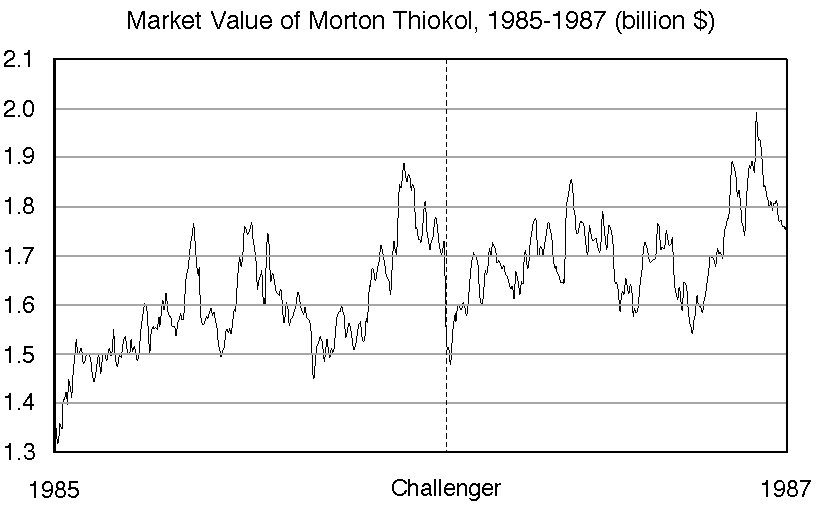
\includegraphics{thval-final}
\end{center}
\caption{Market value of Morton Thiokol for 1985, 1986.}
\label{thval}
\end{figure}

Figure~\ref{thcar} shows Morton Thiokol's cumulative abnormal returns for fifty days around the event. They are as expected. That is, they tended around zero before the accident and moved under zero after the accident.

\begin{figure}[hp]
\begin{center}
%% GNUPLOT: LaTeX picture
\setlength{\unitlength}{0.240900pt}
\ifx\plotpoint\undefined\newsavebox{\plotpoint}\fi
\sbox{\plotpoint}{\rule[-0.175pt]{0.350pt}{0.350pt}}%
\begin{picture}(1500,900)(0,0)
%\tenrm
\put(264,577){\rule[-0.175pt]{282.335pt}{0.350pt}}
\put(850,158){\rule[-0.175pt]{0.350pt}{151.526pt}}
\put(264,158){\rule[-0.175pt]{4.818pt}{0.350pt}}
\put(242,158){\makebox(0,0)[r]{-0.20}}
\put(1416,158){\rule[-0.175pt]{4.818pt}{0.350pt}}
\put(264,263){\rule[-0.175pt]{4.818pt}{0.350pt}}
\put(242,263){\makebox(0,0)[r]{-0.15}}
\put(1416,263){\rule[-0.175pt]{4.818pt}{0.350pt}}
\put(264,368){\rule[-0.175pt]{4.818pt}{0.350pt}}
\put(242,368){\makebox(0,0)[r]{-0.10}}
\put(1416,368){\rule[-0.175pt]{4.818pt}{0.350pt}}
\put(264,472){\rule[-0.175pt]{4.818pt}{0.350pt}}
\put(242,472){\makebox(0,0)[r]{-0.05}}
\put(1416,472){\rule[-0.175pt]{4.818pt}{0.350pt}}
\put(264,577){\rule[-0.175pt]{4.818pt}{0.350pt}}
\put(242,577){\makebox(0,0)[r]{0.00}}
\put(1416,577){\rule[-0.175pt]{4.818pt}{0.350pt}}
\put(264,682){\rule[-0.175pt]{4.818pt}{0.350pt}}
\put(242,682){\makebox(0,0)[r]{0.05}}
\put(1416,682){\rule[-0.175pt]{4.818pt}{0.350pt}}
\put(264,787){\rule[-0.175pt]{4.818pt}{0.350pt}}
\put(242,787){\makebox(0,0)[r]{0.10}}
\put(1416,787){\rule[-0.175pt]{4.818pt}{0.350pt}}
\put(264,158){\rule[-0.175pt]{0.350pt}{4.818pt}}
\put(264,113){\makebox(0,0){-60}}
\put(264,767){\rule[-0.175pt]{0.350pt}{4.818pt}}
\put(459,158){\rule[-0.175pt]{0.350pt}{4.818pt}}
\put(459,113){\makebox(0,0){-40}}
\put(459,767){\rule[-0.175pt]{0.350pt}{4.818pt}}
\put(655,158){\rule[-0.175pt]{0.350pt}{4.818pt}}
\put(655,113){\makebox(0,0){-20}}
\put(655,767){\rule[-0.175pt]{0.350pt}{4.818pt}}
\put(850,158){\rule[-0.175pt]{0.350pt}{4.818pt}}
\put(850,113){\makebox(0,0){  0}}
\put(850,767){\rule[-0.175pt]{0.350pt}{4.818pt}}
\put(1045,158){\rule[-0.175pt]{0.350pt}{4.818pt}}
\put(1045,113){\makebox(0,0){ 20}}
\put(1045,767){\rule[-0.175pt]{0.350pt}{4.818pt}}
\put(1241,158){\rule[-0.175pt]{0.350pt}{4.818pt}}
\put(1241,113){\makebox(0,0){ 40}}
\put(1241,767){\rule[-0.175pt]{0.350pt}{4.818pt}}
\put(1436,158){\rule[-0.175pt]{0.350pt}{4.818pt}}
\put(1436,113){\makebox(0,0){ 60}}
\put(1436,767){\rule[-0.175pt]{0.350pt}{4.818pt}}
\put(264,158){\rule[-0.175pt]{282.335pt}{0.350pt}}
\put(1436,158){\rule[-0.175pt]{0.350pt}{151.526pt}}
\put(264,787){\rule[-0.175pt]{282.335pt}{0.350pt}}
\put(45,472){\makebox(0,0)[l]{\shortstack{car}}}
\put(850,68){\makebox(0,0){Days Around Event}}
\put(850,832){\makebox(0,0){Morton Thiokol Cumulative Abnormal Returns}}
\put(264,158){\rule[-0.175pt]{0.350pt}{151.526pt}}
\put(362,558){\usebox{\plotpoint}}
\put(362,554){\rule[-0.175pt]{0.350pt}{0.776pt}}
\put(363,551){\rule[-0.175pt]{0.350pt}{0.776pt}}
\put(364,548){\rule[-0.175pt]{0.350pt}{0.776pt}}
\put(365,545){\rule[-0.175pt]{0.350pt}{0.776pt}}
\put(366,541){\rule[-0.175pt]{0.350pt}{0.776pt}}
\put(367,538){\rule[-0.175pt]{0.350pt}{0.776pt}}
\put(368,535){\rule[-0.175pt]{0.350pt}{0.776pt}}
\put(369,532){\rule[-0.175pt]{0.350pt}{0.776pt}}
\put(370,529){\rule[-0.175pt]{0.350pt}{0.776pt}}
\put(371,529){\rule[-0.175pt]{0.350pt}{0.578pt}}
\put(372,531){\rule[-0.175pt]{0.350pt}{0.578pt}}
\put(373,533){\rule[-0.175pt]{0.350pt}{0.578pt}}
\put(374,536){\rule[-0.175pt]{0.350pt}{0.578pt}}
\put(375,538){\rule[-0.175pt]{0.350pt}{0.578pt}}
\put(376,541){\rule[-0.175pt]{0.350pt}{0.578pt}}
\put(377,543){\rule[-0.175pt]{0.350pt}{0.578pt}}
\put(378,545){\rule[-0.175pt]{0.350pt}{0.578pt}}
\put(379,548){\rule[-0.175pt]{0.350pt}{0.578pt}}
\put(380,550){\rule[-0.175pt]{0.350pt}{0.578pt}}
\put(381,553){\rule[-0.175pt]{0.350pt}{0.723pt}}
\put(382,556){\rule[-0.175pt]{0.350pt}{0.723pt}}
\put(383,559){\rule[-0.175pt]{0.350pt}{0.723pt}}
\put(384,562){\rule[-0.175pt]{0.350pt}{0.723pt}}
\put(385,565){\rule[-0.175pt]{0.350pt}{0.723pt}}
\put(386,568){\rule[-0.175pt]{0.350pt}{0.723pt}}
\put(387,571){\rule[-0.175pt]{0.350pt}{0.723pt}}
\put(388,574){\rule[-0.175pt]{0.350pt}{0.723pt}}
\put(389,577){\rule[-0.175pt]{0.350pt}{0.723pt}}
\put(390,580){\rule[-0.175pt]{0.350pt}{0.723pt}}
\put(391,583){\usebox{\plotpoint}}
\put(392,584){\usebox{\plotpoint}}
\put(393,585){\usebox{\plotpoint}}
\put(394,586){\usebox{\plotpoint}}
\put(395,587){\usebox{\plotpoint}}
\put(396,588){\usebox{\plotpoint}}
\put(397,589){\usebox{\plotpoint}}
\put(398,590){\usebox{\plotpoint}}
\put(399,591){\usebox{\plotpoint}}
\put(400,592){\usebox{\plotpoint}}
\put(401,593){\rule[-0.175pt]{0.350pt}{0.578pt}}
\put(402,596){\rule[-0.175pt]{0.350pt}{0.578pt}}
\put(403,598){\rule[-0.175pt]{0.350pt}{0.578pt}}
\put(404,601){\rule[-0.175pt]{0.350pt}{0.578pt}}
\put(405,603){\rule[-0.175pt]{0.350pt}{0.578pt}}
\put(406,606){\rule[-0.175pt]{0.350pt}{0.578pt}}
\put(407,608){\rule[-0.175pt]{0.350pt}{0.578pt}}
\put(408,610){\rule[-0.175pt]{0.350pt}{0.578pt}}
\put(409,613){\rule[-0.175pt]{0.350pt}{0.578pt}}
\put(410,615){\rule[-0.175pt]{0.350pt}{0.578pt}}
\put(411,616){\rule[-0.175pt]{0.350pt}{0.482pt}}
\put(412,614){\rule[-0.175pt]{0.350pt}{0.482pt}}
\put(413,612){\rule[-0.175pt]{0.350pt}{0.482pt}}
\put(414,610){\rule[-0.175pt]{0.350pt}{0.482pt}}
\put(415,608){\rule[-0.175pt]{0.350pt}{0.482pt}}
\put(416,606){\rule[-0.175pt]{0.350pt}{0.482pt}}
\put(417,604){\rule[-0.175pt]{0.350pt}{0.482pt}}
\put(418,602){\rule[-0.175pt]{0.350pt}{0.482pt}}
\put(419,600){\rule[-0.175pt]{0.350pt}{0.482pt}}
\put(420,598){\rule[-0.175pt]{0.350pt}{0.361pt}}
\put(421,597){\rule[-0.175pt]{0.350pt}{0.361pt}}
\put(422,595){\rule[-0.175pt]{0.350pt}{0.361pt}}
\put(423,594){\rule[-0.175pt]{0.350pt}{0.361pt}}
\put(424,592){\rule[-0.175pt]{0.350pt}{0.361pt}}
\put(425,591){\rule[-0.175pt]{0.350pt}{0.361pt}}
\put(426,589){\rule[-0.175pt]{0.350pt}{0.361pt}}
\put(427,588){\rule[-0.175pt]{0.350pt}{0.361pt}}
\put(428,586){\rule[-0.175pt]{0.350pt}{0.361pt}}
\put(429,585){\rule[-0.175pt]{0.350pt}{0.361pt}}
\put(430,583){\rule[-0.175pt]{0.350pt}{0.361pt}}
\put(431,582){\rule[-0.175pt]{0.350pt}{0.361pt}}
\put(432,580){\rule[-0.175pt]{0.350pt}{0.361pt}}
\put(433,579){\rule[-0.175pt]{0.350pt}{0.361pt}}
\put(434,577){\rule[-0.175pt]{0.350pt}{0.361pt}}
\put(435,576){\rule[-0.175pt]{0.350pt}{0.361pt}}
\put(436,574){\rule[-0.175pt]{0.350pt}{0.361pt}}
\put(437,573){\rule[-0.175pt]{0.350pt}{0.361pt}}
\put(438,571){\rule[-0.175pt]{0.350pt}{0.361pt}}
\put(439,570){\rule[-0.175pt]{0.350pt}{0.361pt}}
\put(440,566){\rule[-0.175pt]{0.350pt}{0.915pt}}
\put(441,562){\rule[-0.175pt]{0.350pt}{0.915pt}}
\put(442,558){\rule[-0.175pt]{0.350pt}{0.915pt}}
\put(443,554){\rule[-0.175pt]{0.350pt}{0.915pt}}
\put(444,551){\rule[-0.175pt]{0.350pt}{0.915pt}}
\put(445,547){\rule[-0.175pt]{0.350pt}{0.915pt}}
\put(446,543){\rule[-0.175pt]{0.350pt}{0.915pt}}
\put(447,539){\rule[-0.175pt]{0.350pt}{0.915pt}}
\put(448,535){\rule[-0.175pt]{0.350pt}{0.915pt}}
\put(449,532){\rule[-0.175pt]{0.350pt}{0.915pt}}
\put(450,530){\usebox{\plotpoint}}
\put(451,529){\usebox{\plotpoint}}
\put(452,528){\usebox{\plotpoint}}
\put(453,527){\usebox{\plotpoint}}
\put(454,526){\usebox{\plotpoint}}
\put(455,525){\usebox{\plotpoint}}
\put(456,524){\usebox{\plotpoint}}
\put(457,523){\usebox{\plotpoint}}
\put(458,522){\usebox{\plotpoint}}
\put(459,522){\usebox{\plotpoint}}
\put(459,522){\rule[-0.175pt]{0.401pt}{0.350pt}}
\put(460,523){\rule[-0.175pt]{0.401pt}{0.350pt}}
\put(462,524){\rule[-0.175pt]{0.401pt}{0.350pt}}
\put(463,525){\rule[-0.175pt]{0.401pt}{0.350pt}}
\put(465,526){\rule[-0.175pt]{0.401pt}{0.350pt}}
\put(467,527){\rule[-0.175pt]{0.401pt}{0.350pt}}
\put(468,528){\usebox{\plotpoint}}
\put(469,523){\rule[-0.175pt]{0.350pt}{1.132pt}}
\put(470,518){\rule[-0.175pt]{0.350pt}{1.132pt}}
\put(471,513){\rule[-0.175pt]{0.350pt}{1.132pt}}
\put(472,509){\rule[-0.175pt]{0.350pt}{1.132pt}}
\put(473,504){\rule[-0.175pt]{0.350pt}{1.132pt}}
\put(474,499){\rule[-0.175pt]{0.350pt}{1.132pt}}
\put(475,495){\rule[-0.175pt]{0.350pt}{1.132pt}}
\put(476,490){\rule[-0.175pt]{0.350pt}{1.132pt}}
\put(477,485){\rule[-0.175pt]{0.350pt}{1.132pt}}
\put(478,481){\rule[-0.175pt]{0.350pt}{1.132pt}}
\put(479,481){\rule[-0.175pt]{0.350pt}{1.783pt}}
\put(480,488){\rule[-0.175pt]{0.350pt}{1.783pt}}
\put(481,495){\rule[-0.175pt]{0.350pt}{1.783pt}}
\put(482,503){\rule[-0.175pt]{0.350pt}{1.783pt}}
\put(483,510){\rule[-0.175pt]{0.350pt}{1.783pt}}
\put(484,518){\rule[-0.175pt]{0.350pt}{1.783pt}}
\put(485,525){\rule[-0.175pt]{0.350pt}{1.783pt}}
\put(486,532){\rule[-0.175pt]{0.350pt}{1.783pt}}
\put(487,540){\rule[-0.175pt]{0.350pt}{1.783pt}}
\put(488,547){\rule[-0.175pt]{0.350pt}{1.783pt}}
\put(489,555){\rule[-0.175pt]{0.350pt}{1.633pt}}
\put(490,561){\rule[-0.175pt]{0.350pt}{1.633pt}}
\put(491,568){\rule[-0.175pt]{0.350pt}{1.633pt}}
\put(492,575){\rule[-0.175pt]{0.350pt}{1.633pt}}
\put(493,582){\rule[-0.175pt]{0.350pt}{1.633pt}}
\put(494,588){\rule[-0.175pt]{0.350pt}{1.633pt}}
\put(495,595){\rule[-0.175pt]{0.350pt}{1.633pt}}
\put(496,602){\rule[-0.175pt]{0.350pt}{1.633pt}}
\put(497,609){\rule[-0.175pt]{0.350pt}{1.633pt}}
\put(498,615){\usebox{\plotpoint}}
\put(498,614){\usebox{\plotpoint}}
\put(499,613){\usebox{\plotpoint}}
\put(500,611){\usebox{\plotpoint}}
\put(501,610){\usebox{\plotpoint}}
\put(502,608){\usebox{\plotpoint}}
\put(503,607){\usebox{\plotpoint}}
\put(504,606){\usebox{\plotpoint}}
\put(505,604){\usebox{\plotpoint}}
\put(506,603){\usebox{\plotpoint}}
\put(507,602){\usebox{\plotpoint}}
\put(508,600){\usebox{\plotpoint}}
\put(509,599){\usebox{\plotpoint}}
\put(510,598){\usebox{\plotpoint}}
\put(511,597){\usebox{\plotpoint}}
\put(512,595){\usebox{\plotpoint}}
\put(513,594){\usebox{\plotpoint}}
\put(514,593){\usebox{\plotpoint}}
\put(515,592){\usebox{\plotpoint}}
\put(516,591){\usebox{\plotpoint}}
\put(517,590){\usebox{\plotpoint}}
\put(518,590){\rule[-0.175pt]{0.350pt}{2.650pt}}
\put(519,601){\rule[-0.175pt]{0.350pt}{2.650pt}}
\put(520,612){\rule[-0.175pt]{0.350pt}{2.650pt}}
\put(521,623){\rule[-0.175pt]{0.350pt}{2.650pt}}
\put(522,634){\rule[-0.175pt]{0.350pt}{2.650pt}}
\put(523,645){\rule[-0.175pt]{0.350pt}{2.650pt}}
\put(524,656){\rule[-0.175pt]{0.350pt}{2.650pt}}
\put(525,667){\rule[-0.175pt]{0.350pt}{2.650pt}}
\put(526,678){\rule[-0.175pt]{0.350pt}{2.650pt}}
\put(527,689){\rule[-0.175pt]{0.350pt}{2.650pt}}
\put(528,700){\rule[-0.175pt]{0.350pt}{1.740pt}}
\put(529,707){\rule[-0.175pt]{0.350pt}{1.740pt}}
\put(530,714){\rule[-0.175pt]{0.350pt}{1.740pt}}
\put(531,721){\rule[-0.175pt]{0.350pt}{1.740pt}}
\put(532,728){\rule[-0.175pt]{0.350pt}{1.740pt}}
\put(533,736){\rule[-0.175pt]{0.350pt}{1.740pt}}
\put(534,743){\rule[-0.175pt]{0.350pt}{1.740pt}}
\put(535,750){\rule[-0.175pt]{0.350pt}{1.740pt}}
\put(536,757){\rule[-0.175pt]{0.350pt}{1.740pt}}
\put(537,763){\rule[-0.175pt]{0.350pt}{0.482pt}}
\put(538,761){\rule[-0.175pt]{0.350pt}{0.482pt}}
\put(539,759){\rule[-0.175pt]{0.350pt}{0.482pt}}
\put(540,757){\rule[-0.175pt]{0.350pt}{0.482pt}}
\put(541,755){\rule[-0.175pt]{0.350pt}{0.482pt}}
\put(542,753){\rule[-0.175pt]{0.350pt}{0.482pt}}
\put(543,751){\rule[-0.175pt]{0.350pt}{0.482pt}}
\put(544,749){\rule[-0.175pt]{0.350pt}{0.482pt}}
\put(545,747){\rule[-0.175pt]{0.350pt}{0.482pt}}
\put(546,745){\rule[-0.175pt]{0.350pt}{0.482pt}}
\put(547,745){\rule[-0.175pt]{0.803pt}{0.350pt}}
\put(550,746){\rule[-0.175pt]{0.803pt}{0.350pt}}
\put(553,747){\rule[-0.175pt]{0.803pt}{0.350pt}}
\put(556,748){\usebox{\plotpoint}}
\put(557,748){\rule[-0.175pt]{0.350pt}{0.819pt}}
\put(558,751){\rule[-0.175pt]{0.350pt}{0.819pt}}
\put(559,754){\rule[-0.175pt]{0.350pt}{0.819pt}}
\put(560,758){\rule[-0.175pt]{0.350pt}{0.819pt}}
\put(561,761){\rule[-0.175pt]{0.350pt}{0.819pt}}
\put(562,765){\rule[-0.175pt]{0.350pt}{0.819pt}}
\put(563,768){\rule[-0.175pt]{0.350pt}{0.819pt}}
\put(564,771){\rule[-0.175pt]{0.350pt}{0.819pt}}
\put(565,775){\rule[-0.175pt]{0.350pt}{0.819pt}}
\put(566,778){\rule[-0.175pt]{0.350pt}{0.819pt}}
\put(567,780){\rule[-0.175pt]{0.350pt}{0.434pt}}
\put(568,778){\rule[-0.175pt]{0.350pt}{0.434pt}}
\put(569,776){\rule[-0.175pt]{0.350pt}{0.434pt}}
\put(570,774){\rule[-0.175pt]{0.350pt}{0.434pt}}
\put(571,773){\rule[-0.175pt]{0.350pt}{0.434pt}}
\put(572,771){\rule[-0.175pt]{0.350pt}{0.434pt}}
\put(573,769){\rule[-0.175pt]{0.350pt}{0.434pt}}
\put(574,767){\rule[-0.175pt]{0.350pt}{0.434pt}}
\put(575,765){\rule[-0.175pt]{0.350pt}{0.434pt}}
\put(576,764){\rule[-0.175pt]{0.350pt}{0.434pt}}
\put(577,762){\usebox{\plotpoint}}
\put(578,761){\usebox{\plotpoint}}
\put(579,760){\usebox{\plotpoint}}
\put(580,758){\usebox{\plotpoint}}
\put(581,757){\usebox{\plotpoint}}
\put(582,756){\usebox{\plotpoint}}
\put(583,754){\usebox{\plotpoint}}
\put(584,753){\usebox{\plotpoint}}
\put(585,752){\usebox{\plotpoint}}
\put(586,752){\usebox{\plotpoint}}
\put(586,752){\rule[-0.175pt]{0.350pt}{0.434pt}}
\put(587,753){\rule[-0.175pt]{0.350pt}{0.434pt}}
\put(588,755){\rule[-0.175pt]{0.350pt}{0.434pt}}
\put(589,757){\rule[-0.175pt]{0.350pt}{0.434pt}}
\put(590,759){\rule[-0.175pt]{0.350pt}{0.434pt}}
\put(591,760){\rule[-0.175pt]{0.350pt}{0.434pt}}
\put(592,762){\rule[-0.175pt]{0.350pt}{0.434pt}}
\put(593,764){\rule[-0.175pt]{0.350pt}{0.434pt}}
\put(594,766){\rule[-0.175pt]{0.350pt}{0.434pt}}
\put(595,768){\rule[-0.175pt]{0.350pt}{0.434pt}}
\put(596,769){\usebox{\plotpoint}}
\put(596,768){\usebox{\plotpoint}}
\put(597,767){\usebox{\plotpoint}}
\put(598,765){\usebox{\plotpoint}}
\put(599,764){\usebox{\plotpoint}}
\put(600,762){\usebox{\plotpoint}}
\put(601,761){\usebox{\plotpoint}}
\put(602,760){\usebox{\plotpoint}}
\put(603,758){\usebox{\plotpoint}}
\put(604,757){\usebox{\plotpoint}}
\put(605,756){\usebox{\plotpoint}}
\put(606,753){\rule[-0.175pt]{0.350pt}{0.554pt}}
\put(607,751){\rule[-0.175pt]{0.350pt}{0.554pt}}
\put(608,749){\rule[-0.175pt]{0.350pt}{0.554pt}}
\put(609,746){\rule[-0.175pt]{0.350pt}{0.554pt}}
\put(610,744){\rule[-0.175pt]{0.350pt}{0.554pt}}
\put(611,742){\rule[-0.175pt]{0.350pt}{0.554pt}}
\put(612,739){\rule[-0.175pt]{0.350pt}{0.554pt}}
\put(613,737){\rule[-0.175pt]{0.350pt}{0.554pt}}
\put(614,735){\rule[-0.175pt]{0.350pt}{0.554pt}}
\put(615,733){\rule[-0.175pt]{0.350pt}{0.554pt}}
\put(616,733){\usebox{\plotpoint}}
\put(616,733){\rule[-0.175pt]{0.350pt}{0.669pt}}
\put(617,735){\rule[-0.175pt]{0.350pt}{0.669pt}}
\put(618,738){\rule[-0.175pt]{0.350pt}{0.669pt}}
\put(619,741){\rule[-0.175pt]{0.350pt}{0.669pt}}
\put(620,744){\rule[-0.175pt]{0.350pt}{0.669pt}}
\put(621,746){\rule[-0.175pt]{0.350pt}{0.669pt}}
\put(622,749){\rule[-0.175pt]{0.350pt}{0.669pt}}
\put(623,752){\rule[-0.175pt]{0.350pt}{0.669pt}}
\put(624,755){\rule[-0.175pt]{0.350pt}{0.669pt}}
\put(625,757){\usebox{\plotpoint}}
\put(625,756){\rule[-0.175pt]{0.350pt}{0.458pt}}
\put(626,754){\rule[-0.175pt]{0.350pt}{0.458pt}}
\put(627,752){\rule[-0.175pt]{0.350pt}{0.458pt}}
\put(628,750){\rule[-0.175pt]{0.350pt}{0.458pt}}
\put(629,748){\rule[-0.175pt]{0.350pt}{0.458pt}}
\put(630,746){\rule[-0.175pt]{0.350pt}{0.458pt}}
\put(631,744){\rule[-0.175pt]{0.350pt}{0.458pt}}
\put(632,742){\rule[-0.175pt]{0.350pt}{0.458pt}}
\put(633,740){\rule[-0.175pt]{0.350pt}{0.458pt}}
\put(634,739){\rule[-0.175pt]{0.350pt}{0.458pt}}
\put(635,728){\rule[-0.175pt]{0.350pt}{2.650pt}}
\put(636,717){\rule[-0.175pt]{0.350pt}{2.650pt}}
\put(637,706){\rule[-0.175pt]{0.350pt}{2.650pt}}
\put(638,695){\rule[-0.175pt]{0.350pt}{2.650pt}}
\put(639,684){\rule[-0.175pt]{0.350pt}{2.650pt}}
\put(640,673){\rule[-0.175pt]{0.350pt}{2.650pt}}
\put(641,662){\rule[-0.175pt]{0.350pt}{2.650pt}}
\put(642,651){\rule[-0.175pt]{0.350pt}{2.650pt}}
\put(643,640){\rule[-0.175pt]{0.350pt}{2.650pt}}
\put(644,629){\rule[-0.175pt]{0.350pt}{2.650pt}}
\put(645,629){\rule[-0.175pt]{0.803pt}{0.350pt}}
\put(648,630){\rule[-0.175pt]{0.803pt}{0.350pt}}
\put(651,631){\rule[-0.175pt]{0.803pt}{0.350pt}}
\put(654,632){\usebox{\plotpoint}}
\put(655,626){\rule[-0.175pt]{0.350pt}{1.445pt}}
\put(656,620){\rule[-0.175pt]{0.350pt}{1.445pt}}
\put(657,614){\rule[-0.175pt]{0.350pt}{1.445pt}}
\put(658,608){\rule[-0.175pt]{0.350pt}{1.445pt}}
\put(659,602){\rule[-0.175pt]{0.350pt}{1.445pt}}
\put(660,596){\rule[-0.175pt]{0.350pt}{1.445pt}}
\put(661,590){\rule[-0.175pt]{0.350pt}{1.445pt}}
\put(662,584){\rule[-0.175pt]{0.350pt}{1.445pt}}
\put(663,578){\rule[-0.175pt]{0.350pt}{1.445pt}}
\put(664,578){\rule[-0.175pt]{2.409pt}{0.350pt}}
\put(674,575){\rule[-0.175pt]{0.350pt}{0.723pt}}
\put(675,572){\rule[-0.175pt]{0.350pt}{0.723pt}}
\put(676,569){\rule[-0.175pt]{0.350pt}{0.723pt}}
\put(677,566){\rule[-0.175pt]{0.350pt}{0.723pt}}
\put(678,563){\rule[-0.175pt]{0.350pt}{0.723pt}}
\put(679,560){\rule[-0.175pt]{0.350pt}{0.723pt}}
\put(680,557){\rule[-0.175pt]{0.350pt}{0.723pt}}
\put(681,554){\rule[-0.175pt]{0.350pt}{0.723pt}}
\put(682,551){\rule[-0.175pt]{0.350pt}{0.723pt}}
\put(683,548){\rule[-0.175pt]{0.350pt}{0.723pt}}
\put(684,548){\rule[-0.175pt]{0.350pt}{0.747pt}}
\put(685,551){\rule[-0.175pt]{0.350pt}{0.747pt}}
\put(686,554){\rule[-0.175pt]{0.350pt}{0.747pt}}
\put(687,557){\rule[-0.175pt]{0.350pt}{0.747pt}}
\put(688,560){\rule[-0.175pt]{0.350pt}{0.747pt}}
\put(689,563){\rule[-0.175pt]{0.350pt}{0.747pt}}
\put(690,566){\rule[-0.175pt]{0.350pt}{0.747pt}}
\put(691,569){\rule[-0.175pt]{0.350pt}{0.747pt}}
\put(692,572){\rule[-0.175pt]{0.350pt}{0.747pt}}
\put(693,575){\rule[-0.175pt]{0.350pt}{0.747pt}}
\put(694,578){\rule[-0.175pt]{0.350pt}{1.060pt}}
\put(695,583){\rule[-0.175pt]{0.350pt}{1.060pt}}
\put(696,587){\rule[-0.175pt]{0.350pt}{1.060pt}}
\put(697,592){\rule[-0.175pt]{0.350pt}{1.060pt}}
\put(698,596){\rule[-0.175pt]{0.350pt}{1.060pt}}
\put(699,601){\rule[-0.175pt]{0.350pt}{1.060pt}}
\put(700,605){\rule[-0.175pt]{0.350pt}{1.060pt}}
\put(701,609){\rule[-0.175pt]{0.350pt}{1.060pt}}
\put(702,614){\rule[-0.175pt]{0.350pt}{1.060pt}}
\put(703,618){\rule[-0.175pt]{0.350pt}{1.060pt}}
\put(704,623){\rule[-0.175pt]{0.350pt}{0.964pt}}
\put(705,627){\rule[-0.175pt]{0.350pt}{0.964pt}}
\put(706,631){\rule[-0.175pt]{0.350pt}{0.964pt}}
\put(707,635){\rule[-0.175pt]{0.350pt}{0.964pt}}
\put(708,639){\rule[-0.175pt]{0.350pt}{0.964pt}}
\put(709,643){\rule[-0.175pt]{0.350pt}{0.964pt}}
\put(710,647){\rule[-0.175pt]{0.350pt}{0.964pt}}
\put(711,651){\rule[-0.175pt]{0.350pt}{0.964pt}}
\put(712,655){\rule[-0.175pt]{0.350pt}{0.964pt}}
\put(713,655){\rule[-0.175pt]{0.350pt}{0.915pt}}
\put(714,651){\rule[-0.175pt]{0.350pt}{0.915pt}}
\put(715,647){\rule[-0.175pt]{0.350pt}{0.915pt}}
\put(716,643){\rule[-0.175pt]{0.350pt}{0.915pt}}
\put(717,640){\rule[-0.175pt]{0.350pt}{0.915pt}}
\put(718,636){\rule[-0.175pt]{0.350pt}{0.915pt}}
\put(719,632){\rule[-0.175pt]{0.350pt}{0.915pt}}
\put(720,628){\rule[-0.175pt]{0.350pt}{0.915pt}}
\put(721,624){\rule[-0.175pt]{0.350pt}{0.915pt}}
\put(722,621){\rule[-0.175pt]{0.350pt}{0.915pt}}
\put(723,619){\rule[-0.175pt]{0.350pt}{0.482pt}}
\put(724,617){\rule[-0.175pt]{0.350pt}{0.482pt}}
\put(725,615){\rule[-0.175pt]{0.350pt}{0.482pt}}
\put(726,613){\rule[-0.175pt]{0.350pt}{0.482pt}}
\put(727,611){\rule[-0.175pt]{0.350pt}{0.482pt}}
\put(728,609){\rule[-0.175pt]{0.350pt}{0.482pt}}
\put(729,607){\rule[-0.175pt]{0.350pt}{0.482pt}}
\put(730,605){\rule[-0.175pt]{0.350pt}{0.482pt}}
\put(731,603){\rule[-0.175pt]{0.350pt}{0.482pt}}
\put(732,601){\rule[-0.175pt]{0.350pt}{0.482pt}}
\put(733,597){\rule[-0.175pt]{0.350pt}{0.819pt}}
\put(734,594){\rule[-0.175pt]{0.350pt}{0.819pt}}
\put(735,590){\rule[-0.175pt]{0.350pt}{0.819pt}}
\put(736,587){\rule[-0.175pt]{0.350pt}{0.819pt}}
\put(737,583){\rule[-0.175pt]{0.350pt}{0.819pt}}
\put(738,580){\rule[-0.175pt]{0.350pt}{0.819pt}}
\put(739,577){\rule[-0.175pt]{0.350pt}{0.819pt}}
\put(740,573){\rule[-0.175pt]{0.350pt}{0.819pt}}
\put(741,570){\rule[-0.175pt]{0.350pt}{0.819pt}}
\put(742,567){\rule[-0.175pt]{0.350pt}{0.819pt}}
\put(743,567){\rule[-0.175pt]{0.350pt}{0.509pt}}
\put(744,569){\rule[-0.175pt]{0.350pt}{0.509pt}}
\put(745,571){\rule[-0.175pt]{0.350pt}{0.509pt}}
\put(746,573){\rule[-0.175pt]{0.350pt}{0.509pt}}
\put(747,575){\rule[-0.175pt]{0.350pt}{0.509pt}}
\put(748,577){\rule[-0.175pt]{0.350pt}{0.509pt}}
\put(749,579){\rule[-0.175pt]{0.350pt}{0.509pt}}
\put(750,581){\rule[-0.175pt]{0.350pt}{0.509pt}}
\put(751,583){\rule[-0.175pt]{0.350pt}{0.509pt}}
\put(752,585){\usebox{\plotpoint}}
\put(752,586){\rule[-0.175pt]{0.402pt}{0.350pt}}
\put(753,585){\rule[-0.175pt]{0.402pt}{0.350pt}}
\put(755,584){\rule[-0.175pt]{0.402pt}{0.350pt}}
\put(757,583){\rule[-0.175pt]{0.402pt}{0.350pt}}
\put(758,582){\rule[-0.175pt]{0.402pt}{0.350pt}}
\put(760,581){\rule[-0.175pt]{0.401pt}{0.350pt}}
\put(762,580){\rule[-0.175pt]{0.350pt}{0.675pt}}
\put(763,582){\rule[-0.175pt]{0.350pt}{0.675pt}}
\put(764,585){\rule[-0.175pt]{0.350pt}{0.675pt}}
\put(765,588){\rule[-0.175pt]{0.350pt}{0.675pt}}
\put(766,591){\rule[-0.175pt]{0.350pt}{0.675pt}}
\put(767,593){\rule[-0.175pt]{0.350pt}{0.675pt}}
\put(768,596){\rule[-0.175pt]{0.350pt}{0.675pt}}
\put(769,599){\rule[-0.175pt]{0.350pt}{0.675pt}}
\put(770,602){\rule[-0.175pt]{0.350pt}{0.675pt}}
\put(771,605){\rule[-0.175pt]{0.350pt}{0.675pt}}
\put(772,607){\rule[-0.175pt]{0.350pt}{0.434pt}}
\put(773,609){\rule[-0.175pt]{0.350pt}{0.434pt}}
\put(774,611){\rule[-0.175pt]{0.350pt}{0.434pt}}
\put(775,613){\rule[-0.175pt]{0.350pt}{0.434pt}}
\put(776,615){\rule[-0.175pt]{0.350pt}{0.434pt}}
\put(777,616){\rule[-0.175pt]{0.350pt}{0.434pt}}
\put(778,618){\rule[-0.175pt]{0.350pt}{0.434pt}}
\put(779,620){\rule[-0.175pt]{0.350pt}{0.434pt}}
\put(780,622){\rule[-0.175pt]{0.350pt}{0.434pt}}
\put(781,624){\rule[-0.175pt]{0.350pt}{0.434pt}}
\put(782,625){\usebox{\plotpoint}}
\put(782,623){\rule[-0.175pt]{0.350pt}{0.616pt}}
\put(783,620){\rule[-0.175pt]{0.350pt}{0.616pt}}
\put(784,618){\rule[-0.175pt]{0.350pt}{0.616pt}}
\put(785,615){\rule[-0.175pt]{0.350pt}{0.616pt}}
\put(786,613){\rule[-0.175pt]{0.350pt}{0.616pt}}
\put(787,610){\rule[-0.175pt]{0.350pt}{0.616pt}}
\put(788,608){\rule[-0.175pt]{0.350pt}{0.616pt}}
\put(789,605){\rule[-0.175pt]{0.350pt}{0.616pt}}
\put(790,603){\rule[-0.175pt]{0.350pt}{0.616pt}}
\put(791,600){\rule[-0.175pt]{0.350pt}{0.530pt}}
\put(792,598){\rule[-0.175pt]{0.350pt}{0.530pt}}
\put(793,596){\rule[-0.175pt]{0.350pt}{0.530pt}}
\put(794,594){\rule[-0.175pt]{0.350pt}{0.530pt}}
\put(795,591){\rule[-0.175pt]{0.350pt}{0.530pt}}
\put(796,589){\rule[-0.175pt]{0.350pt}{0.530pt}}
\put(797,587){\rule[-0.175pt]{0.350pt}{0.530pt}}
\put(798,585){\rule[-0.175pt]{0.350pt}{0.530pt}}
\put(799,583){\rule[-0.175pt]{0.350pt}{0.530pt}}
\put(800,581){\rule[-0.175pt]{0.350pt}{0.530pt}}
\put(801,581){\rule[-0.175pt]{0.602pt}{0.350pt}}
\put(803,580){\rule[-0.175pt]{0.602pt}{0.350pt}}
\put(806,579){\rule[-0.175pt]{0.602pt}{0.350pt}}
\put(808,578){\rule[-0.175pt]{0.602pt}{0.350pt}}
\put(811,575){\rule[-0.175pt]{0.350pt}{0.385pt}}
\put(812,573){\rule[-0.175pt]{0.350pt}{0.385pt}}
\put(813,572){\rule[-0.175pt]{0.350pt}{0.385pt}}
\put(814,570){\rule[-0.175pt]{0.350pt}{0.385pt}}
\put(815,569){\rule[-0.175pt]{0.350pt}{0.385pt}}
\put(816,567){\rule[-0.175pt]{0.350pt}{0.385pt}}
\put(817,565){\rule[-0.175pt]{0.350pt}{0.385pt}}
\put(818,564){\rule[-0.175pt]{0.350pt}{0.385pt}}
\put(819,562){\rule[-0.175pt]{0.350pt}{0.385pt}}
\put(820,561){\rule[-0.175pt]{0.350pt}{0.385pt}}
\put(821,561){\usebox{\plotpoint}}
\put(821,561){\usebox{\plotpoint}}
\put(822,562){\usebox{\plotpoint}}
\put(823,563){\usebox{\plotpoint}}
\put(824,564){\usebox{\plotpoint}}
\put(826,565){\usebox{\plotpoint}}
\put(827,566){\usebox{\plotpoint}}
\put(828,567){\usebox{\plotpoint}}
\put(829,568){\usebox{\plotpoint}}
\put(830,568){\rule[-0.175pt]{0.350pt}{0.482pt}}
\put(831,570){\rule[-0.175pt]{0.350pt}{0.482pt}}
\put(832,572){\rule[-0.175pt]{0.350pt}{0.482pt}}
\put(833,574){\rule[-0.175pt]{0.350pt}{0.482pt}}
\put(834,576){\rule[-0.175pt]{0.350pt}{0.482pt}}
\put(835,578){\rule[-0.175pt]{0.350pt}{0.482pt}}
\put(836,580){\rule[-0.175pt]{0.350pt}{0.482pt}}
\put(837,582){\rule[-0.175pt]{0.350pt}{0.482pt}}
\put(838,584){\rule[-0.175pt]{0.350pt}{0.482pt}}
\put(839,586){\rule[-0.175pt]{0.350pt}{0.482pt}}
\put(840,562){\rule[-0.175pt]{0.350pt}{6.119pt}}
\put(841,537){\rule[-0.175pt]{0.350pt}{6.119pt}}
\put(842,511){\rule[-0.175pt]{0.350pt}{6.119pt}}
\put(843,486){\rule[-0.175pt]{0.350pt}{6.119pt}}
\put(844,460){\rule[-0.175pt]{0.350pt}{6.119pt}}
\put(845,435){\rule[-0.175pt]{0.350pt}{6.119pt}}
\put(846,410){\rule[-0.175pt]{0.350pt}{6.119pt}}
\put(847,384){\rule[-0.175pt]{0.350pt}{6.119pt}}
\put(848,359){\rule[-0.175pt]{0.350pt}{6.119pt}}
\put(849,334){\rule[-0.175pt]{0.350pt}{6.119pt}}
\put(850,332){\rule[-0.175pt]{0.350pt}{0.434pt}}
\put(851,330){\rule[-0.175pt]{0.350pt}{0.434pt}}
\put(852,328){\rule[-0.175pt]{0.350pt}{0.434pt}}
\put(853,326){\rule[-0.175pt]{0.350pt}{0.434pt}}
\put(854,325){\rule[-0.175pt]{0.350pt}{0.434pt}}
\put(855,323){\rule[-0.175pt]{0.350pt}{0.434pt}}
\put(856,321){\rule[-0.175pt]{0.350pt}{0.434pt}}
\put(857,319){\rule[-0.175pt]{0.350pt}{0.434pt}}
\put(858,317){\rule[-0.175pt]{0.350pt}{0.434pt}}
\put(859,316){\rule[-0.175pt]{0.350pt}{0.434pt}}
\put(860,316){\usebox{\plotpoint}}
\put(860,316){\usebox{\plotpoint}}
\put(861,317){\usebox{\plotpoint}}
\put(862,318){\usebox{\plotpoint}}
\put(863,319){\usebox{\plotpoint}}
\put(864,321){\usebox{\plotpoint}}
\put(865,322){\usebox{\plotpoint}}
\put(866,323){\usebox{\plotpoint}}
\put(867,325){\usebox{\plotpoint}}
\put(868,326){\usebox{\plotpoint}}
\put(869,327){\usebox{\plotpoint}}
\put(870,328){\usebox{\plotpoint}}
\put(870,320){\rule[-0.175pt]{0.350pt}{2.115pt}}
\put(871,311){\rule[-0.175pt]{0.350pt}{2.115pt}}
\put(872,302){\rule[-0.175pt]{0.350pt}{2.115pt}}
\put(873,293){\rule[-0.175pt]{0.350pt}{2.115pt}}
\put(874,285){\rule[-0.175pt]{0.350pt}{2.115pt}}
\put(875,276){\rule[-0.175pt]{0.350pt}{2.115pt}}
\put(876,267){\rule[-0.175pt]{0.350pt}{2.115pt}}
\put(877,258){\rule[-0.175pt]{0.350pt}{2.115pt}}
\put(878,250){\rule[-0.175pt]{0.350pt}{2.115pt}}
\put(879,250){\usebox{\plotpoint}}
\put(879,250){\rule[-0.175pt]{0.350pt}{1.421pt}}
\put(880,255){\rule[-0.175pt]{0.350pt}{1.421pt}}
\put(881,261){\rule[-0.175pt]{0.350pt}{1.421pt}}
\put(882,267){\rule[-0.175pt]{0.350pt}{1.421pt}}
\put(883,273){\rule[-0.175pt]{0.350pt}{1.421pt}}
\put(884,279){\rule[-0.175pt]{0.350pt}{1.421pt}}
\put(885,285){\rule[-0.175pt]{0.350pt}{1.421pt}}
\put(886,291){\rule[-0.175pt]{0.350pt}{1.421pt}}
\put(887,297){\rule[-0.175pt]{0.350pt}{1.421pt}}
\put(888,303){\rule[-0.175pt]{0.350pt}{1.421pt}}
\put(889,308){\rule[-0.175pt]{0.350pt}{1.470pt}}
\put(890,315){\rule[-0.175pt]{0.350pt}{1.469pt}}
\put(891,321){\rule[-0.175pt]{0.350pt}{1.469pt}}
\put(892,327){\rule[-0.175pt]{0.350pt}{1.469pt}}
\put(893,333){\rule[-0.175pt]{0.350pt}{1.469pt}}
\put(894,339){\rule[-0.175pt]{0.350pt}{1.469pt}}
\put(895,345){\rule[-0.175pt]{0.350pt}{1.469pt}}
\put(896,351){\rule[-0.175pt]{0.350pt}{1.469pt}}
\put(897,357){\rule[-0.175pt]{0.350pt}{1.469pt}}
\put(898,363){\rule[-0.175pt]{0.350pt}{1.469pt}}
\put(899,370){\rule[-0.175pt]{0.350pt}{1.060pt}}
\put(900,374){\rule[-0.175pt]{0.350pt}{1.060pt}}
\put(901,378){\rule[-0.175pt]{0.350pt}{1.060pt}}
\put(902,383){\rule[-0.175pt]{0.350pt}{1.060pt}}
\put(903,387){\rule[-0.175pt]{0.350pt}{1.060pt}}
\put(904,391){\rule[-0.175pt]{0.350pt}{1.060pt}}
\put(905,396){\rule[-0.175pt]{0.350pt}{1.060pt}}
\put(906,400){\rule[-0.175pt]{0.350pt}{1.060pt}}
\put(907,405){\rule[-0.175pt]{0.350pt}{1.060pt}}
\put(908,409){\rule[-0.175pt]{0.350pt}{1.060pt}}
\put(909,413){\usebox{\plotpoint}}
\put(909,409){\rule[-0.175pt]{0.350pt}{1.017pt}}
\put(910,405){\rule[-0.175pt]{0.350pt}{1.017pt}}
\put(911,401){\rule[-0.175pt]{0.350pt}{1.017pt}}
\put(912,397){\rule[-0.175pt]{0.350pt}{1.017pt}}
\put(913,392){\rule[-0.175pt]{0.350pt}{1.017pt}}
\put(914,388){\rule[-0.175pt]{0.350pt}{1.017pt}}
\put(915,384){\rule[-0.175pt]{0.350pt}{1.017pt}}
\put(916,380){\rule[-0.175pt]{0.350pt}{1.017pt}}
\put(917,376){\rule[-0.175pt]{0.350pt}{1.017pt}}
\put(918,376){\rule[-0.175pt]{0.350pt}{1.036pt}}
\put(919,380){\rule[-0.175pt]{0.350pt}{1.036pt}}
\put(920,384){\rule[-0.175pt]{0.350pt}{1.036pt}}
\put(921,388){\rule[-0.175pt]{0.350pt}{1.036pt}}
\put(922,393){\rule[-0.175pt]{0.350pt}{1.036pt}}
\put(923,397){\rule[-0.175pt]{0.350pt}{1.036pt}}
\put(924,401){\rule[-0.175pt]{0.350pt}{1.036pt}}
\put(925,406){\rule[-0.175pt]{0.350pt}{1.036pt}}
\put(926,410){\rule[-0.175pt]{0.350pt}{1.036pt}}
\put(927,414){\rule[-0.175pt]{0.350pt}{1.036pt}}
\put(928,418){\usebox{\plotpoint}}
\put(928,419){\rule[-0.175pt]{0.402pt}{0.350pt}}
\put(929,418){\rule[-0.175pt]{0.402pt}{0.350pt}}
\put(931,417){\rule[-0.175pt]{0.402pt}{0.350pt}}
\put(933,416){\rule[-0.175pt]{0.402pt}{0.350pt}}
\put(934,415){\rule[-0.175pt]{0.402pt}{0.350pt}}
\put(936,414){\rule[-0.175pt]{0.401pt}{0.350pt}}
\put(938,411){\rule[-0.175pt]{0.350pt}{0.361pt}}
\put(939,410){\rule[-0.175pt]{0.350pt}{0.361pt}}
\put(940,408){\rule[-0.175pt]{0.350pt}{0.361pt}}
\put(941,407){\rule[-0.175pt]{0.350pt}{0.361pt}}
\put(942,405){\rule[-0.175pt]{0.350pt}{0.361pt}}
\put(943,404){\rule[-0.175pt]{0.350pt}{0.361pt}}
\put(944,402){\rule[-0.175pt]{0.350pt}{0.361pt}}
\put(945,401){\rule[-0.175pt]{0.350pt}{0.361pt}}
\put(946,399){\rule[-0.175pt]{0.350pt}{0.361pt}}
\put(947,398){\rule[-0.175pt]{0.350pt}{0.361pt}}
\put(948,398){\rule[-0.175pt]{0.542pt}{0.350pt}}
\put(950,397){\rule[-0.175pt]{0.542pt}{0.350pt}}
\put(952,396){\rule[-0.175pt]{0.542pt}{0.350pt}}
\put(954,395){\rule[-0.175pt]{0.542pt}{0.350pt}}
\put(957,394){\rule[-0.175pt]{0.350pt}{0.385pt}}
\put(958,395){\rule[-0.175pt]{0.350pt}{0.385pt}}
\put(959,397){\rule[-0.175pt]{0.350pt}{0.385pt}}
\put(960,398){\rule[-0.175pt]{0.350pt}{0.385pt}}
\put(961,400){\rule[-0.175pt]{0.350pt}{0.385pt}}
\put(962,402){\rule[-0.175pt]{0.350pt}{0.385pt}}
\put(963,403){\rule[-0.175pt]{0.350pt}{0.385pt}}
\put(964,405){\rule[-0.175pt]{0.350pt}{0.385pt}}
\put(965,406){\rule[-0.175pt]{0.350pt}{0.385pt}}
\put(966,408){\rule[-0.175pt]{0.350pt}{0.385pt}}
\put(967,408){\usebox{\plotpoint}}
\put(968,407){\usebox{\plotpoint}}
\put(969,405){\usebox{\plotpoint}}
\put(970,404){\usebox{\plotpoint}}
\put(971,403){\usebox{\plotpoint}}
\put(972,401){\usebox{\plotpoint}}
\put(973,400){\usebox{\plotpoint}}
\put(974,398){\usebox{\plotpoint}}
\put(975,397){\usebox{\plotpoint}}
\put(976,396){\usebox{\plotpoint}}
\put(977,392){\rule[-0.175pt]{0.350pt}{0.915pt}}
\put(978,388){\rule[-0.175pt]{0.350pt}{0.915pt}}
\put(979,384){\rule[-0.175pt]{0.350pt}{0.915pt}}
\put(980,380){\rule[-0.175pt]{0.350pt}{0.915pt}}
\put(981,377){\rule[-0.175pt]{0.350pt}{0.915pt}}
\put(982,373){\rule[-0.175pt]{0.350pt}{0.915pt}}
\put(983,369){\rule[-0.175pt]{0.350pt}{0.915pt}}
\put(984,365){\rule[-0.175pt]{0.350pt}{0.915pt}}
\put(985,361){\rule[-0.175pt]{0.350pt}{0.915pt}}
\put(986,358){\rule[-0.175pt]{0.350pt}{0.915pt}}
\put(987,358){\usebox{\plotpoint}}
\put(987,358){\rule[-0.175pt]{0.350pt}{0.434pt}}
\put(988,359){\rule[-0.175pt]{0.350pt}{0.434pt}}
\put(989,361){\rule[-0.175pt]{0.350pt}{0.434pt}}
\put(990,363){\rule[-0.175pt]{0.350pt}{0.434pt}}
\put(991,365){\rule[-0.175pt]{0.350pt}{0.434pt}}
\put(992,366){\rule[-0.175pt]{0.350pt}{0.434pt}}
\put(993,368){\rule[-0.175pt]{0.350pt}{0.434pt}}
\put(994,370){\rule[-0.175pt]{0.350pt}{0.434pt}}
\put(995,372){\rule[-0.175pt]{0.350pt}{0.434pt}}
\put(996,374){\rule[-0.175pt]{0.350pt}{0.434pt}}
\put(997,375){\rule[-0.175pt]{0.350pt}{1.579pt}}
\put(998,382){\rule[-0.175pt]{0.350pt}{1.579pt}}
\put(999,389){\rule[-0.175pt]{0.350pt}{1.579pt}}
\put(1000,395){\rule[-0.175pt]{0.350pt}{1.579pt}}
\put(1001,402){\rule[-0.175pt]{0.350pt}{1.579pt}}
\put(1002,408){\rule[-0.175pt]{0.350pt}{1.579pt}}
\put(1003,415){\rule[-0.175pt]{0.350pt}{1.579pt}}
\put(1004,421){\rule[-0.175pt]{0.350pt}{1.579pt}}
\put(1005,428){\rule[-0.175pt]{0.350pt}{1.579pt}}
\put(1006,434){\rule[-0.175pt]{0.350pt}{0.482pt}}
\put(1007,437){\rule[-0.175pt]{0.350pt}{0.482pt}}
\put(1008,439){\rule[-0.175pt]{0.350pt}{0.482pt}}
\put(1009,441){\rule[-0.175pt]{0.350pt}{0.482pt}}
\put(1010,443){\rule[-0.175pt]{0.350pt}{0.482pt}}
\put(1011,445){\rule[-0.175pt]{0.350pt}{0.482pt}}
\put(1012,447){\rule[-0.175pt]{0.350pt}{0.482pt}}
\put(1013,449){\rule[-0.175pt]{0.350pt}{0.482pt}}
\put(1014,451){\rule[-0.175pt]{0.350pt}{0.482pt}}
\put(1015,453){\rule[-0.175pt]{0.350pt}{0.482pt}}
\put(1016,455){\rule[-0.175pt]{0.350pt}{0.723pt}}
\put(1017,458){\rule[-0.175pt]{0.350pt}{0.723pt}}
\put(1018,461){\rule[-0.175pt]{0.350pt}{0.723pt}}
\put(1019,464){\rule[-0.175pt]{0.350pt}{0.723pt}}
\put(1020,467){\rule[-0.175pt]{0.350pt}{0.723pt}}
\put(1021,470){\rule[-0.175pt]{0.350pt}{0.723pt}}
\put(1022,473){\rule[-0.175pt]{0.350pt}{0.723pt}}
\put(1023,476){\rule[-0.175pt]{0.350pt}{0.723pt}}
\put(1024,479){\rule[-0.175pt]{0.350pt}{0.723pt}}
\put(1025,482){\rule[-0.175pt]{0.350pt}{0.723pt}}
\put(1026,485){\rule[-0.175pt]{0.350pt}{0.482pt}}
\put(1027,487){\rule[-0.175pt]{0.350pt}{0.482pt}}
\put(1028,489){\rule[-0.175pt]{0.350pt}{0.482pt}}
\put(1029,491){\rule[-0.175pt]{0.350pt}{0.482pt}}
\put(1030,493){\rule[-0.175pt]{0.350pt}{0.482pt}}
\put(1031,495){\rule[-0.175pt]{0.350pt}{0.482pt}}
\put(1032,497){\rule[-0.175pt]{0.350pt}{0.482pt}}
\put(1033,499){\rule[-0.175pt]{0.350pt}{0.482pt}}
\put(1034,501){\rule[-0.175pt]{0.350pt}{0.482pt}}
\put(1035,503){\rule[-0.175pt]{0.350pt}{0.482pt}}
\put(1036,502){\rule[-0.175pt]{0.350pt}{0.535pt}}
\put(1037,500){\rule[-0.175pt]{0.350pt}{0.535pt}}
\put(1038,498){\rule[-0.175pt]{0.350pt}{0.535pt}}
\put(1039,496){\rule[-0.175pt]{0.350pt}{0.535pt}}
\put(1040,493){\rule[-0.175pt]{0.350pt}{0.535pt}}
\put(1041,491){\rule[-0.175pt]{0.350pt}{0.535pt}}
\put(1042,489){\rule[-0.175pt]{0.350pt}{0.535pt}}
\put(1043,487){\rule[-0.175pt]{0.350pt}{0.535pt}}
\put(1044,485){\rule[-0.175pt]{0.350pt}{0.535pt}}
\put(1045,482){\rule[-0.175pt]{0.350pt}{0.578pt}}
\put(1046,480){\rule[-0.175pt]{0.350pt}{0.578pt}}
\put(1047,477){\rule[-0.175pt]{0.350pt}{0.578pt}}
\put(1048,475){\rule[-0.175pt]{0.350pt}{0.578pt}}
\put(1049,473){\rule[-0.175pt]{0.350pt}{0.578pt}}
\put(1050,470){\rule[-0.175pt]{0.350pt}{0.578pt}}
\put(1051,468){\rule[-0.175pt]{0.350pt}{0.578pt}}
\put(1052,465){\rule[-0.175pt]{0.350pt}{0.578pt}}
\put(1053,463){\rule[-0.175pt]{0.350pt}{0.578pt}}
\put(1054,461){\rule[-0.175pt]{0.350pt}{0.578pt}}
\put(1055,459){\usebox{\plotpoint}}
\put(1056,458){\usebox{\plotpoint}}
\put(1057,456){\usebox{\plotpoint}}
\put(1058,455){\usebox{\plotpoint}}
\put(1059,454){\usebox{\plotpoint}}
\put(1060,452){\usebox{\plotpoint}}
\put(1061,451){\usebox{\plotpoint}}
\put(1062,449){\usebox{\plotpoint}}
\put(1063,448){\usebox{\plotpoint}}
\put(1064,447){\usebox{\plotpoint}}
\put(1065,438){\rule[-0.175pt]{0.350pt}{2.048pt}}
\put(1066,430){\rule[-0.175pt]{0.350pt}{2.048pt}}
\put(1067,421){\rule[-0.175pt]{0.350pt}{2.048pt}}
\put(1068,413){\rule[-0.175pt]{0.350pt}{2.048pt}}
\put(1069,404){\rule[-0.175pt]{0.350pt}{2.048pt}}
\put(1070,396){\rule[-0.175pt]{0.350pt}{2.048pt}}
\put(1071,387){\rule[-0.175pt]{0.350pt}{2.048pt}}
\put(1072,379){\rule[-0.175pt]{0.350pt}{2.048pt}}
\put(1073,370){\rule[-0.175pt]{0.350pt}{2.048pt}}
\put(1074,362){\rule[-0.175pt]{0.350pt}{2.048pt}}
\put(1075,358){\rule[-0.175pt]{0.350pt}{0.830pt}}
\put(1076,355){\rule[-0.175pt]{0.350pt}{0.830pt}}
\put(1077,351){\rule[-0.175pt]{0.350pt}{0.830pt}}
\put(1078,348){\rule[-0.175pt]{0.350pt}{0.830pt}}
\put(1079,344){\rule[-0.175pt]{0.350pt}{0.830pt}}
\put(1080,341){\rule[-0.175pt]{0.350pt}{0.830pt}}
\put(1081,337){\rule[-0.175pt]{0.350pt}{0.830pt}}
\put(1082,334){\rule[-0.175pt]{0.350pt}{0.830pt}}
\put(1083,331){\rule[-0.175pt]{0.350pt}{0.830pt}}
\put(1084,331){\rule[-0.175pt]{2.409pt}{0.350pt}}
\put(1094,331){\rule[-0.175pt]{0.350pt}{0.434pt}}
\put(1095,332){\rule[-0.175pt]{0.350pt}{0.434pt}}
\put(1096,334){\rule[-0.175pt]{0.350pt}{0.434pt}}
\put(1097,336){\rule[-0.175pt]{0.350pt}{0.434pt}}
\put(1098,338){\rule[-0.175pt]{0.350pt}{0.434pt}}
\put(1099,339){\rule[-0.175pt]{0.350pt}{0.434pt}}
\put(1100,341){\rule[-0.175pt]{0.350pt}{0.434pt}}
\put(1101,343){\rule[-0.175pt]{0.350pt}{0.434pt}}
\put(1102,345){\rule[-0.175pt]{0.350pt}{0.434pt}}
\put(1103,347){\rule[-0.175pt]{0.350pt}{0.434pt}}
\put(1104,348){\rule[-0.175pt]{0.350pt}{1.325pt}}
\put(1105,354){\rule[-0.175pt]{0.350pt}{1.325pt}}
\put(1106,360){\rule[-0.175pt]{0.350pt}{1.325pt}}
\put(1107,365){\rule[-0.175pt]{0.350pt}{1.325pt}}
\put(1108,371){\rule[-0.175pt]{0.350pt}{1.325pt}}
\put(1109,376){\rule[-0.175pt]{0.350pt}{1.325pt}}
\put(1110,382){\rule[-0.175pt]{0.350pt}{1.325pt}}
\put(1111,387){\rule[-0.175pt]{0.350pt}{1.325pt}}
\put(1112,393){\rule[-0.175pt]{0.350pt}{1.325pt}}
\put(1113,398){\rule[-0.175pt]{0.350pt}{1.325pt}}
\put(1114,401){\rule[-0.175pt]{0.350pt}{0.669pt}}
\put(1115,398){\rule[-0.175pt]{0.350pt}{0.669pt}}
\put(1116,395){\rule[-0.175pt]{0.350pt}{0.669pt}}
\put(1117,392){\rule[-0.175pt]{0.350pt}{0.669pt}}
\put(1118,390){\rule[-0.175pt]{0.350pt}{0.669pt}}
\put(1119,387){\rule[-0.175pt]{0.350pt}{0.669pt}}
\put(1120,384){\rule[-0.175pt]{0.350pt}{0.669pt}}
\put(1121,381){\rule[-0.175pt]{0.350pt}{0.669pt}}
\put(1122,379){\rule[-0.175pt]{0.350pt}{0.669pt}}
\put(1123,379){\usebox{\plotpoint}}
\put(1123,379){\rule[-0.175pt]{0.401pt}{0.350pt}}
\put(1124,378){\rule[-0.175pt]{0.401pt}{0.350pt}}
\put(1126,377){\rule[-0.175pt]{0.401pt}{0.350pt}}
\put(1127,376){\rule[-0.175pt]{0.401pt}{0.350pt}}
\put(1129,375){\rule[-0.175pt]{0.401pt}{0.350pt}}
\put(1131,374){\rule[-0.175pt]{0.401pt}{0.350pt}}
\put(1132,373){\usebox{\plotpoint}}
\put(1133,373){\rule[-0.175pt]{0.350pt}{0.915pt}}
\put(1134,376){\rule[-0.175pt]{0.350pt}{0.915pt}}
\put(1135,380){\rule[-0.175pt]{0.350pt}{0.915pt}}
\put(1136,384){\rule[-0.175pt]{0.350pt}{0.915pt}}
\put(1137,388){\rule[-0.175pt]{0.350pt}{0.915pt}}
\put(1138,391){\rule[-0.175pt]{0.350pt}{0.915pt}}
\put(1139,395){\rule[-0.175pt]{0.350pt}{0.915pt}}
\put(1140,399){\rule[-0.175pt]{0.350pt}{0.915pt}}
\put(1141,403){\rule[-0.175pt]{0.350pt}{0.915pt}}
\put(1142,407){\rule[-0.175pt]{0.350pt}{0.915pt}}
\put(1143,410){\usebox{\plotpoint}}
\put(1143,407){\rule[-0.175pt]{0.350pt}{0.747pt}}
\put(1144,404){\rule[-0.175pt]{0.350pt}{0.747pt}}
\put(1145,401){\rule[-0.175pt]{0.350pt}{0.747pt}}
\put(1146,398){\rule[-0.175pt]{0.350pt}{0.747pt}}
\put(1147,395){\rule[-0.175pt]{0.350pt}{0.747pt}}
\put(1148,392){\rule[-0.175pt]{0.350pt}{0.747pt}}
\put(1149,389){\rule[-0.175pt]{0.350pt}{0.747pt}}
\put(1150,386){\rule[-0.175pt]{0.350pt}{0.747pt}}
\put(1151,383){\rule[-0.175pt]{0.350pt}{0.747pt}}
\put(1152,380){\rule[-0.175pt]{0.350pt}{0.747pt}}
\put(1153,380){\rule[-0.175pt]{0.350pt}{0.819pt}}
\put(1154,383){\rule[-0.175pt]{0.350pt}{0.819pt}}
\put(1155,386){\rule[-0.175pt]{0.350pt}{0.819pt}}
\put(1156,390){\rule[-0.175pt]{0.350pt}{0.819pt}}
\put(1157,393){\rule[-0.175pt]{0.350pt}{0.819pt}}
\put(1158,396){\rule[-0.175pt]{0.350pt}{0.819pt}}
\put(1159,400){\rule[-0.175pt]{0.350pt}{0.819pt}}
\put(1160,403){\rule[-0.175pt]{0.350pt}{0.819pt}}
\put(1161,407){\rule[-0.175pt]{0.350pt}{0.819pt}}
\put(1162,410){\rule[-0.175pt]{0.350pt}{0.819pt}}
\put(1163,413){\usebox{\plotpoint}}
\put(1163,414){\rule[-0.175pt]{0.723pt}{0.350pt}}
\put(1166,415){\rule[-0.175pt]{0.723pt}{0.350pt}}
\put(1169,416){\rule[-0.175pt]{0.723pt}{0.350pt}}
\put(1172,415){\usebox{\plotpoint}}
\put(1173,414){\usebox{\plotpoint}}
\put(1174,413){\usebox{\plotpoint}}
\put(1175,412){\usebox{\plotpoint}}
\put(1176,411){\usebox{\plotpoint}}
\put(1177,410){\usebox{\plotpoint}}
\put(1178,409){\usebox{\plotpoint}}
\put(1179,408){\usebox{\plotpoint}}
\put(1180,407){\usebox{\plotpoint}}
\put(1181,406){\usebox{\plotpoint}}
\put(1182,402){\rule[-0.175pt]{0.350pt}{0.915pt}}
\put(1183,398){\rule[-0.175pt]{0.350pt}{0.915pt}}
\put(1184,394){\rule[-0.175pt]{0.350pt}{0.915pt}}
\put(1185,390){\rule[-0.175pt]{0.350pt}{0.915pt}}
\put(1186,387){\rule[-0.175pt]{0.350pt}{0.915pt}}
\put(1187,383){\rule[-0.175pt]{0.350pt}{0.915pt}}
\put(1188,379){\rule[-0.175pt]{0.350pt}{0.915pt}}
\put(1189,375){\rule[-0.175pt]{0.350pt}{0.915pt}}
\put(1190,371){\rule[-0.175pt]{0.350pt}{0.915pt}}
\put(1191,368){\rule[-0.175pt]{0.350pt}{0.915pt}}
\put(1192,368){\usebox{\plotpoint}}
\put(1192,368){\rule[-0.175pt]{2.409pt}{0.350pt}}
\put(1202,367){\rule[-0.175pt]{0.350pt}{0.401pt}}
\put(1203,365){\rule[-0.175pt]{0.350pt}{0.401pt}}
\put(1204,364){\rule[-0.175pt]{0.350pt}{0.401pt}}
\put(1205,362){\rule[-0.175pt]{0.350pt}{0.401pt}}
\put(1206,360){\rule[-0.175pt]{0.350pt}{0.401pt}}
\put(1207,359){\rule[-0.175pt]{0.350pt}{0.401pt}}
\put(1208,357){\rule[-0.175pt]{0.350pt}{0.401pt}}
\put(1209,355){\rule[-0.175pt]{0.350pt}{0.401pt}}
\put(1210,354){\rule[-0.175pt]{0.350pt}{0.401pt}}
\put(1211,354){\usebox{\plotpoint}}
\put(1211,354){\rule[-0.175pt]{2.409pt}{0.350pt}}
\put(1221,353){\rule[-0.175pt]{2.409pt}{0.350pt}}
\put(1231,354){\rule[-0.175pt]{1.204pt}{0.350pt}}
\put(1236,355){\rule[-0.175pt]{1.204pt}{0.350pt}}
\put(1241,351){\rule[-0.175pt]{0.350pt}{1.071pt}}
\put(1242,347){\rule[-0.175pt]{0.350pt}{1.071pt}}
\put(1243,342){\rule[-0.175pt]{0.350pt}{1.071pt}}
\put(1244,338){\rule[-0.175pt]{0.350pt}{1.071pt}}
\put(1245,333){\rule[-0.175pt]{0.350pt}{1.071pt}}
\put(1246,329){\rule[-0.175pt]{0.350pt}{1.071pt}}
\put(1247,324){\rule[-0.175pt]{0.350pt}{1.071pt}}
\put(1248,320){\rule[-0.175pt]{0.350pt}{1.071pt}}
\put(1249,316){\rule[-0.175pt]{0.350pt}{1.071pt}}
\put(1250,316){\rule[-0.175pt]{0.482pt}{0.350pt}}
\put(1252,317){\rule[-0.175pt]{0.482pt}{0.350pt}}
\put(1254,318){\rule[-0.175pt]{0.482pt}{0.350pt}}
\put(1256,319){\rule[-0.175pt]{0.482pt}{0.350pt}}
\put(1258,320){\rule[-0.175pt]{0.482pt}{0.350pt}}
\put(1260,321){\usebox{\plotpoint}}
\put(1261,322){\usebox{\plotpoint}}
\put(1262,323){\usebox{\plotpoint}}
\put(1263,324){\usebox{\plotpoint}}
\put(1264,325){\usebox{\plotpoint}}
\put(1265,327){\usebox{\plotpoint}}
\put(1266,328){\usebox{\plotpoint}}
\put(1267,329){\usebox{\plotpoint}}
\put(1268,330){\usebox{\plotpoint}}
\put(1269,331){\usebox{\plotpoint}}
\put(1270,330){\rule[-0.175pt]{0.350pt}{0.506pt}}
\put(1271,328){\rule[-0.175pt]{0.350pt}{0.506pt}}
\put(1272,326){\rule[-0.175pt]{0.350pt}{0.506pt}}
\put(1273,324){\rule[-0.175pt]{0.350pt}{0.506pt}}
\put(1274,322){\rule[-0.175pt]{0.350pt}{0.506pt}}
\put(1275,320){\rule[-0.175pt]{0.350pt}{0.506pt}}
\put(1276,318){\rule[-0.175pt]{0.350pt}{0.506pt}}
\put(1277,316){\rule[-0.175pt]{0.350pt}{0.506pt}}
\put(1278,314){\rule[-0.175pt]{0.350pt}{0.506pt}}
\put(1279,312){\rule[-0.175pt]{0.350pt}{0.506pt}}
\put(1280,312){\usebox{\plotpoint}}
\put(1281,313){\usebox{\plotpoint}}
\put(1282,314){\usebox{\plotpoint}}
\put(1283,315){\usebox{\plotpoint}}
\put(1285,316){\usebox{\plotpoint}}
\put(1286,317){\usebox{\plotpoint}}
\put(1287,318){\usebox{\plotpoint}}
\put(1288,319){\usebox{\plotpoint}}
\put(1290,320){\rule[-0.175pt]{0.350pt}{0.964pt}}
\put(1291,324){\rule[-0.175pt]{0.350pt}{0.964pt}}
\put(1292,328){\rule[-0.175pt]{0.350pt}{0.964pt}}
\put(1293,332){\rule[-0.175pt]{0.350pt}{0.964pt}}
\put(1294,336){\rule[-0.175pt]{0.350pt}{0.964pt}}
\put(1295,340){\rule[-0.175pt]{0.350pt}{0.964pt}}
\put(1296,344){\rule[-0.175pt]{0.350pt}{0.964pt}}
\put(1297,348){\rule[-0.175pt]{0.350pt}{0.964pt}}
\put(1298,352){\rule[-0.175pt]{0.350pt}{0.964pt}}
\put(1299,352){\rule[-0.175pt]{0.350pt}{0.843pt}}
\put(1300,349){\rule[-0.175pt]{0.350pt}{0.843pt}}
\put(1301,345){\rule[-0.175pt]{0.350pt}{0.843pt}}
\put(1302,342){\rule[-0.175pt]{0.350pt}{0.843pt}}
\put(1303,338){\rule[-0.175pt]{0.350pt}{0.843pt}}
\put(1304,335){\rule[-0.175pt]{0.350pt}{0.843pt}}
\put(1305,331){\rule[-0.175pt]{0.350pt}{0.843pt}}
\put(1306,328){\rule[-0.175pt]{0.350pt}{0.843pt}}
\put(1307,324){\rule[-0.175pt]{0.350pt}{0.843pt}}
\put(1308,321){\rule[-0.175pt]{0.350pt}{0.843pt}}
\put(1309,321){\rule[-0.175pt]{0.350pt}{1.325pt}}
\put(1310,326){\rule[-0.175pt]{0.350pt}{1.325pt}}
\put(1311,332){\rule[-0.175pt]{0.350pt}{1.325pt}}
\put(1312,337){\rule[-0.175pt]{0.350pt}{1.325pt}}
\put(1313,343){\rule[-0.175pt]{0.350pt}{1.325pt}}
\put(1314,348){\rule[-0.175pt]{0.350pt}{1.325pt}}
\put(1315,354){\rule[-0.175pt]{0.350pt}{1.325pt}}
\put(1316,359){\rule[-0.175pt]{0.350pt}{1.325pt}}
\put(1317,365){\rule[-0.175pt]{0.350pt}{1.325pt}}
\put(1318,370){\rule[-0.175pt]{0.350pt}{1.325pt}}
\put(1319,374){\rule[-0.175pt]{0.350pt}{0.410pt}}
\put(1320,372){\rule[-0.175pt]{0.350pt}{0.410pt}}
\put(1321,370){\rule[-0.175pt]{0.350pt}{0.410pt}}
\put(1322,369){\rule[-0.175pt]{0.350pt}{0.410pt}}
\put(1323,367){\rule[-0.175pt]{0.350pt}{0.410pt}}
\put(1324,365){\rule[-0.175pt]{0.350pt}{0.410pt}}
\put(1325,364){\rule[-0.175pt]{0.350pt}{0.410pt}}
\put(1326,362){\rule[-0.175pt]{0.350pt}{0.410pt}}
\put(1327,360){\rule[-0.175pt]{0.350pt}{0.410pt}}
\put(1328,359){\rule[-0.175pt]{0.350pt}{0.410pt}}
\put(1329,355){\rule[-0.175pt]{0.350pt}{0.964pt}}
\put(1330,351){\rule[-0.175pt]{0.350pt}{0.964pt}}
\put(1331,347){\rule[-0.175pt]{0.350pt}{0.964pt}}
\put(1332,343){\rule[-0.175pt]{0.350pt}{0.964pt}}
\put(1333,339){\rule[-0.175pt]{0.350pt}{0.964pt}}
\put(1334,335){\rule[-0.175pt]{0.350pt}{0.964pt}}
\put(1335,331){\rule[-0.175pt]{0.350pt}{0.964pt}}
\put(1336,327){\rule[-0.175pt]{0.350pt}{0.964pt}}
\put(1337,323){\rule[-0.175pt]{0.350pt}{0.964pt}}
\end{picture}

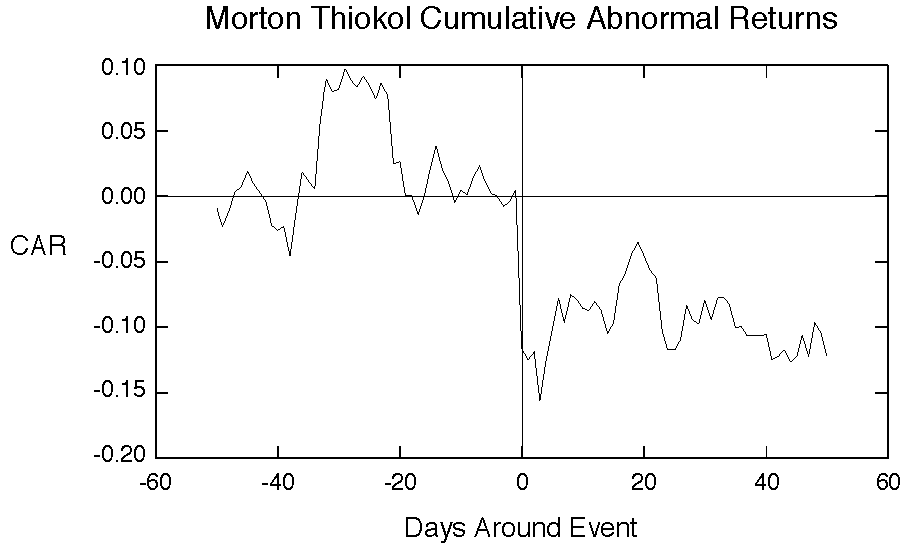
\includegraphics{thcar-final}
\end{center}
\caption{Morton Thiokol cumulative abnormal returns for 50
days before and after the event.}
\label{thcar}
\end{figure}
\clearpage



\section{Aftermath}

As a result of the space shuttle accident, Morton Thiokol was required to redesign the solid rocket boosters. {\em Business Week} of March 14, 1986 reported that, ``Thiokol has agreed to perform \$409 million worth of redesign work for NASA at no profit'' \cite[p. 91]{bw}. Another result of the accident is the Advanced Solid Rocket Booster (ASRB) project and Morton Thiokol failing to bid for the project. The ASRB project was a complete redesign of the solid rocket boosters ostensibly to provide more thrust (for bigger payloads and to take some of the work off the shuttle main engines). Morton Thiokol failed to bid for this project due to what some feared was political pressure. The contract for ASRBs called for the winner of the contract to design, develop, and test the motor with a delivery of six sets and an option for forty four more \cite[p. 13]{gao89}.

\section{Summary}

This chapter has shown that, as a result of the shuttle accident, firms involved in shuttle work should experience a decline in stock returns on the day of the accident. This was shown to be true, except for Morton Thiokol which experienced substantial negative returns. The suggested cause of this negative return was the aftermath of the accident Morton Thiokol, the at-fault company. The return would be expected to be especially large because the problem that resulted in the accident---the failure of the shuttle's O-rings---was known by engineers in NASA and Morton Thiokol. In fact, Morton Thiokol did face losses in addition to the loss of sales during the time the shuttle program was shutdown. That is, they dropped out of bidding for the next generation of solid rocket boosters, although they (in 1984) manufactured some fifty percent of all the boosters manufactured in the United States \cite[p. 18]{gao86}. They also performed redesign work on the solid rocket boosters at no profit.

